\documentclass[12pt, a4paper]{book}
\begin{document}

\chapter{Data and MC agreement of jets in preselection region}\label{appendix:JetSelection}
\graphicspath{{../../Plots/Data_Analysis/JetSelection/Control_region/}} 
\begin{figure}[!ht]
    \centering
    \begin{subfigure}[b]{0.49\textwidth}
        \centering
        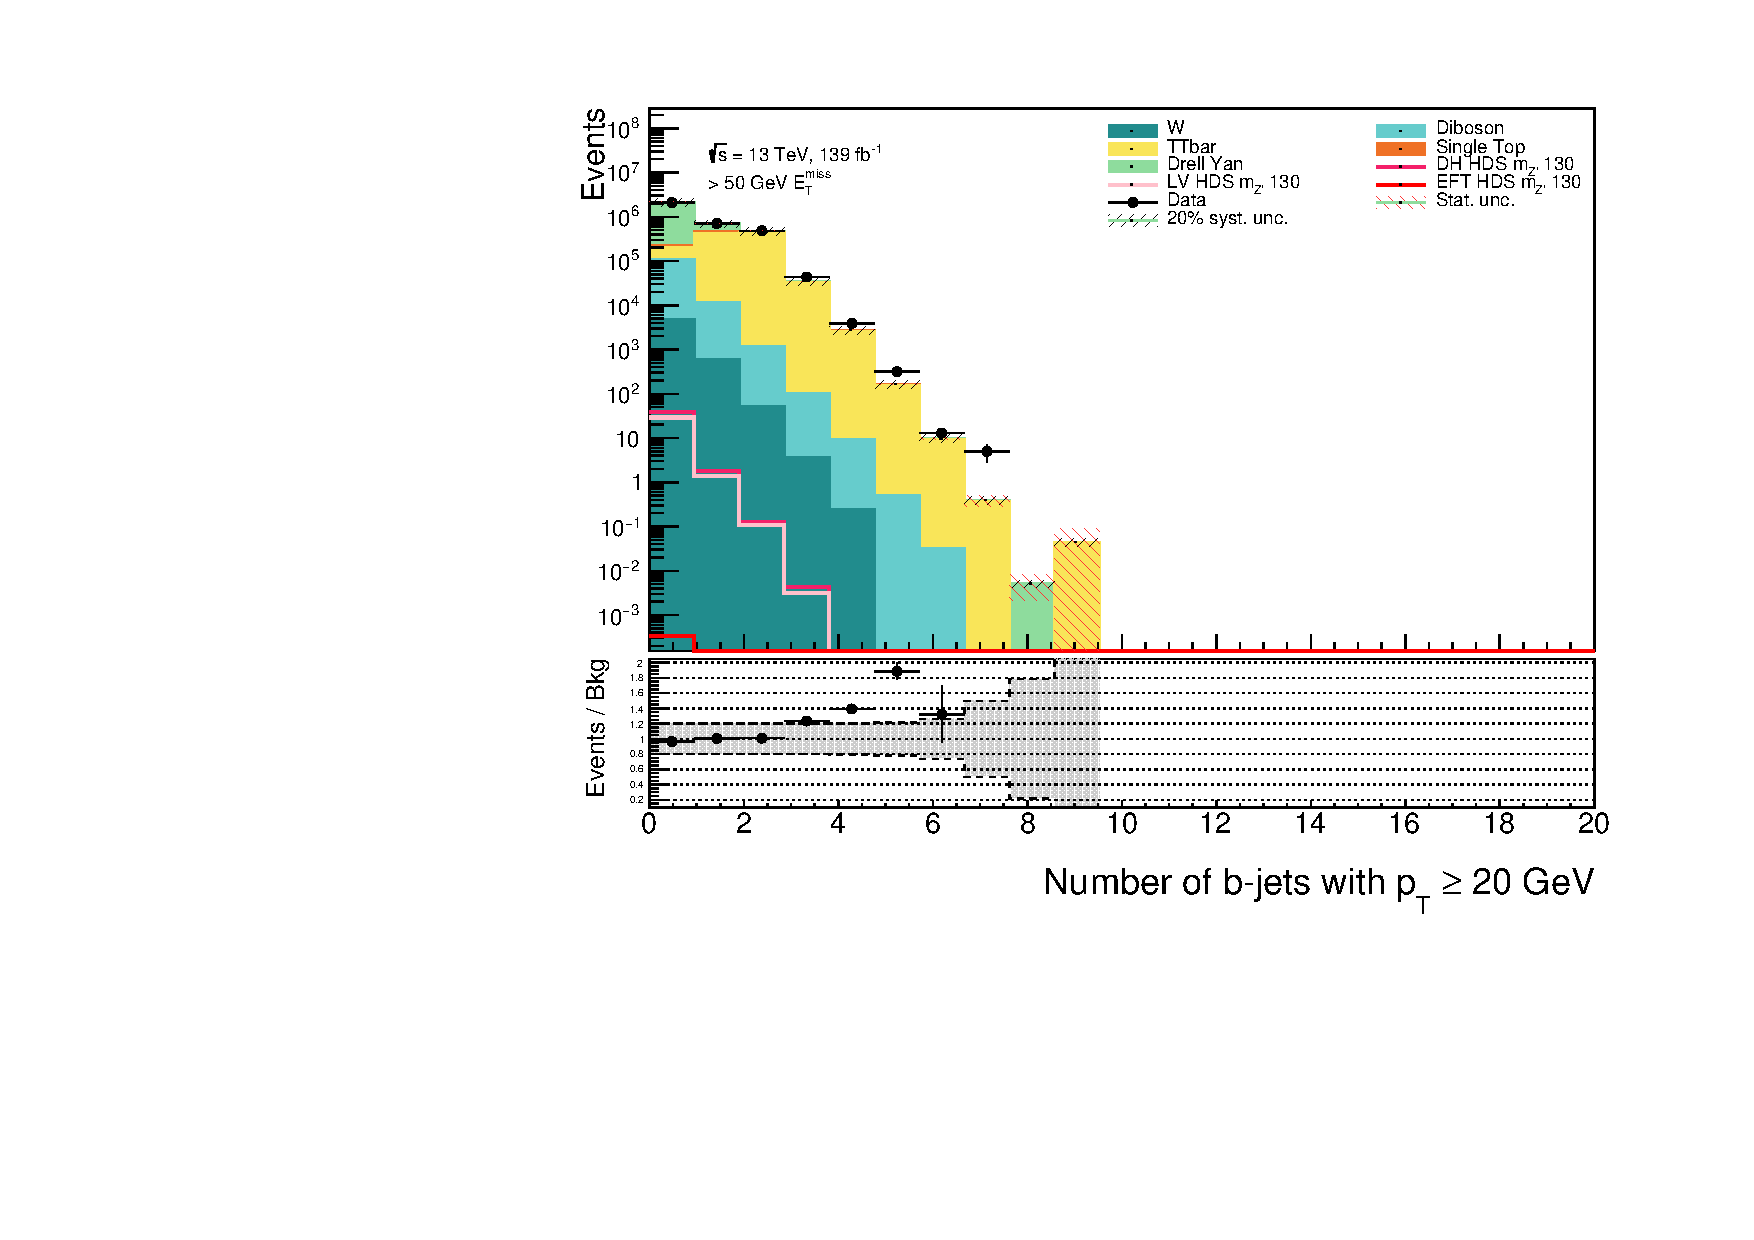
\includegraphics[width=\textwidth]{bjetsPt20.pdf}
    \end{subfigure}
    \hfill\begin{subfigure}[b]{0.49\textwidth}
        \centering
        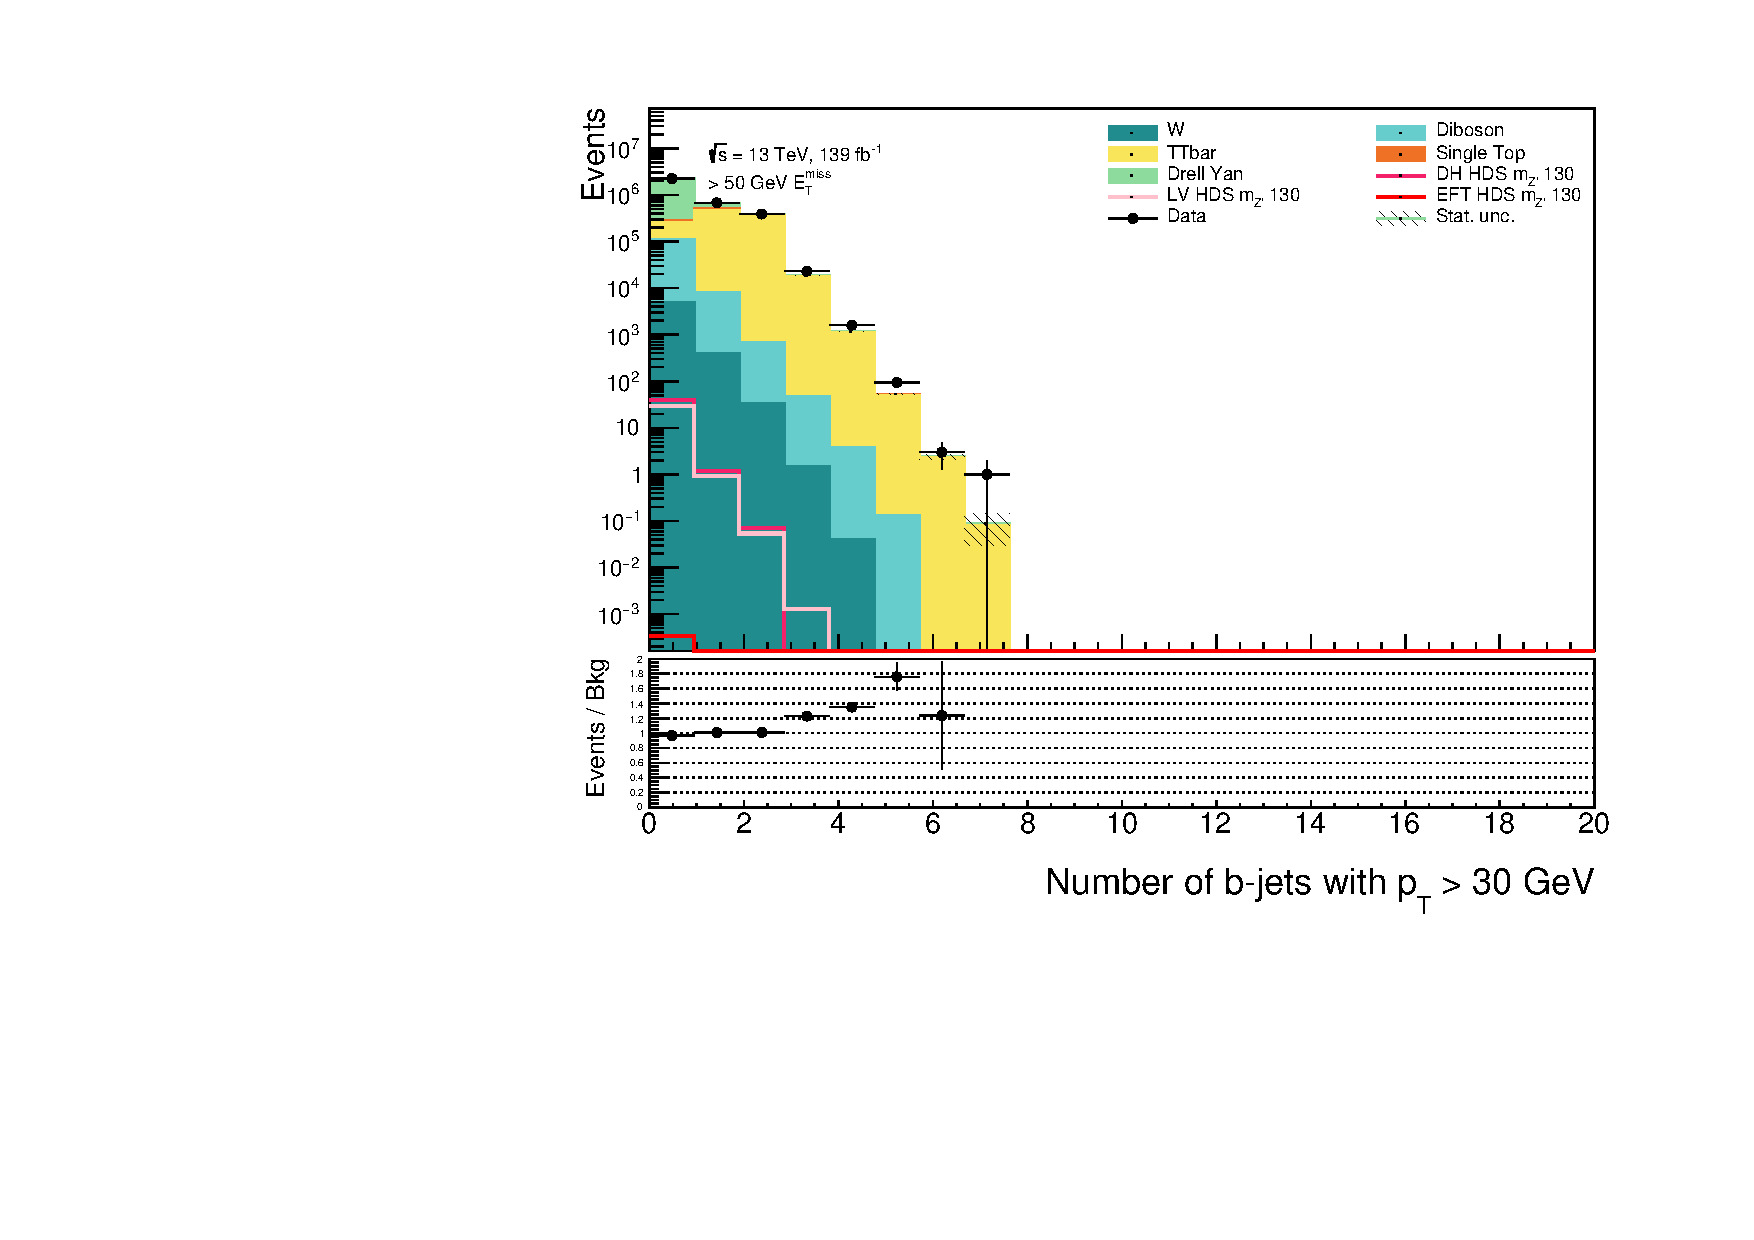
\includegraphics[width=\textwidth]{bjetsPt30.pdf}
    \end{subfigure}
    \hfill\begin{subfigure}[b]{0.49\textwidth}
        \centering
        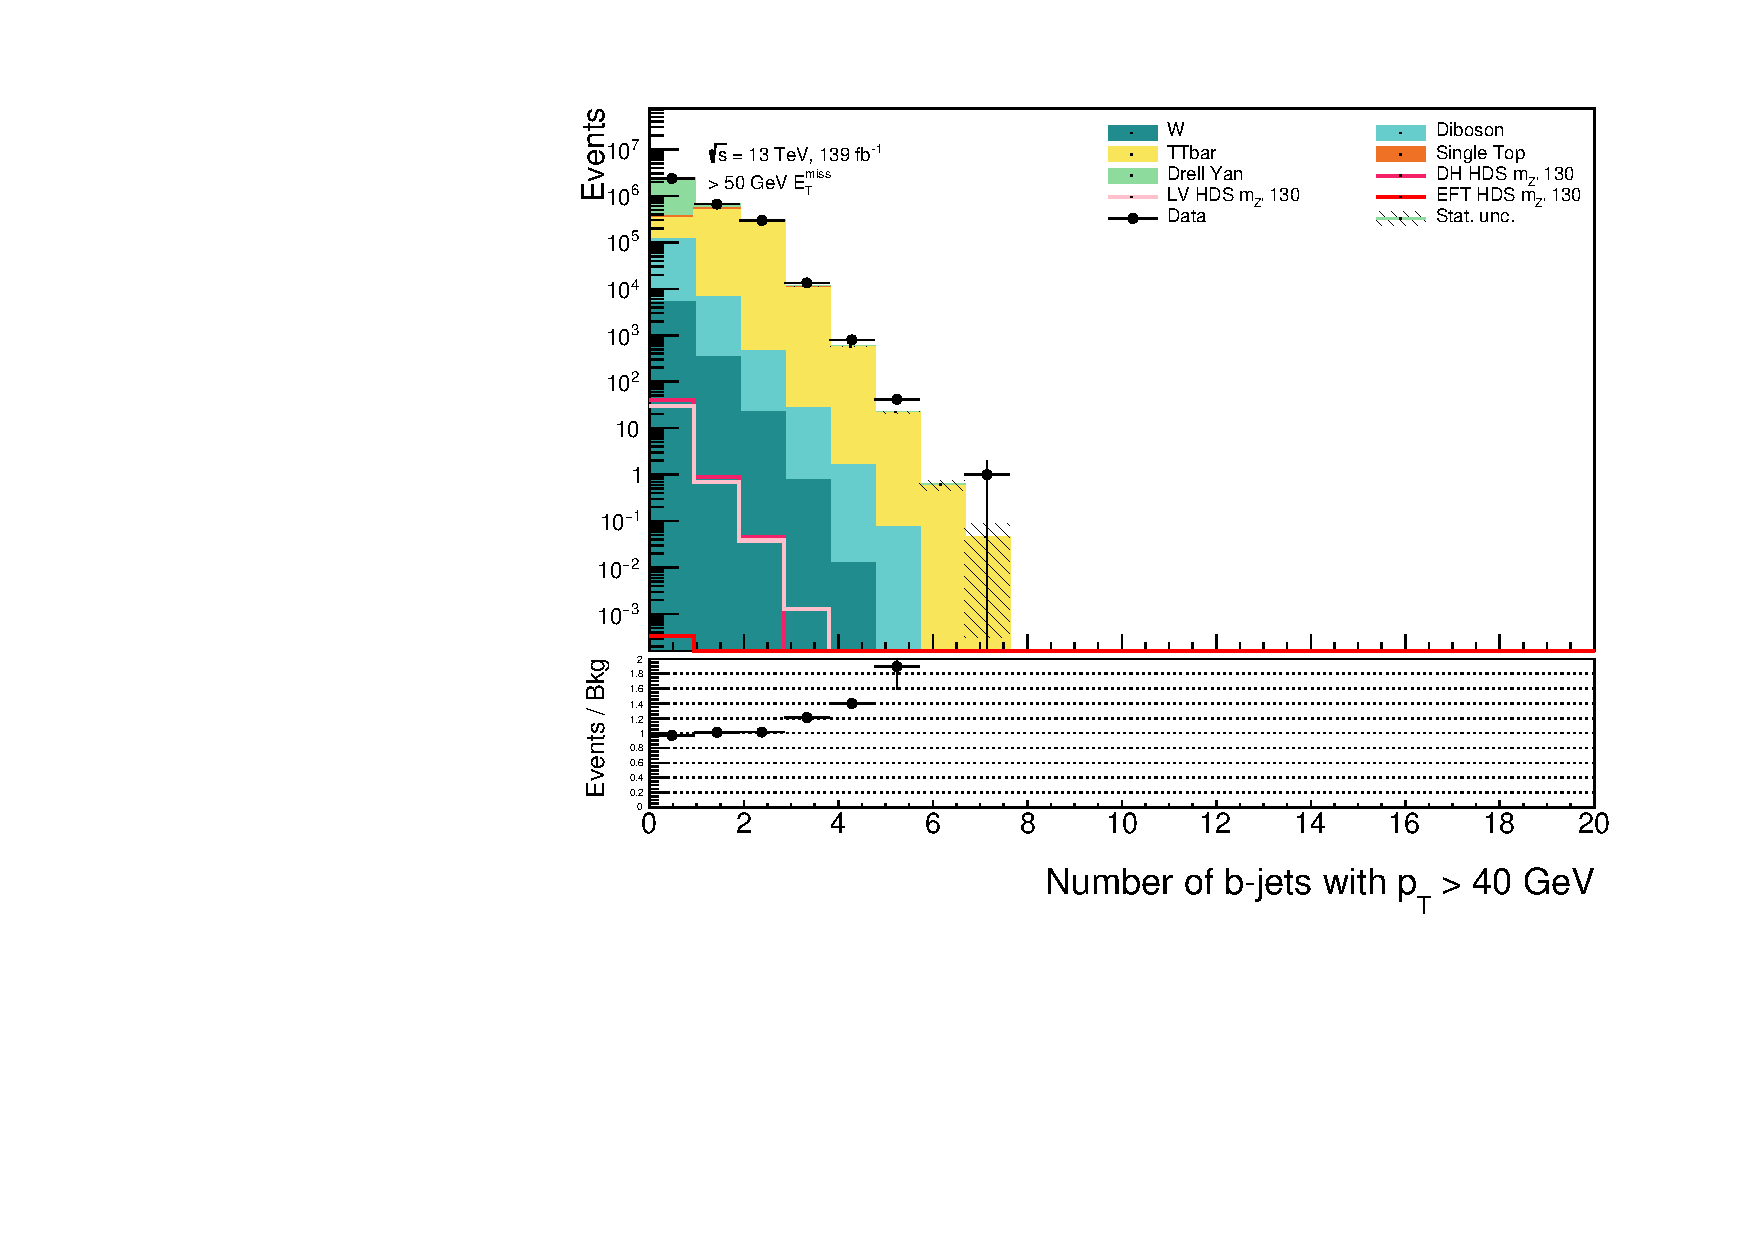
\includegraphics[width=\textwidth]{bjetsPt40.pdf}
    \end{subfigure}
    \hfill\begin{subfigure}[b]{0.49\textwidth}
        \centering
        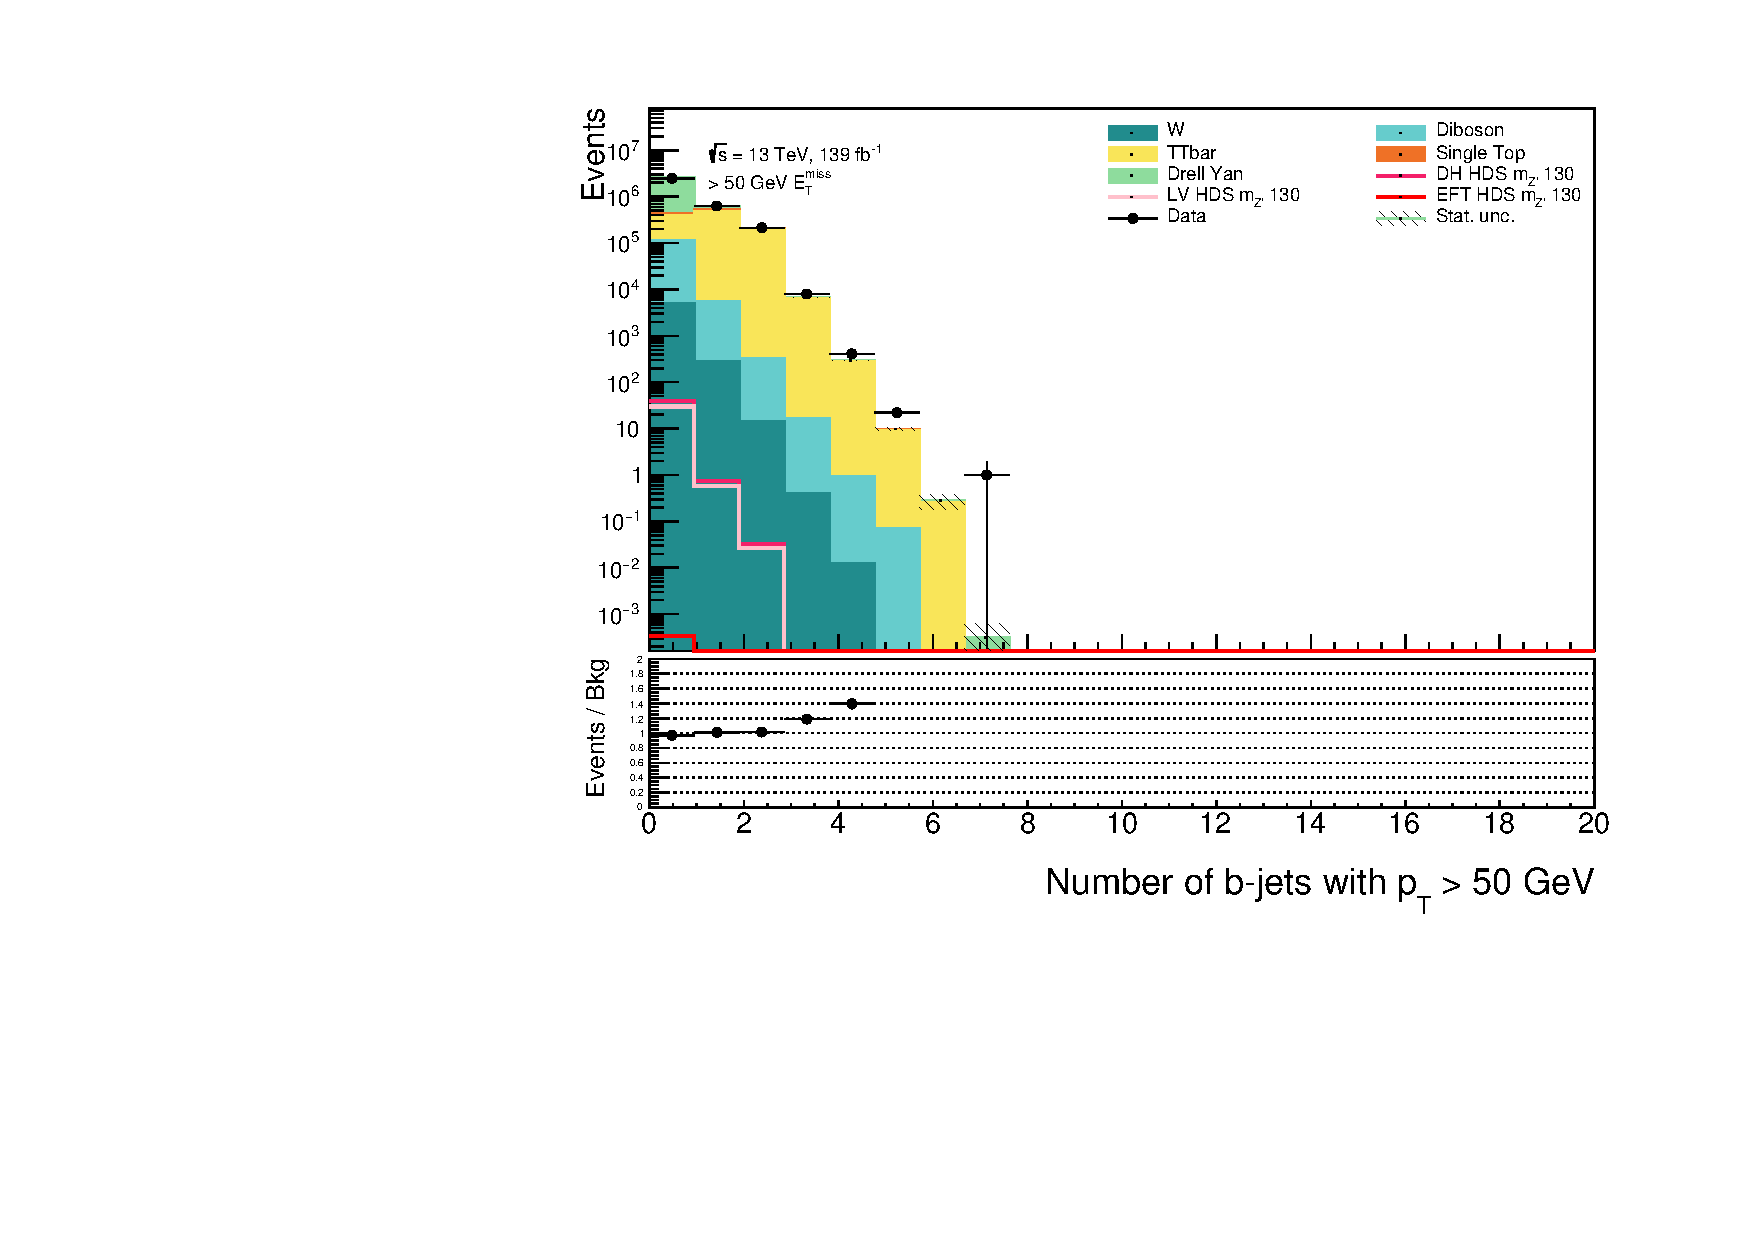
\includegraphics[width=\textwidth]{bjetsPt50.pdf}
    \end{subfigure}
    \hfill\begin{subfigure}[b]{0.49\textwidth}
        \centering
        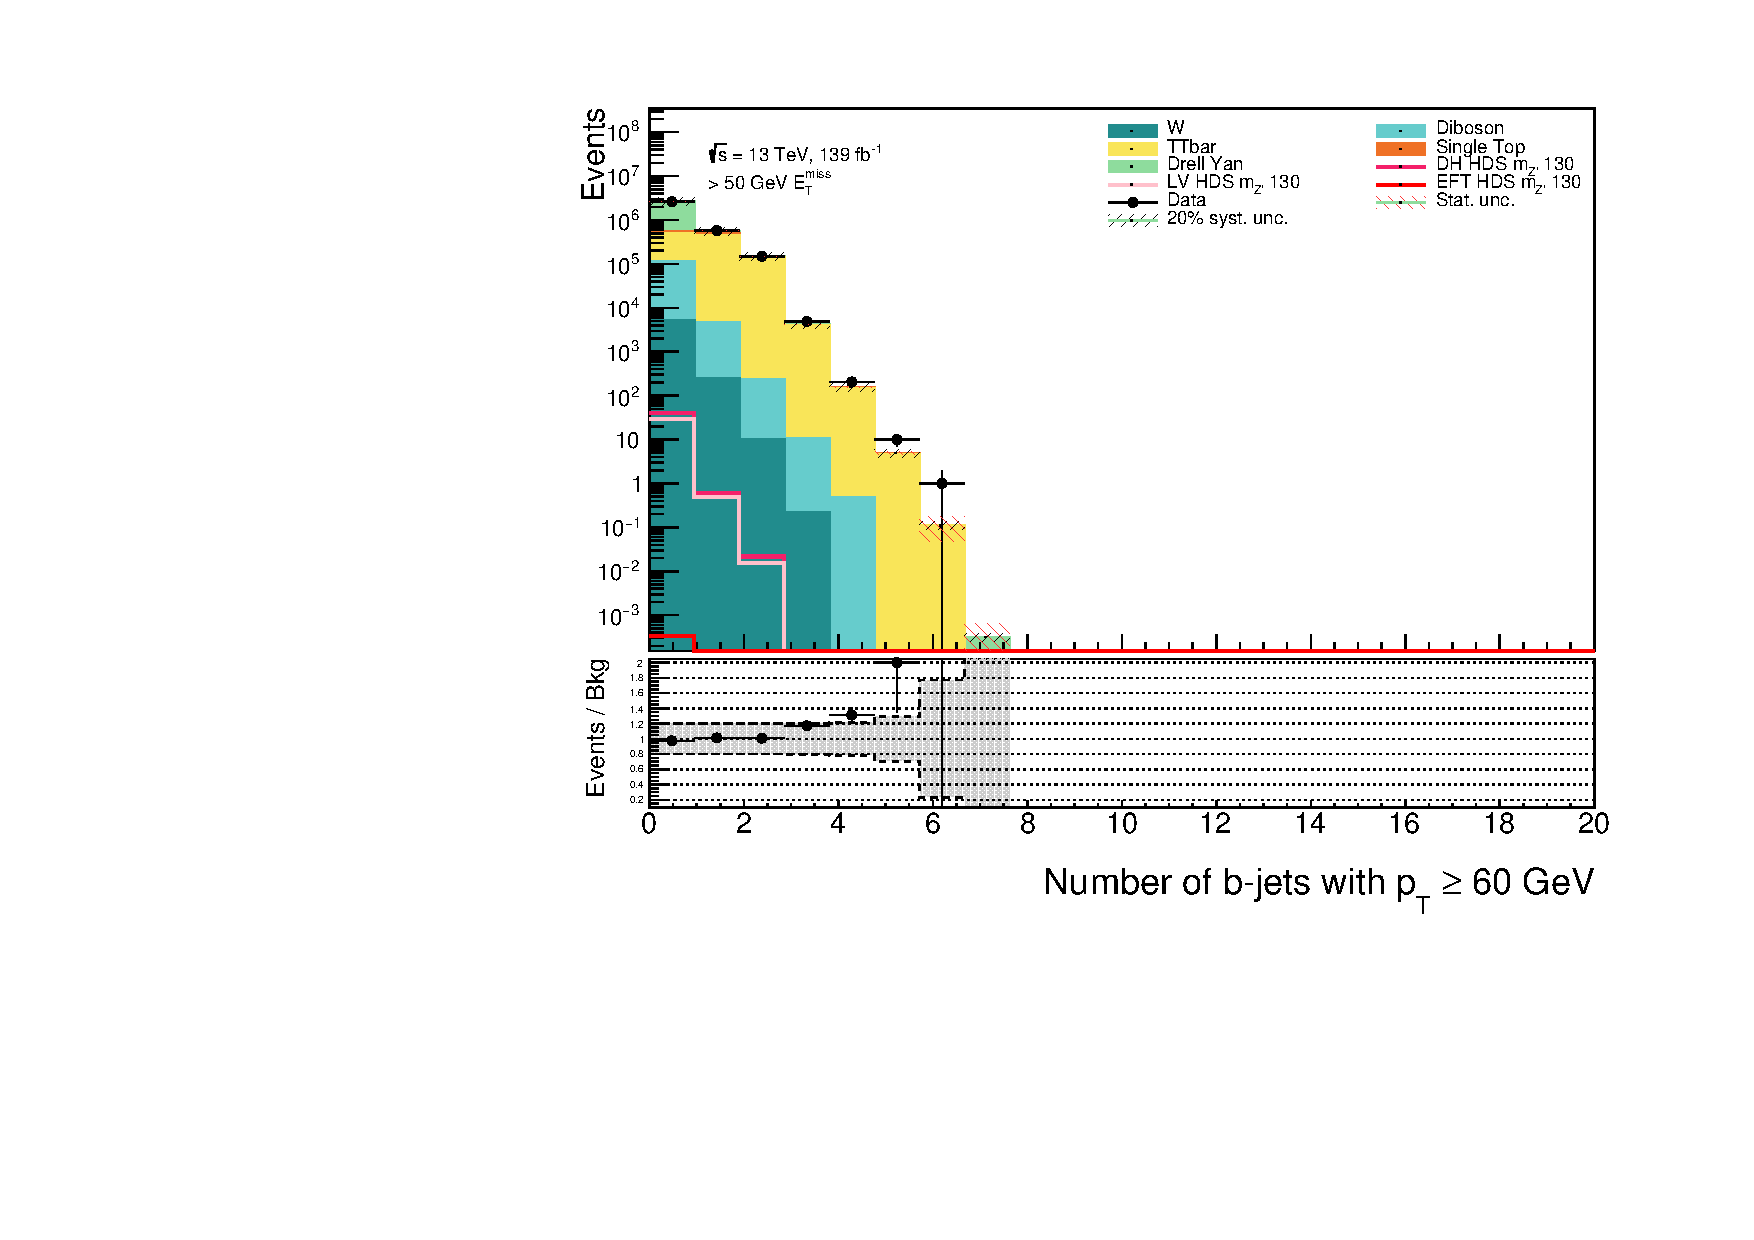
\includegraphics[width=\textwidth]{bjetsPt60.pdf}
    \end{subfigure}
    \caption{Data and MC agreement on number of b- jets with different $p_T$ cuts in CR.}
\end{figure}

\begin{figure}[!ht]
    \centering
    \begin{subfigure}[b]{0.49\textwidth}
        \centering
        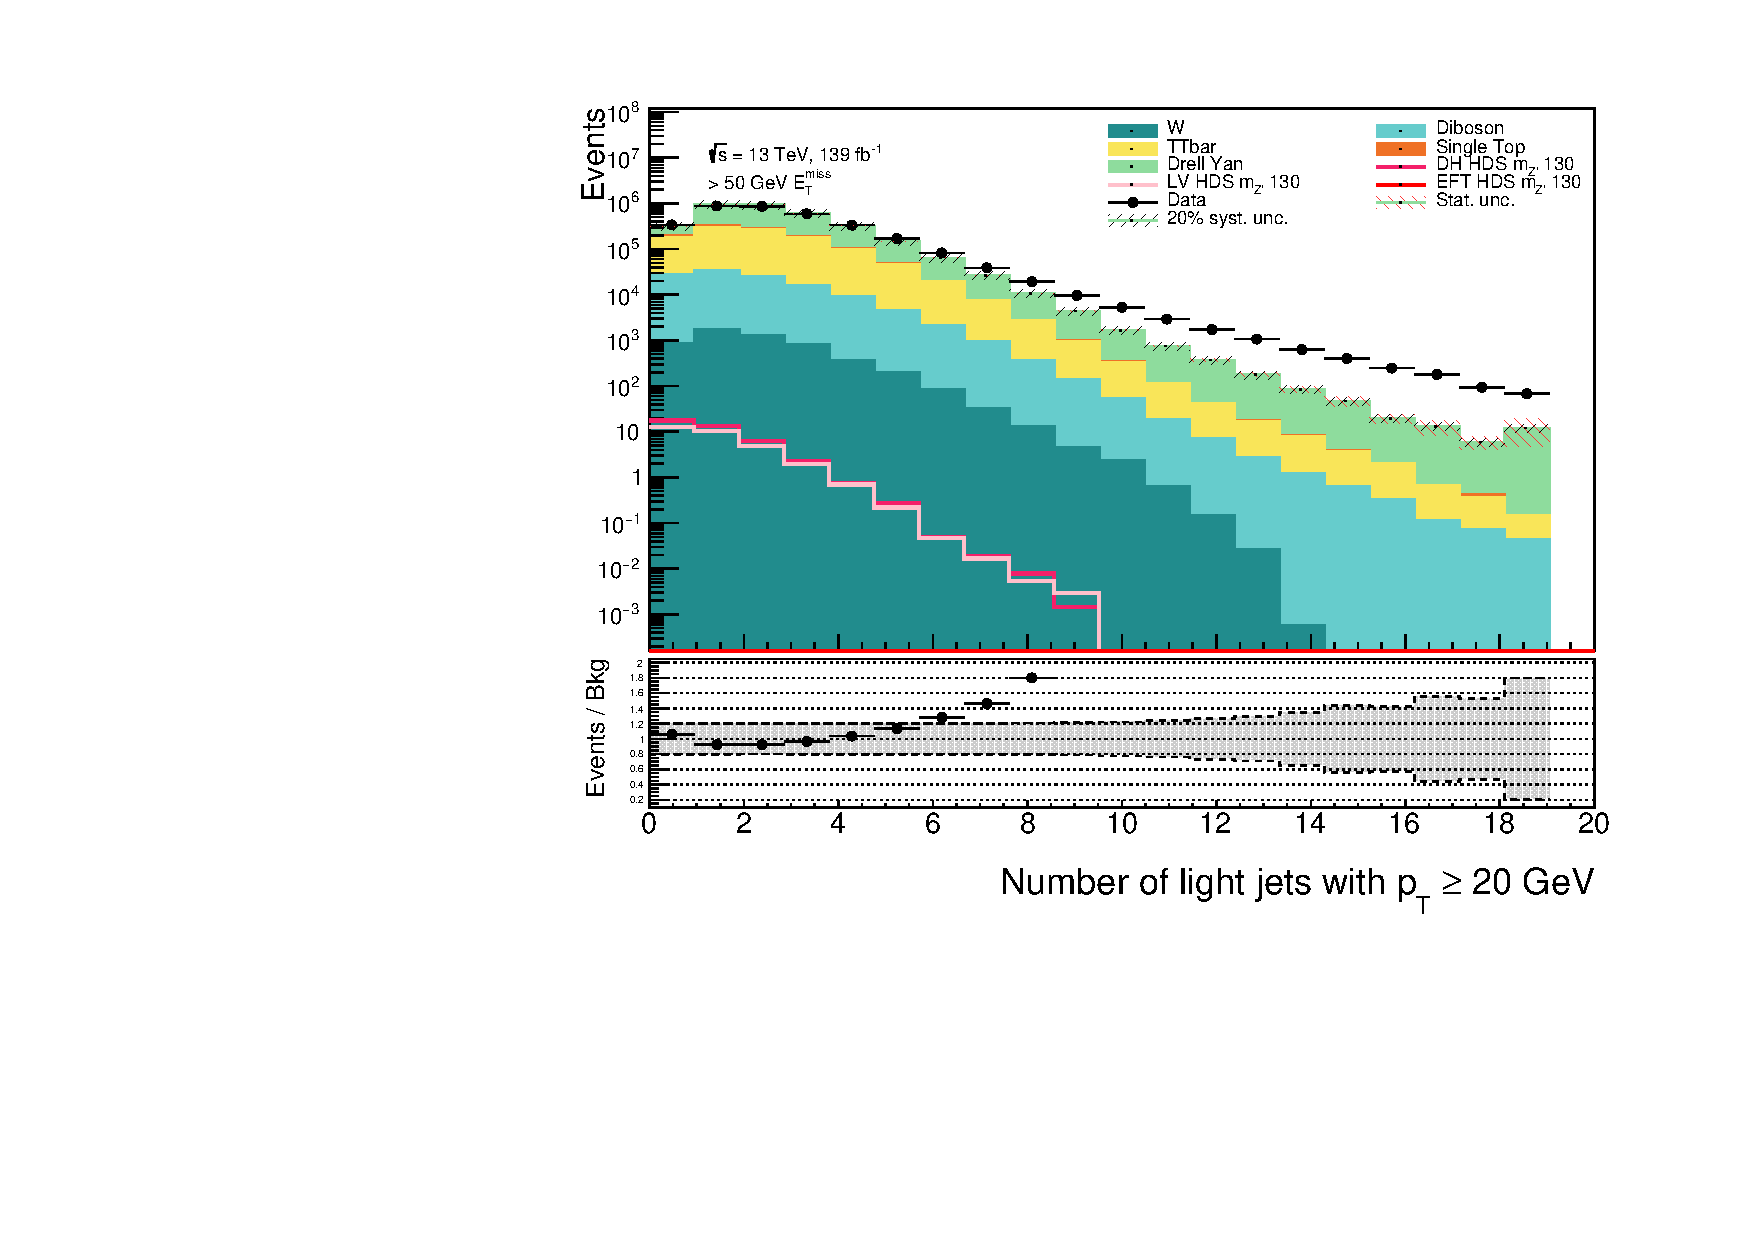
\includegraphics[width=\textwidth]{ljetsPt20.pdf}
    \end{subfigure}
    \hfill\begin{subfigure}[b]{0.49\textwidth}
        \centering
        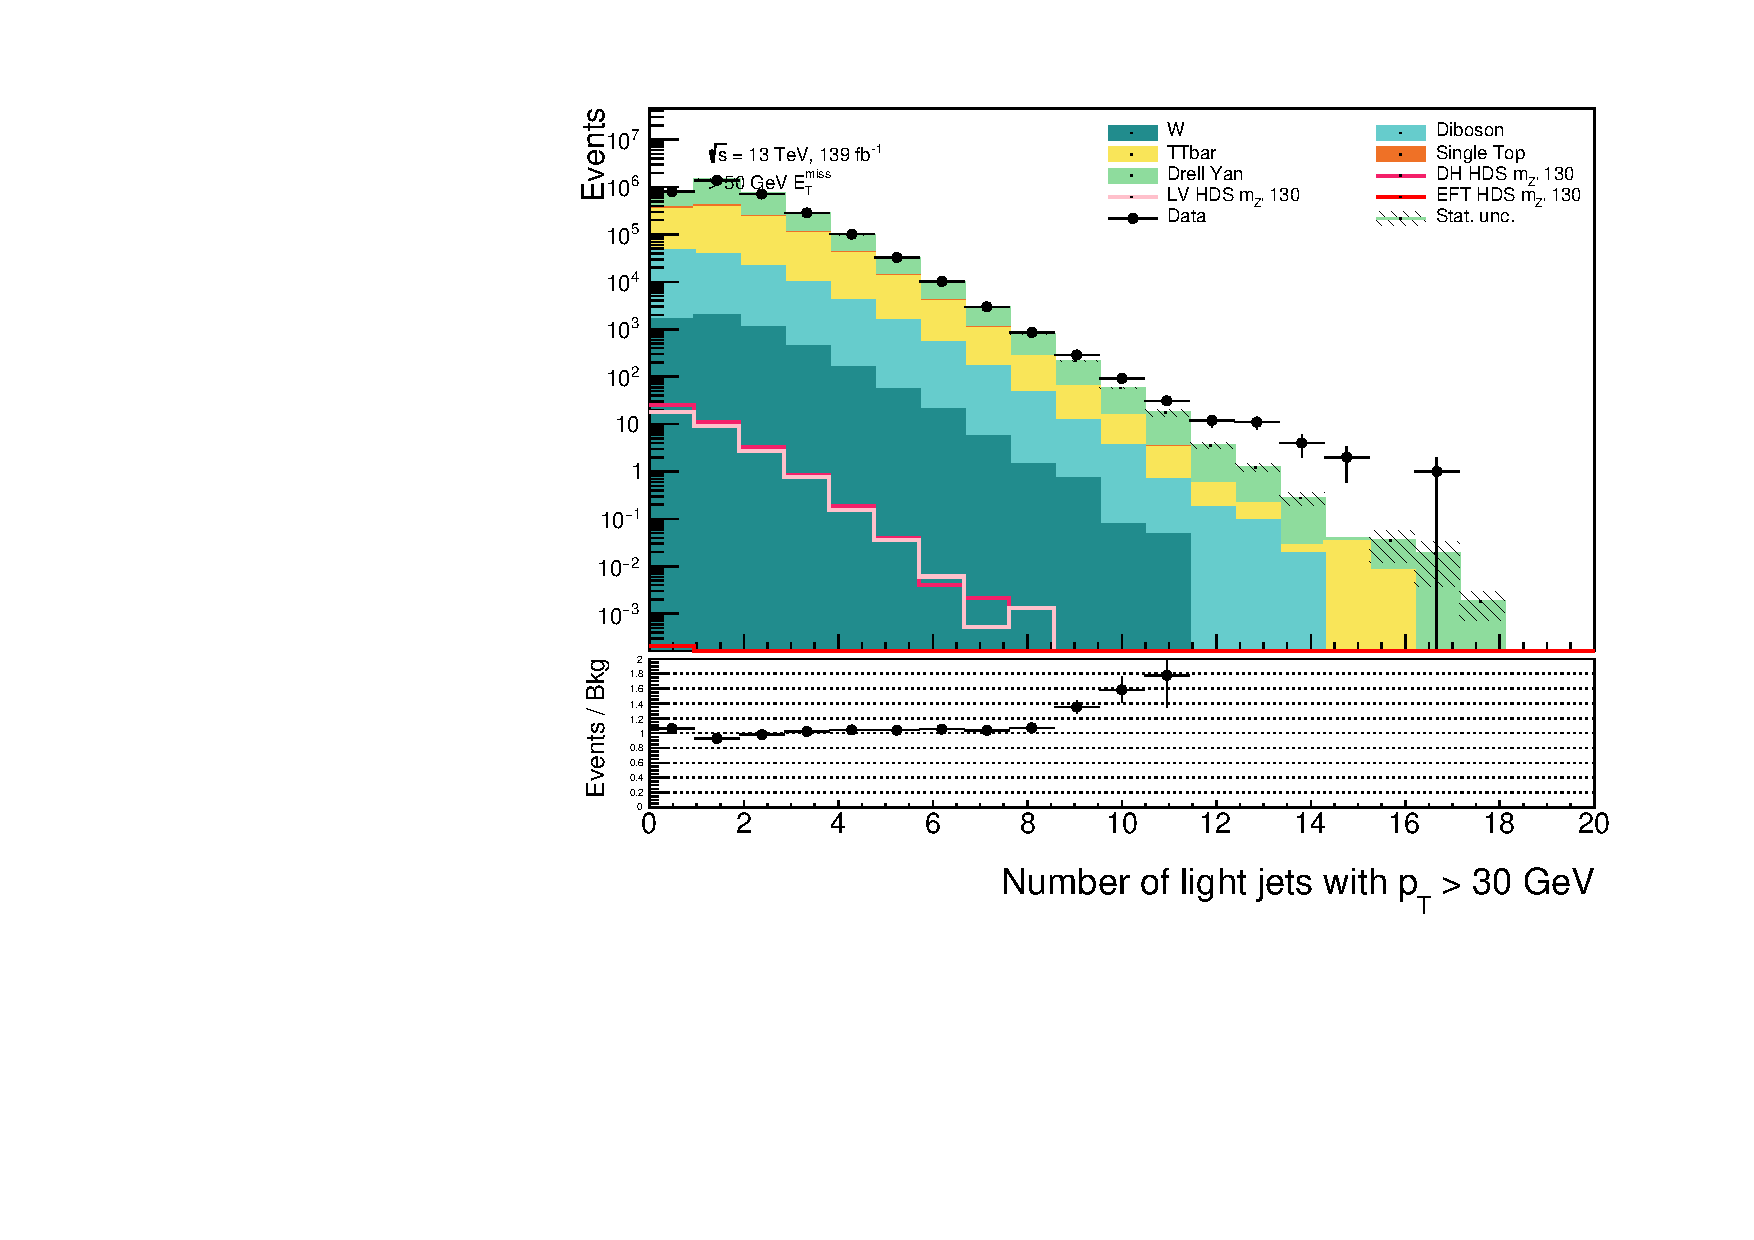
\includegraphics[width=\textwidth]{ljetsPt30.pdf}
    \end{subfigure}
    \hfill\begin{subfigure}[b]{0.49\textwidth}
        \centering
        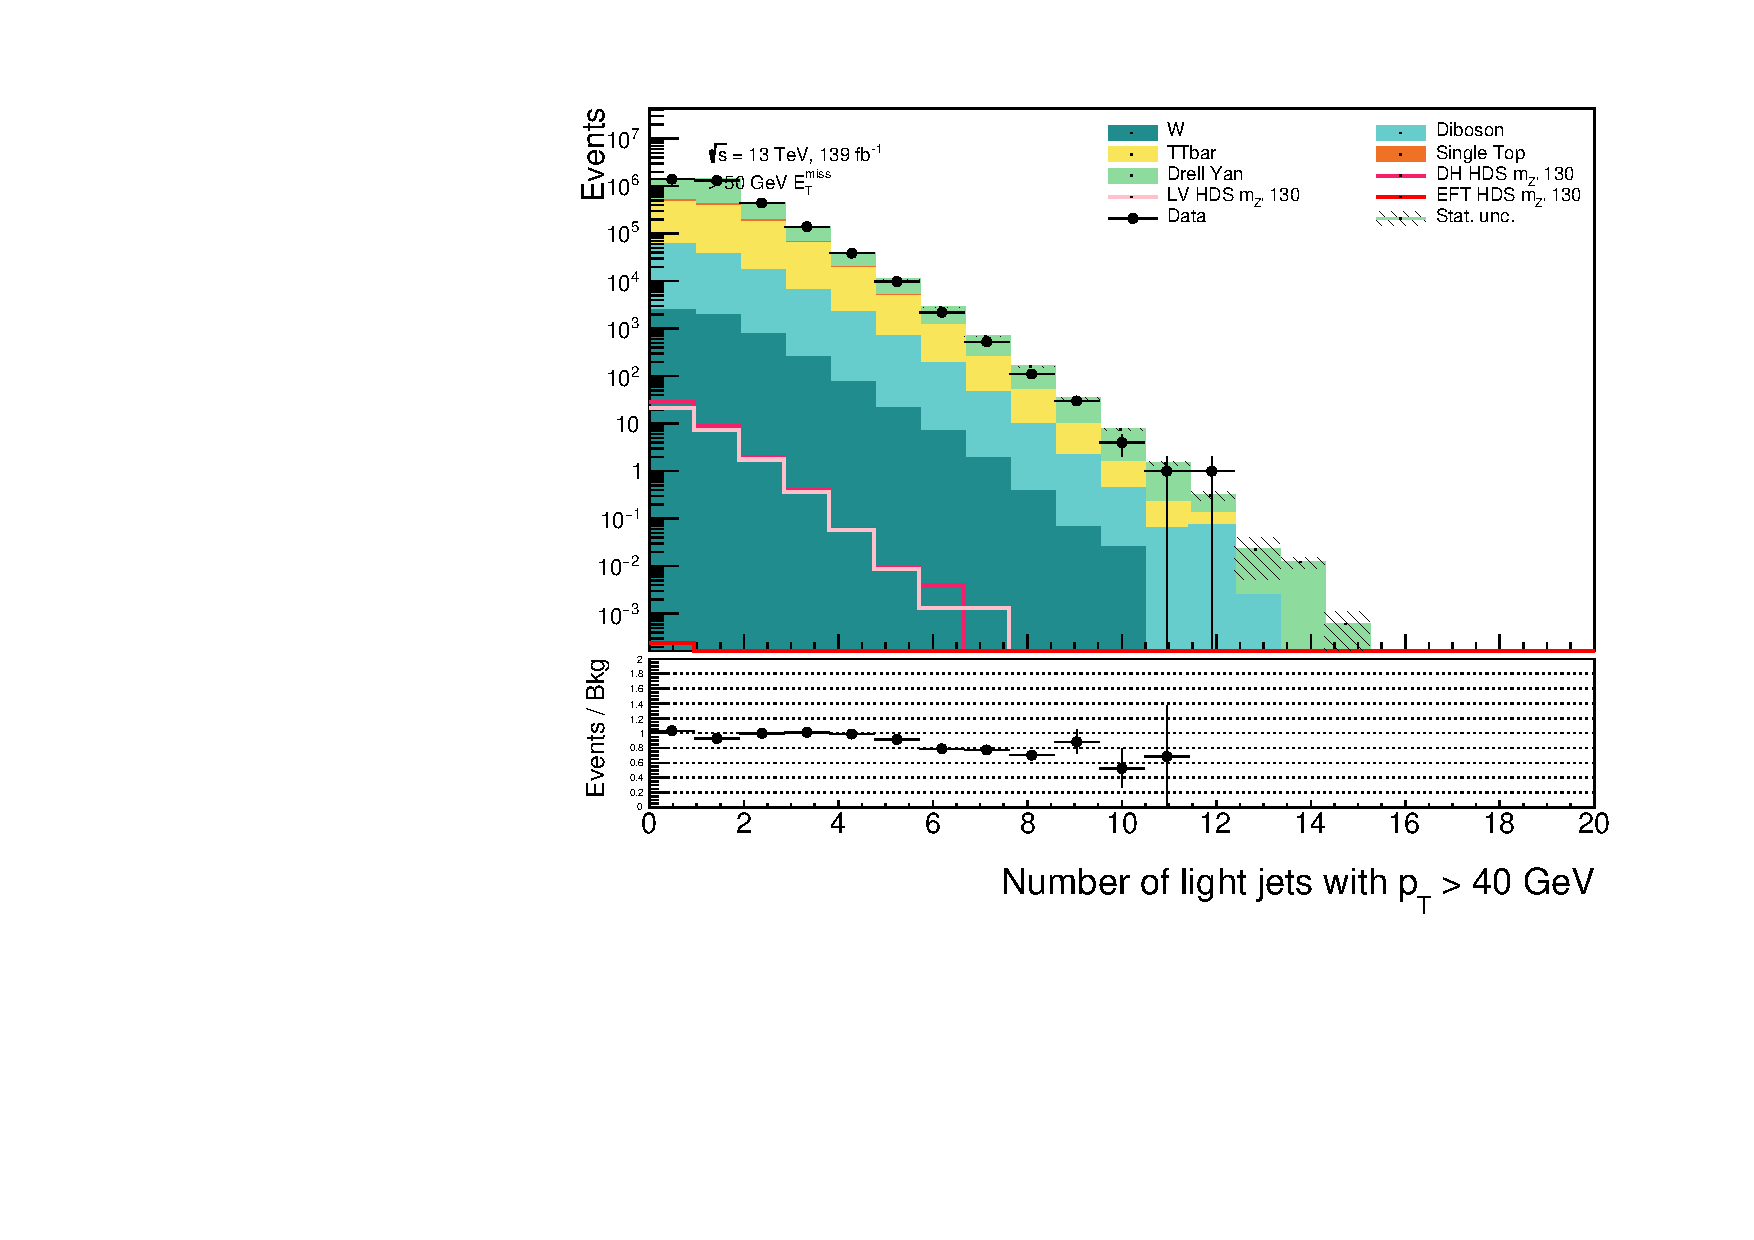
\includegraphics[width=\textwidth]{ljetsPt40.pdf}
    \end{subfigure}
    \hfill\begin{subfigure}[b]{0.49\textwidth}
        \centering
        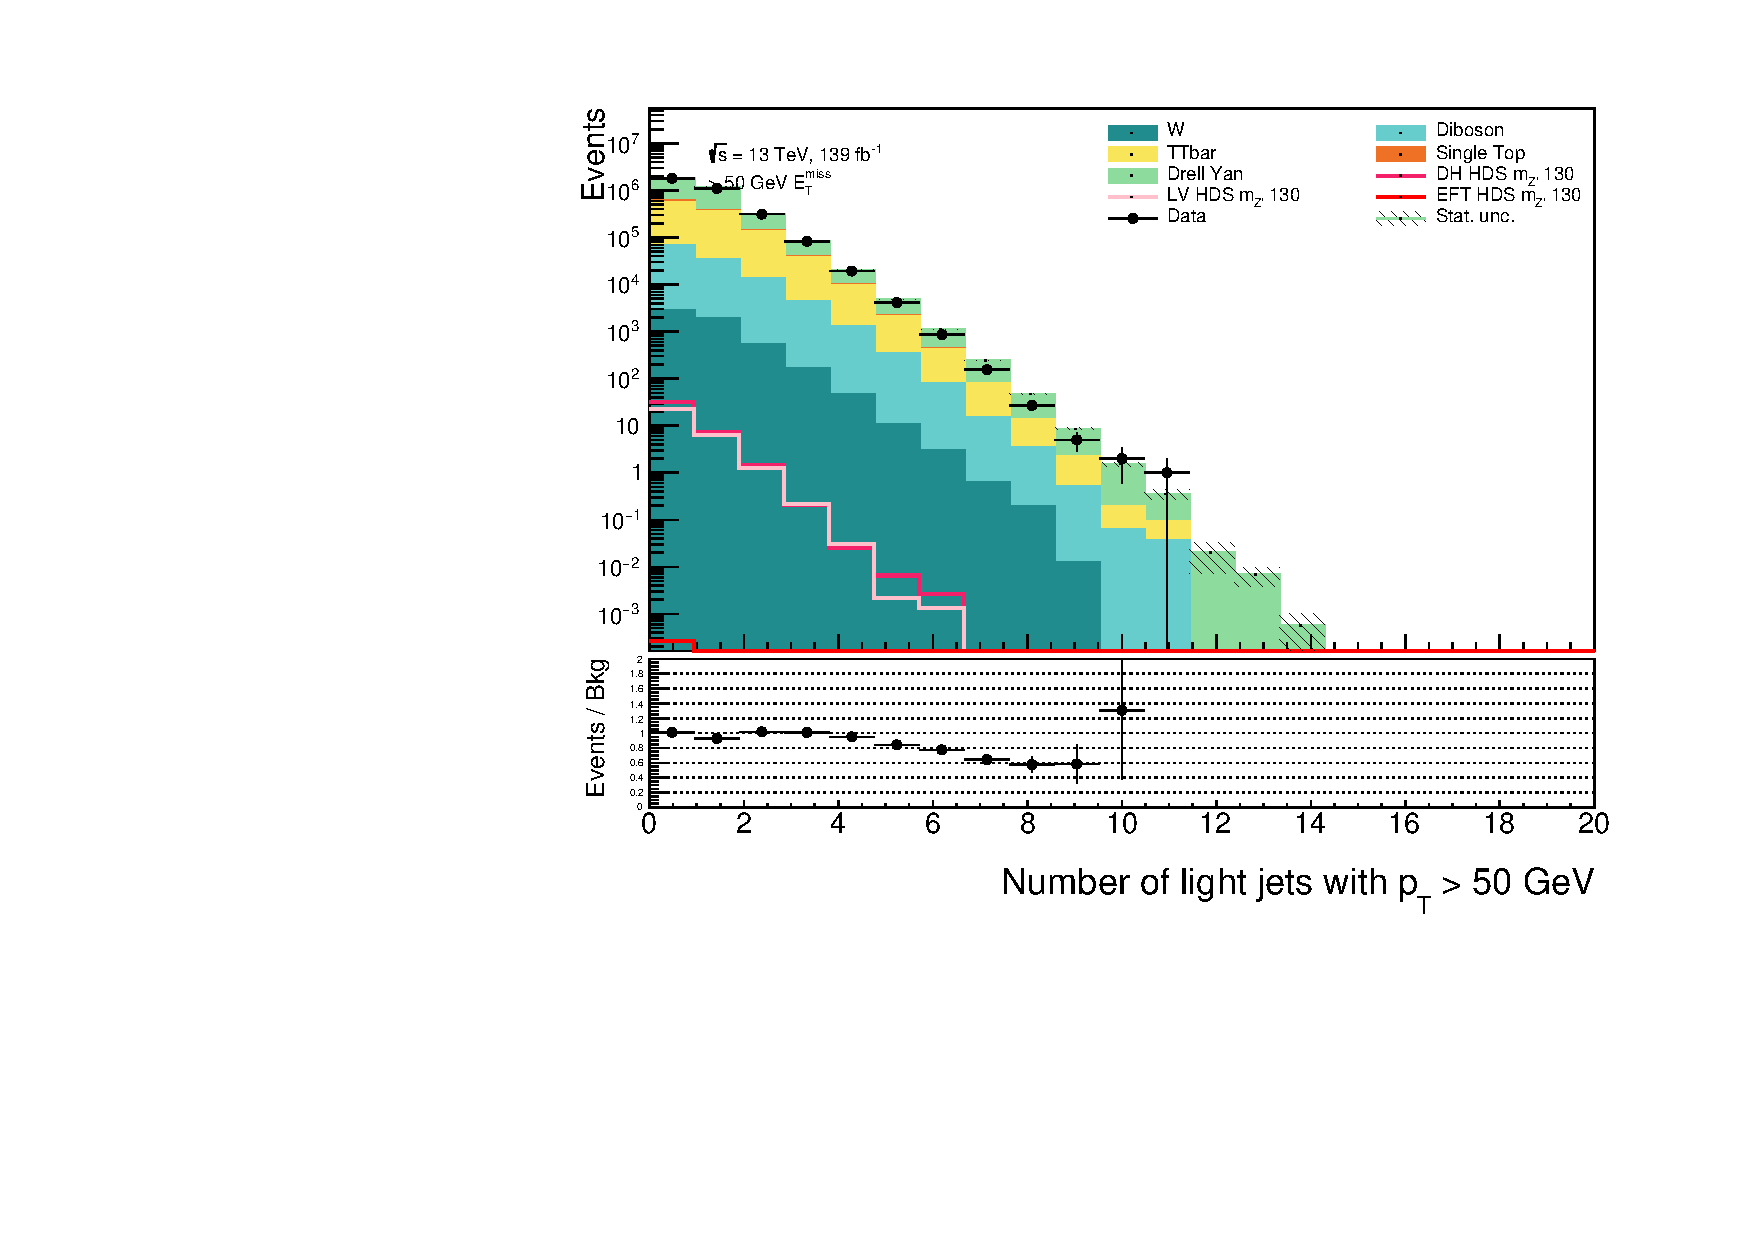
\includegraphics[width=\textwidth]{ljetsPt50.pdf}
    \end{subfigure}
    \hfill\begin{subfigure}[b]{0.49\textwidth}
        \centering
        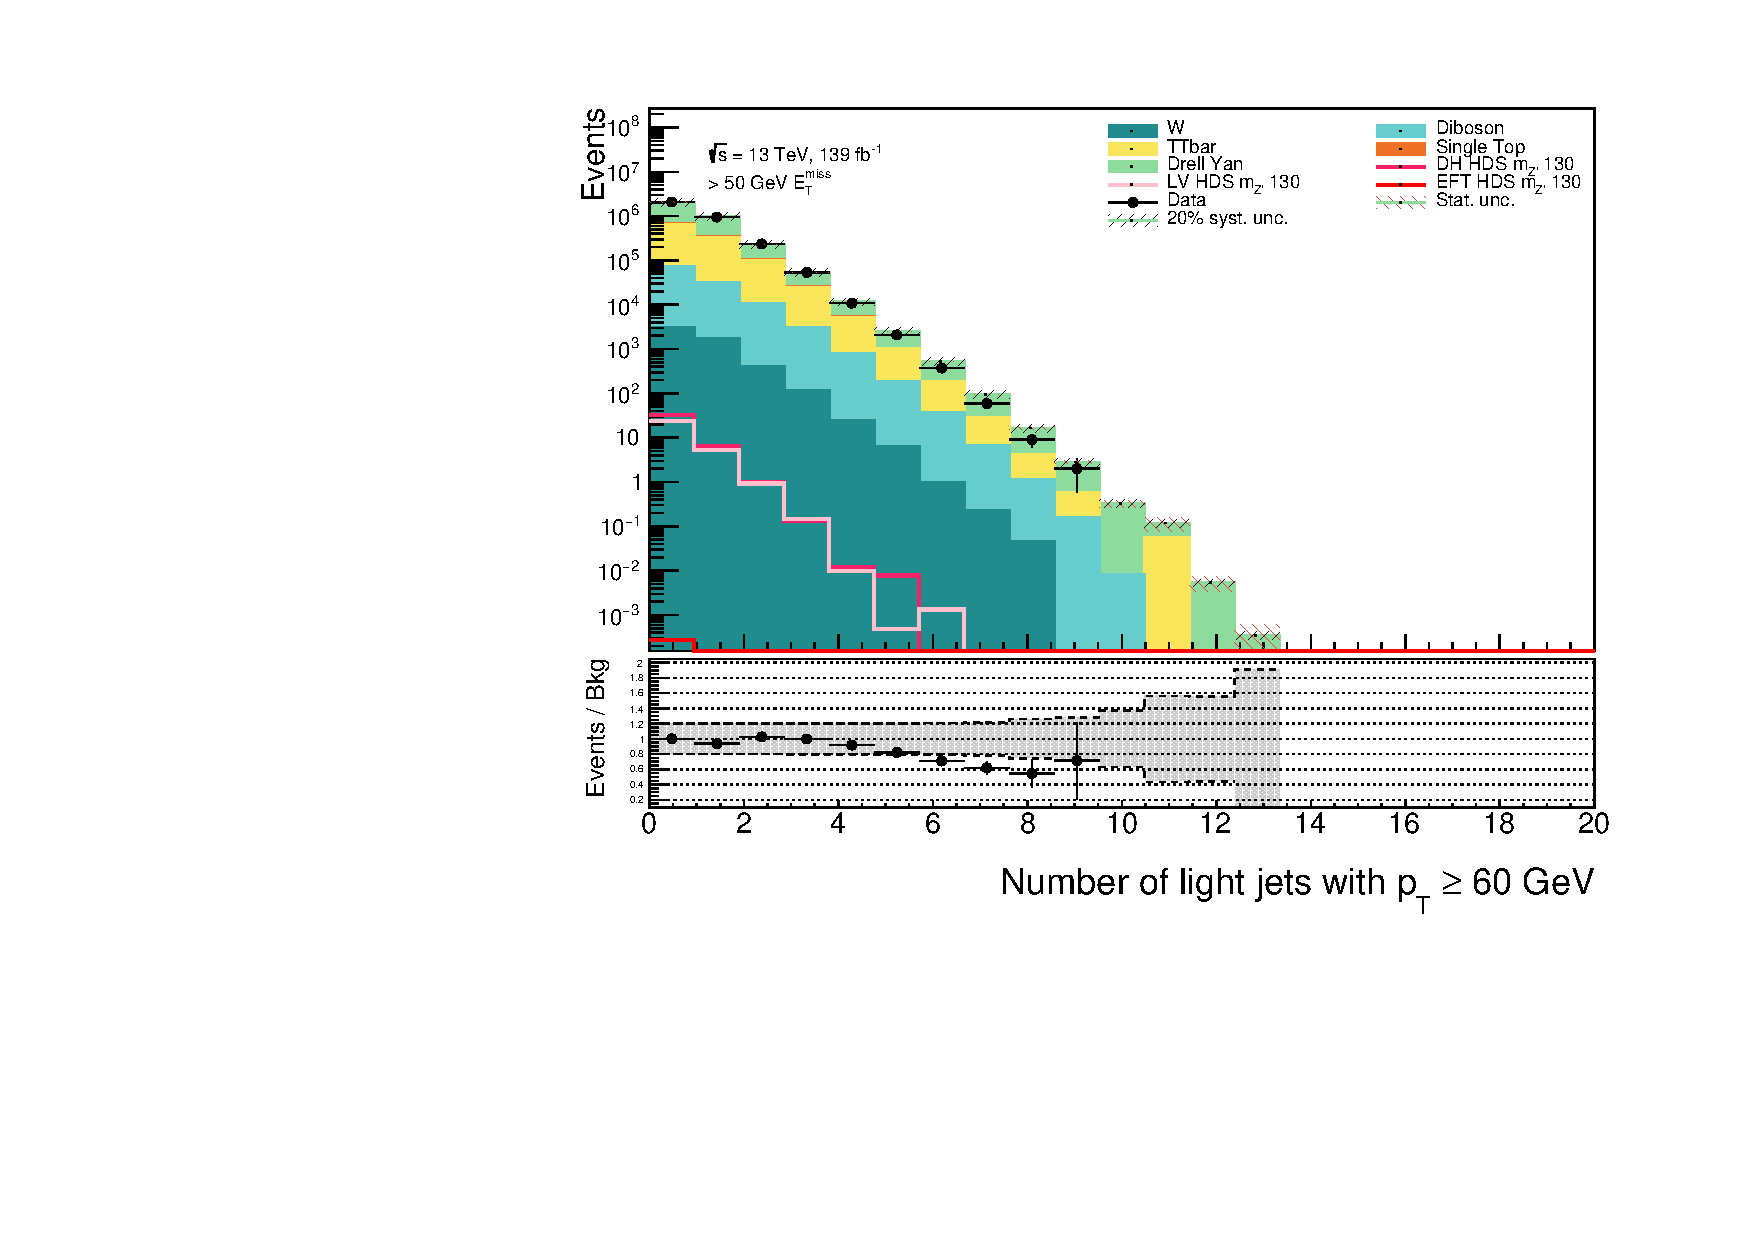
\includegraphics[width=\textwidth]{ljetsPt60.pdf}
    \end{subfigure}
    \caption{Data and MC agreement on number of light jets with different $p_T$ cuts in CR.}
\end{figure}

% \graphicspath{{../../Plots/Data_Analysis/JetSelection/Uncut/}} 
% \begin{figure}[!ht]
%     \centering
%     \begin{subfigure}[b]{0.49\textwidth}
%         \centering
%         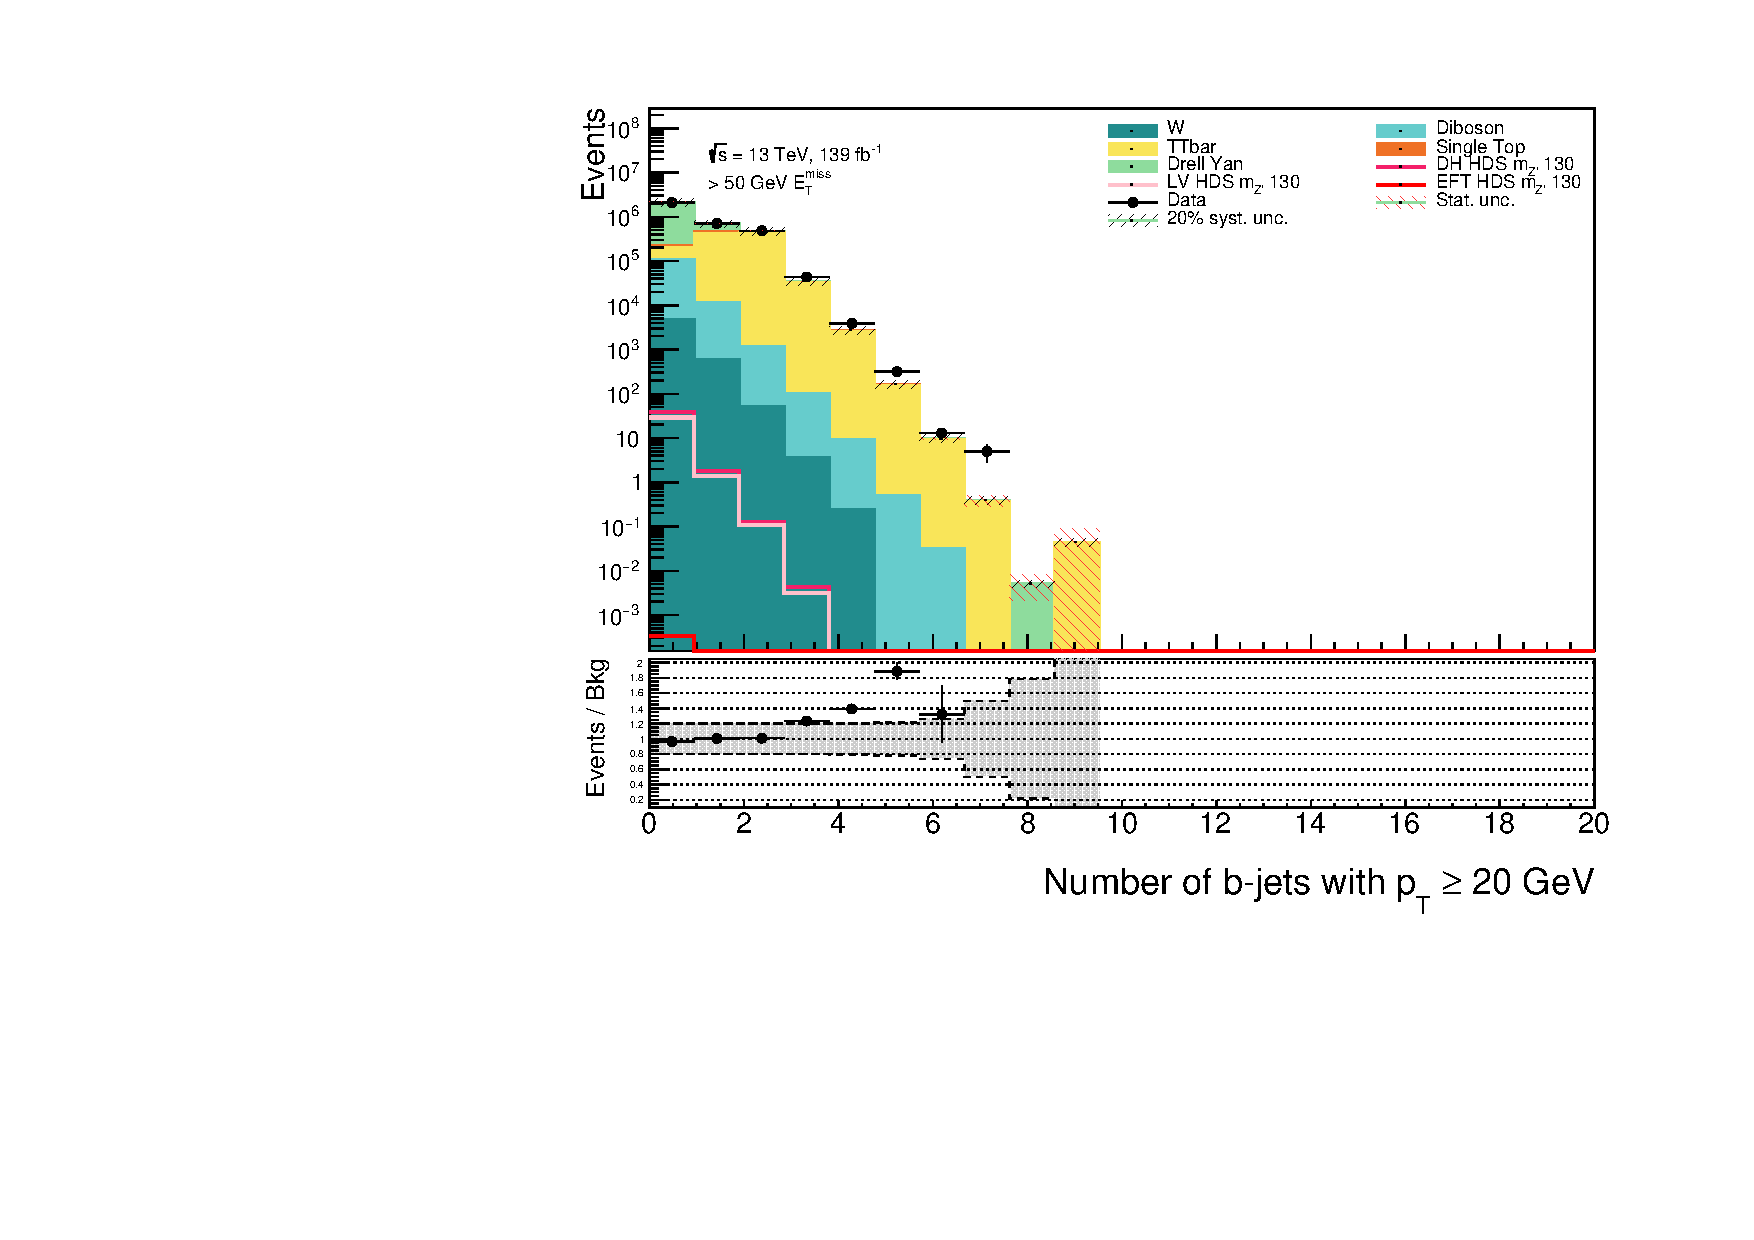
\includegraphics[width=\textwidth]{bjetsPt20.pdf}
%     \end{subfigure}
%     \hfill\begin{subfigure}[b]{0.49\textwidth}
%         \centering
%         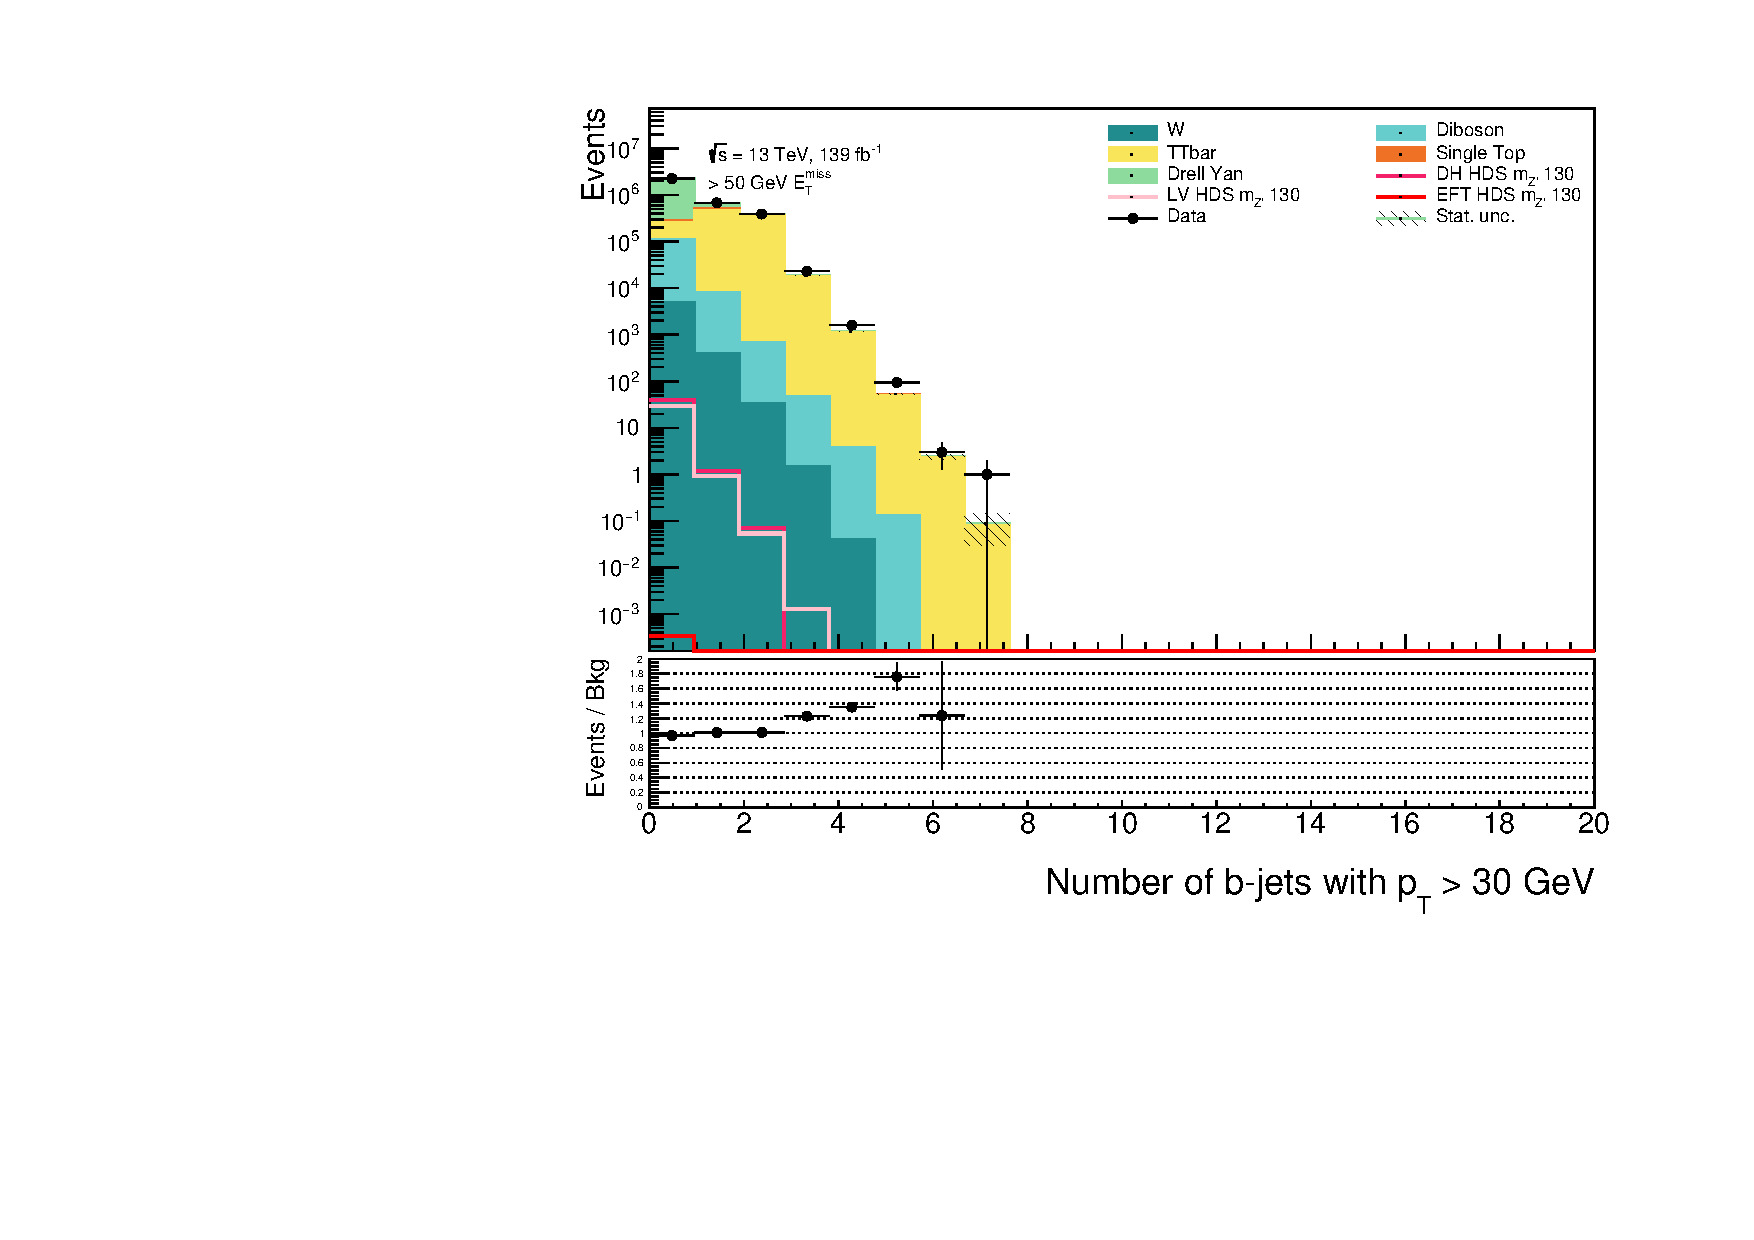
\includegraphics[width=\textwidth]{bjetsPt30.pdf}
%     \end{subfigure}
%     \hfill\begin{subfigure}[b]{0.49\textwidth}
%         \centering
%         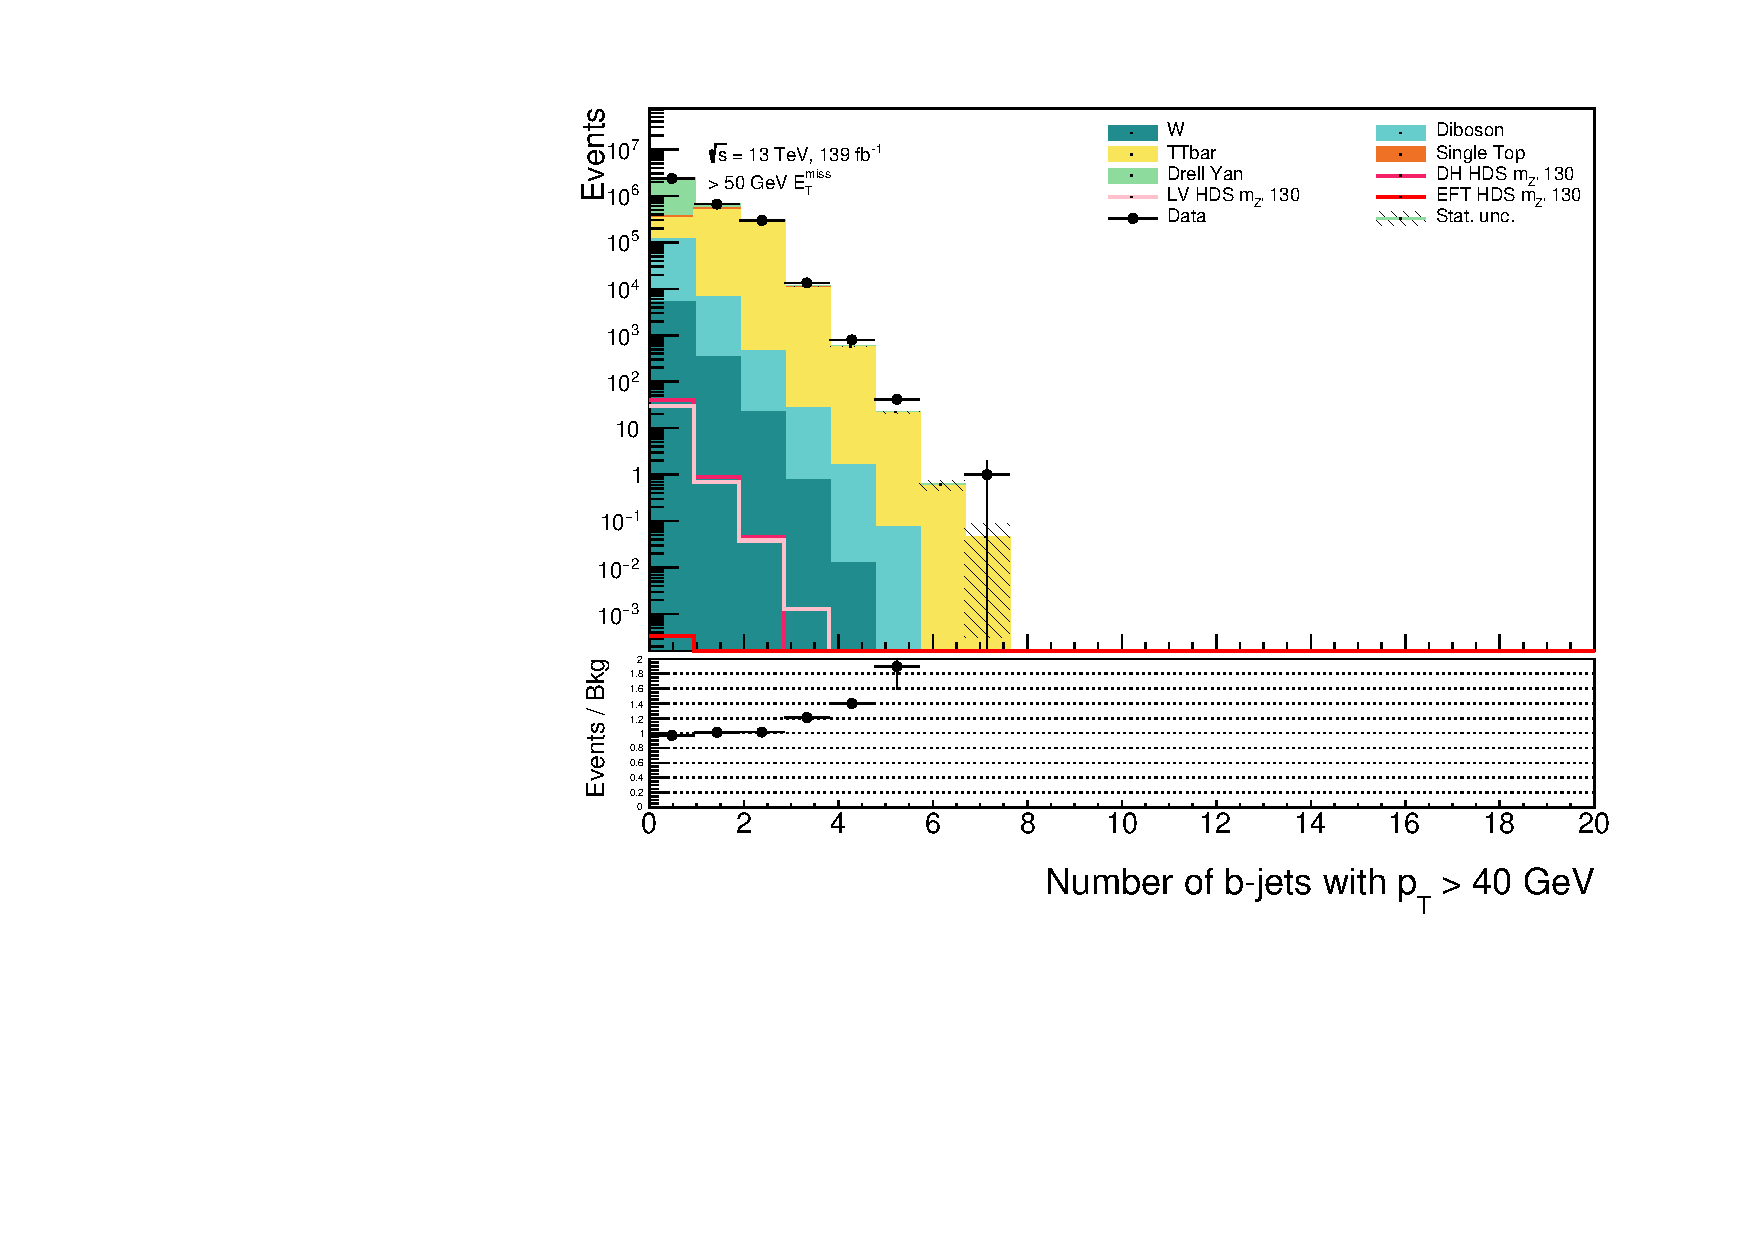
\includegraphics[width=\textwidth]{bjetsPt40.pdf}
%     \end{subfigure}
%     \hfill\begin{subfigure}[b]{0.49\textwidth}
%         \centering
%         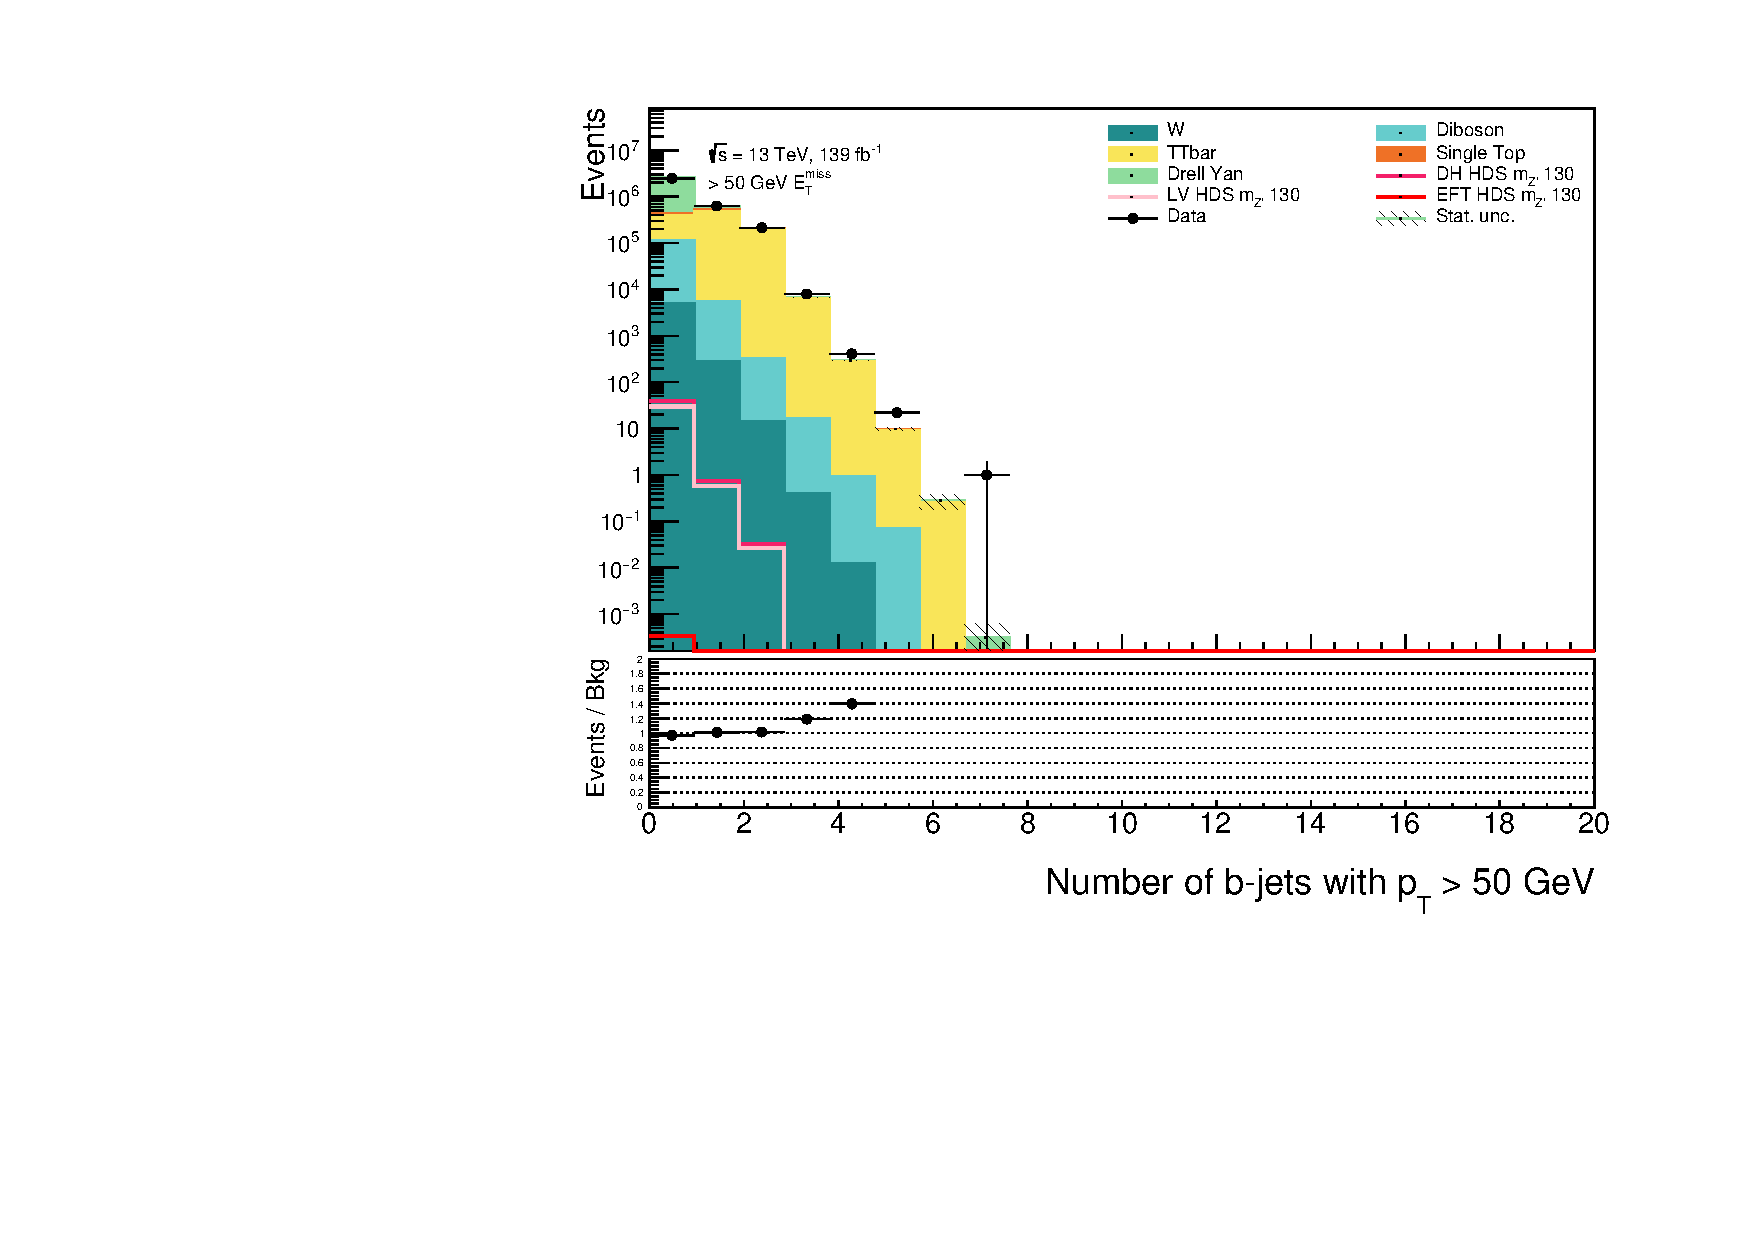
\includegraphics[width=\textwidth]{bjetsPt50.pdf}
%     \end{subfigure}
%     \hfill\begin{subfigure}[b]{0.49\textwidth}
%         \centering
%         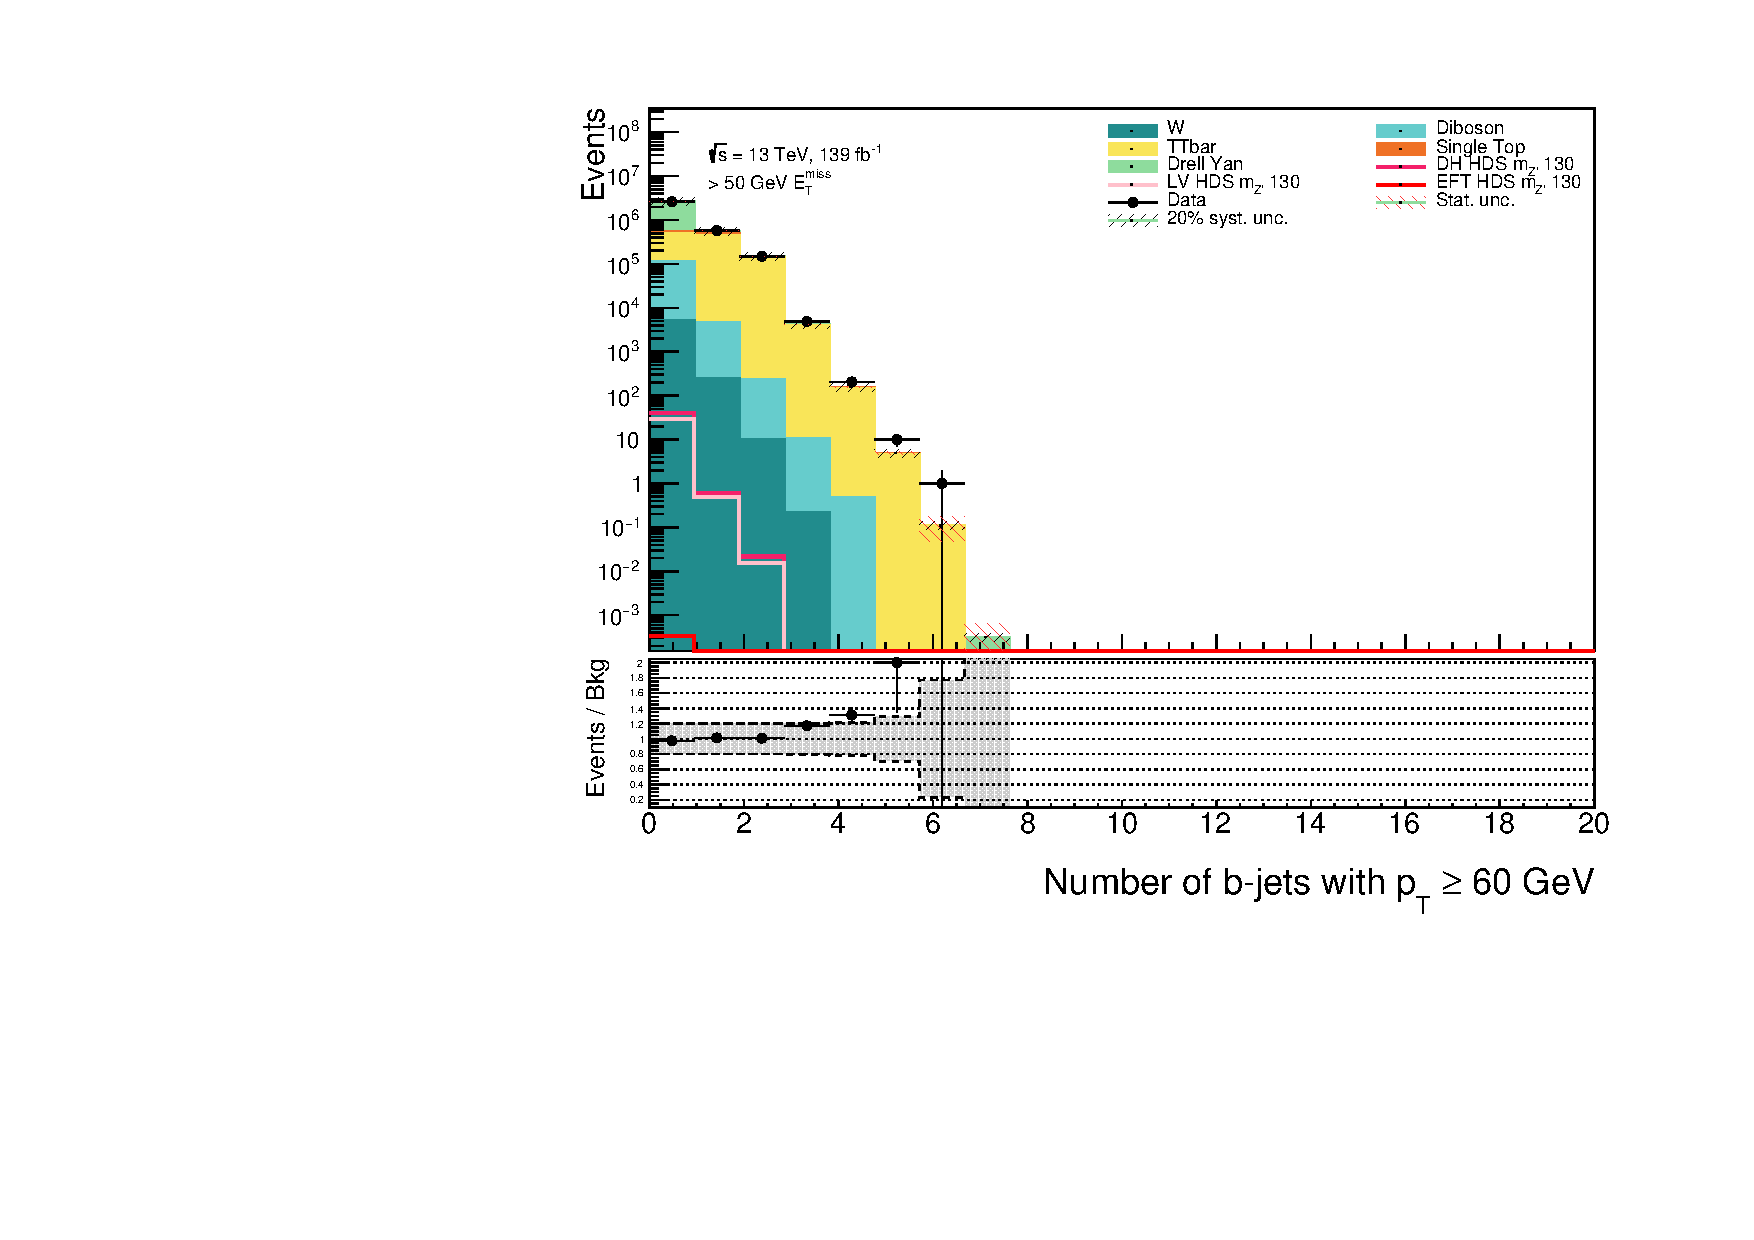
\includegraphics[width=\textwidth]{bjetsPt60.pdf}
%     \end{subfigure}
%     \caption{Data and MC agreement on number of b- jets with different $p_T$ cuts on full Run II.}
% \end{figure}

% \begin{figure}[!ht]
%     \centering
%     \begin{subfigure}[b]{0.49\textwidth}
%         \centering
%         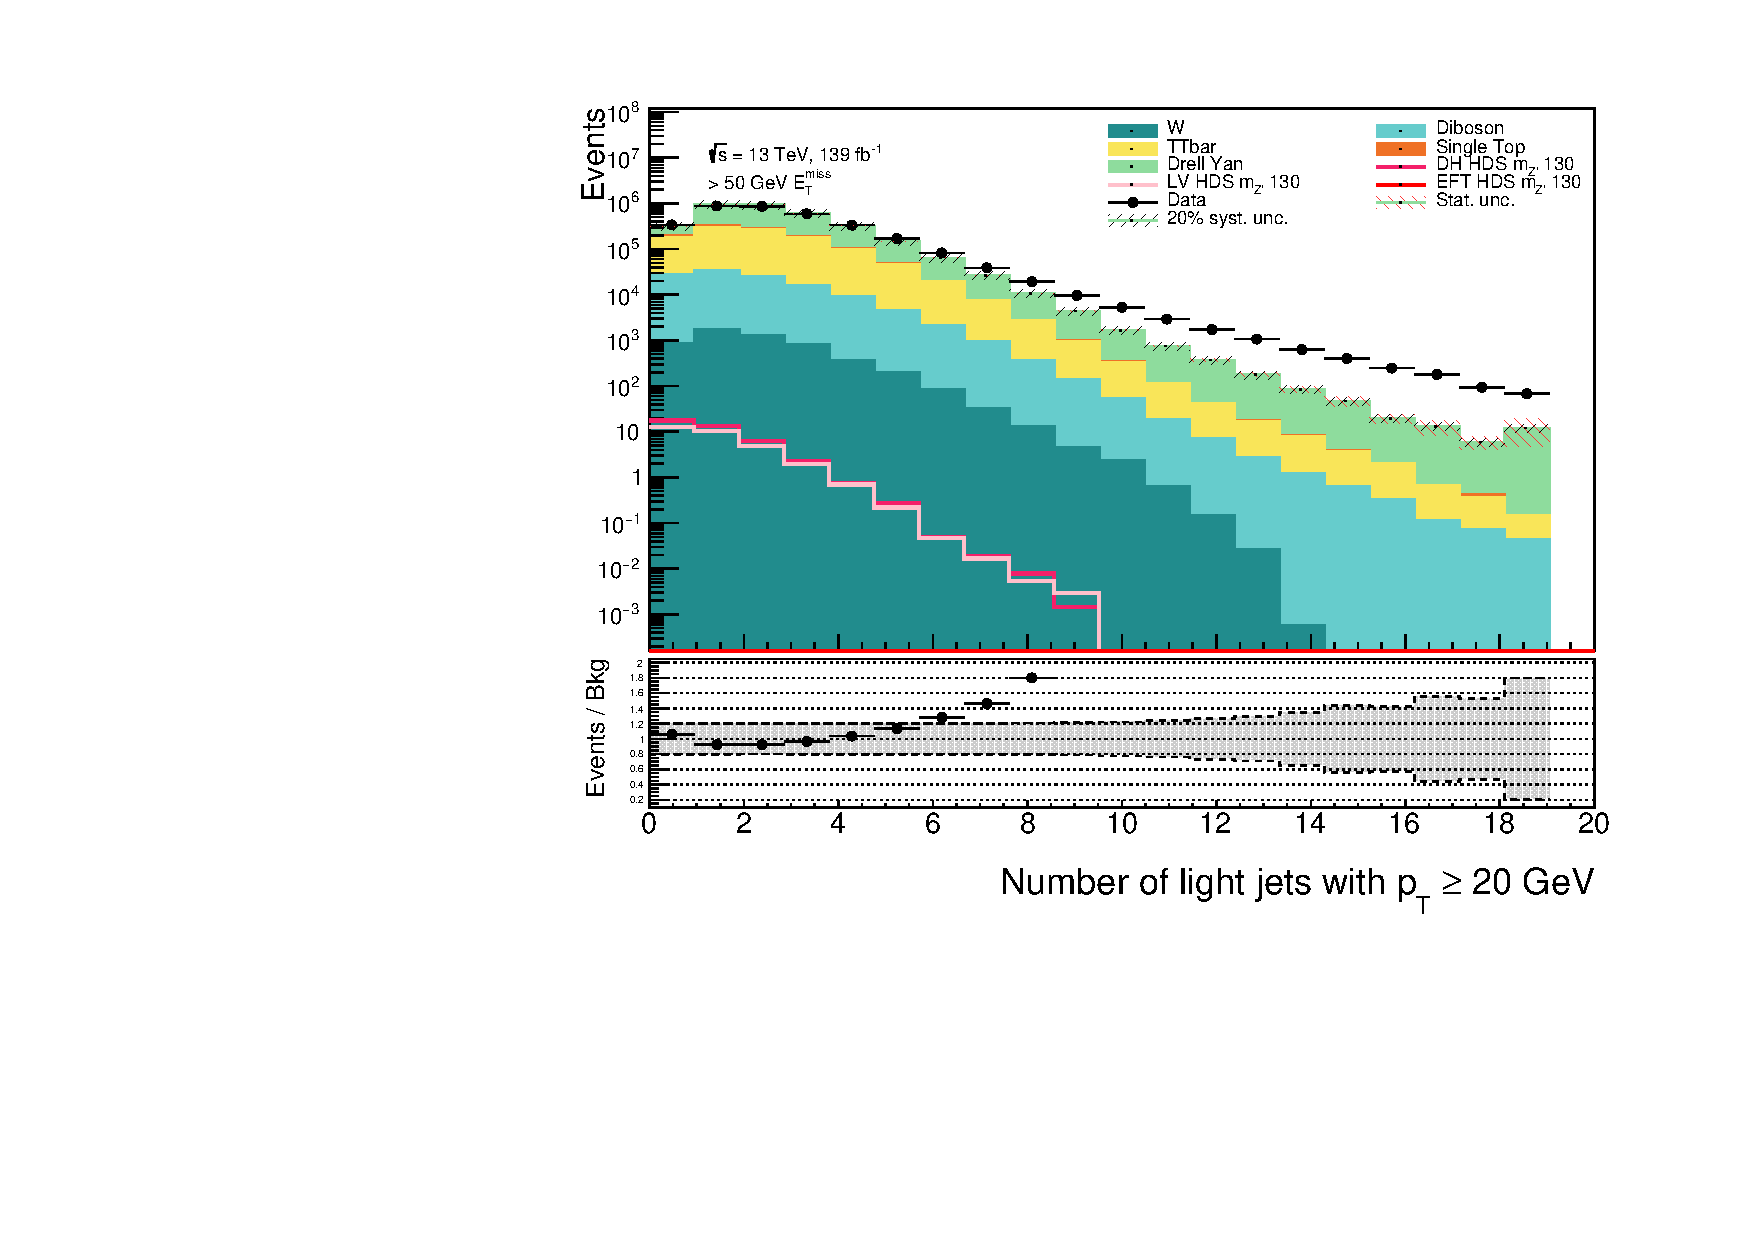
\includegraphics[width=\textwidth]{ljetsPt20.pdf}
%     \end{subfigure}
%     \hfill\begin{subfigure}[b]{0.49\textwidth}
%         \centering
%         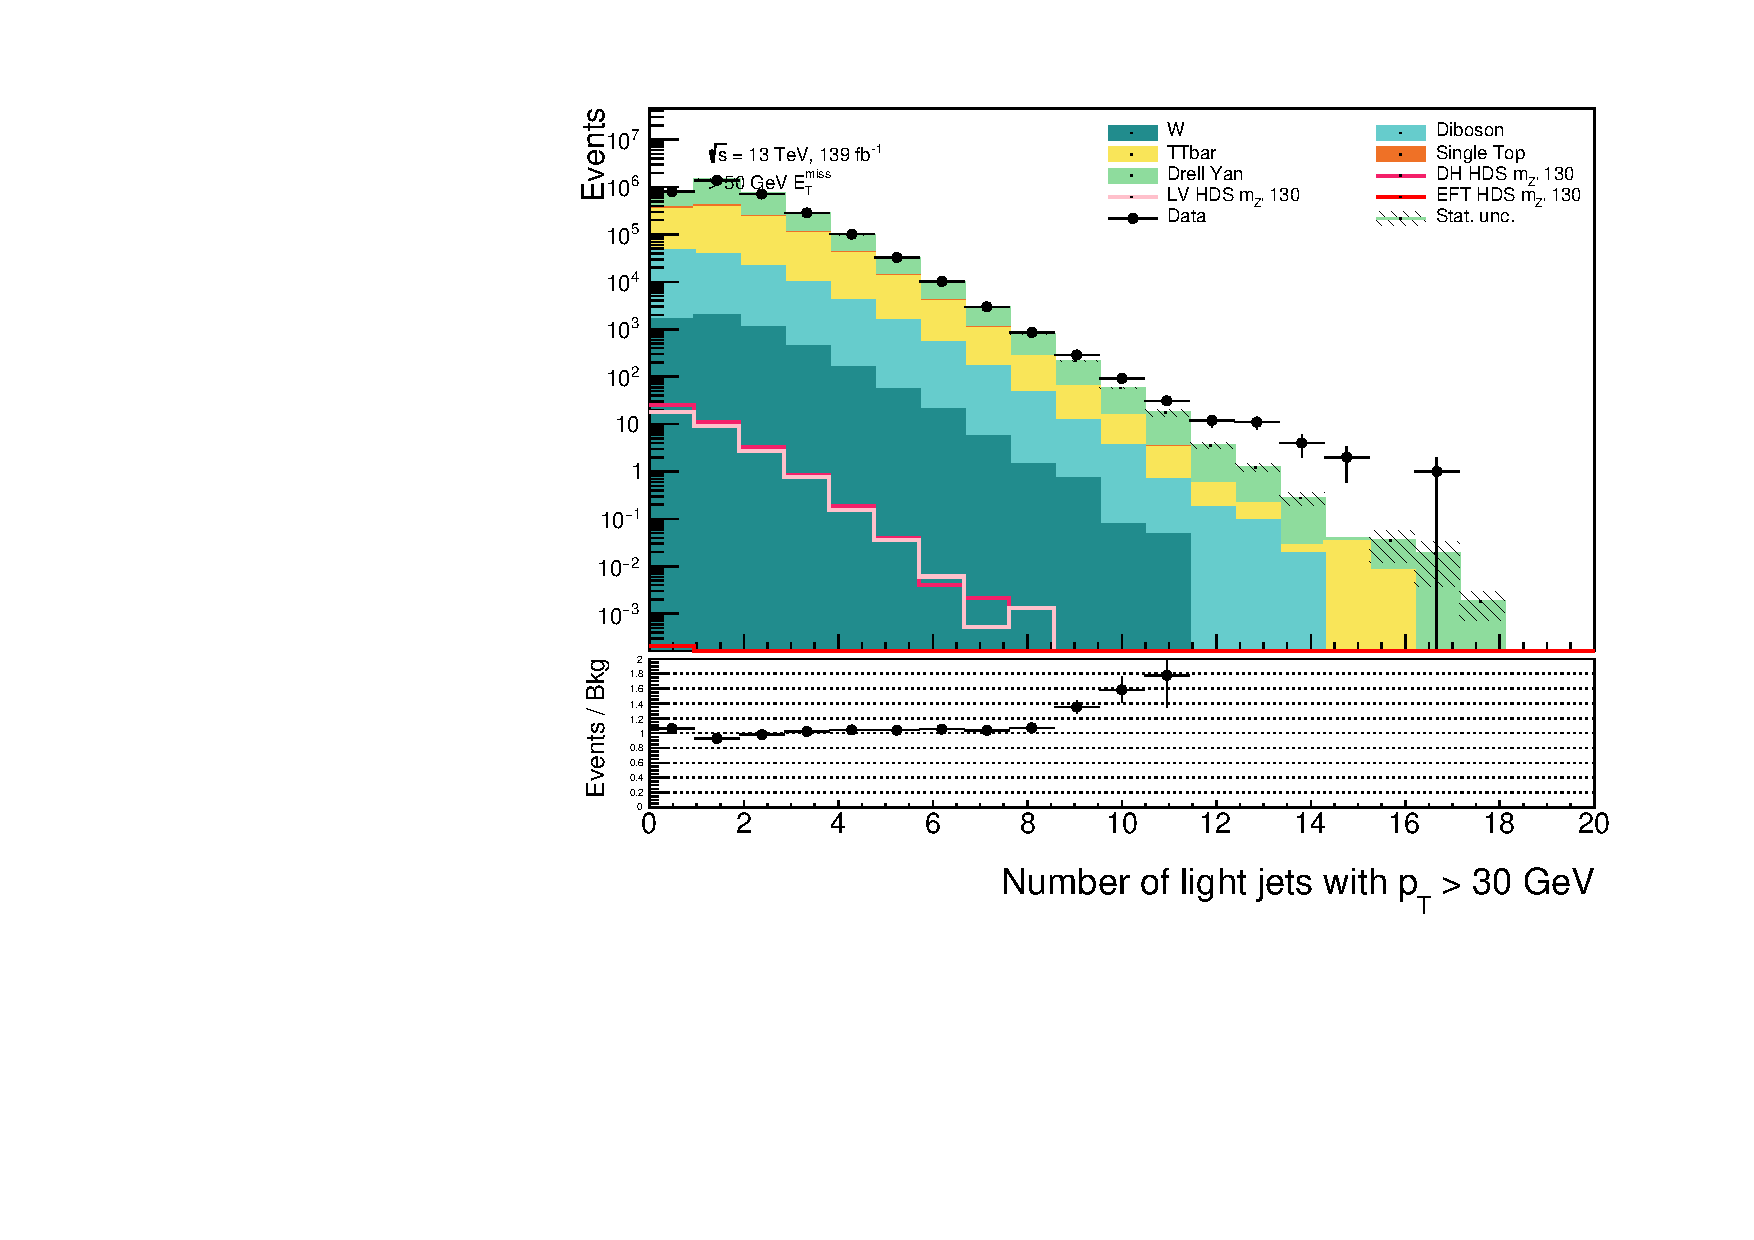
\includegraphics[width=\textwidth]{ljetsPt30.pdf}
%     \end{subfigure}
%     \hfill\begin{subfigure}[b]{0.49\textwidth}
%         \centering
%         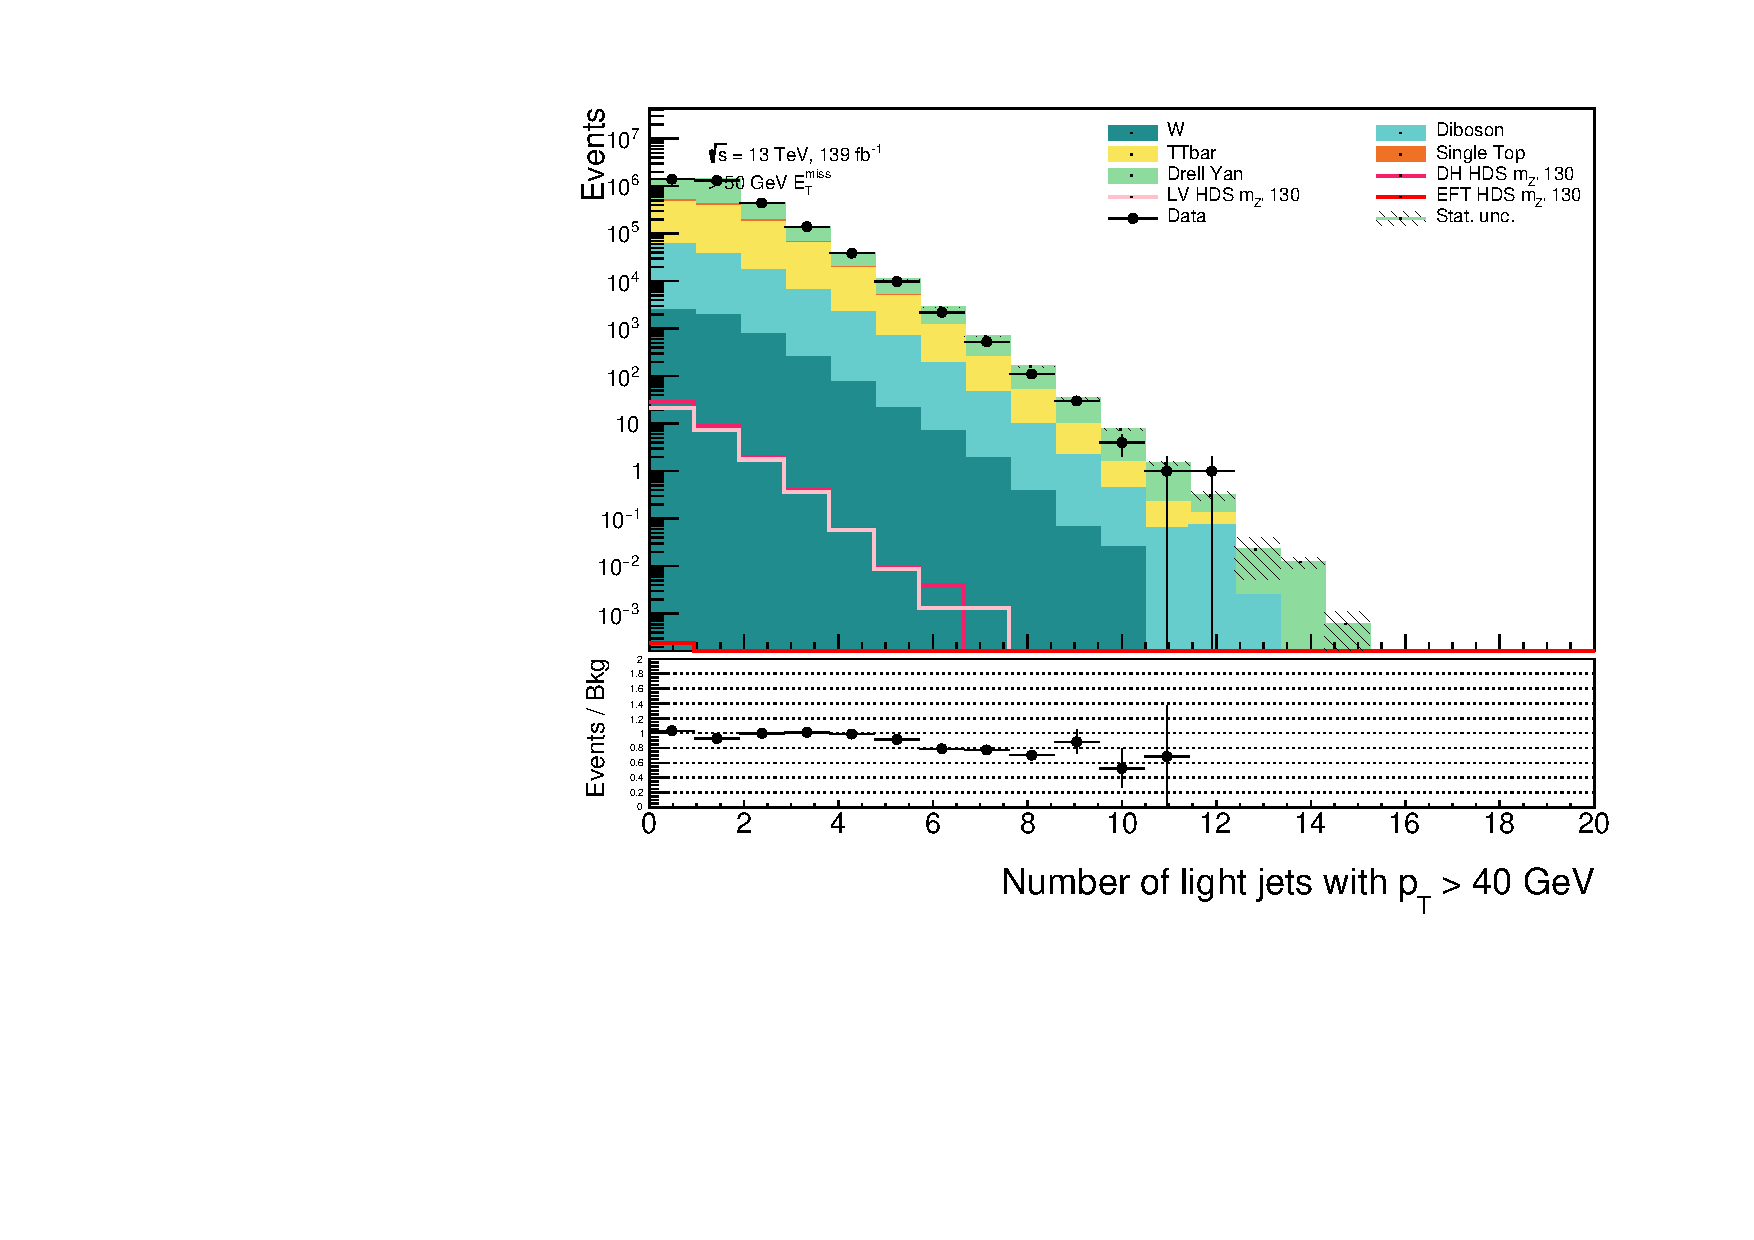
\includegraphics[width=\textwidth]{ljetsPt40.pdf}
%     \end{subfigure}
%     \hfill\begin{subfigure}[b]{0.49\textwidth}
%         \centering
%         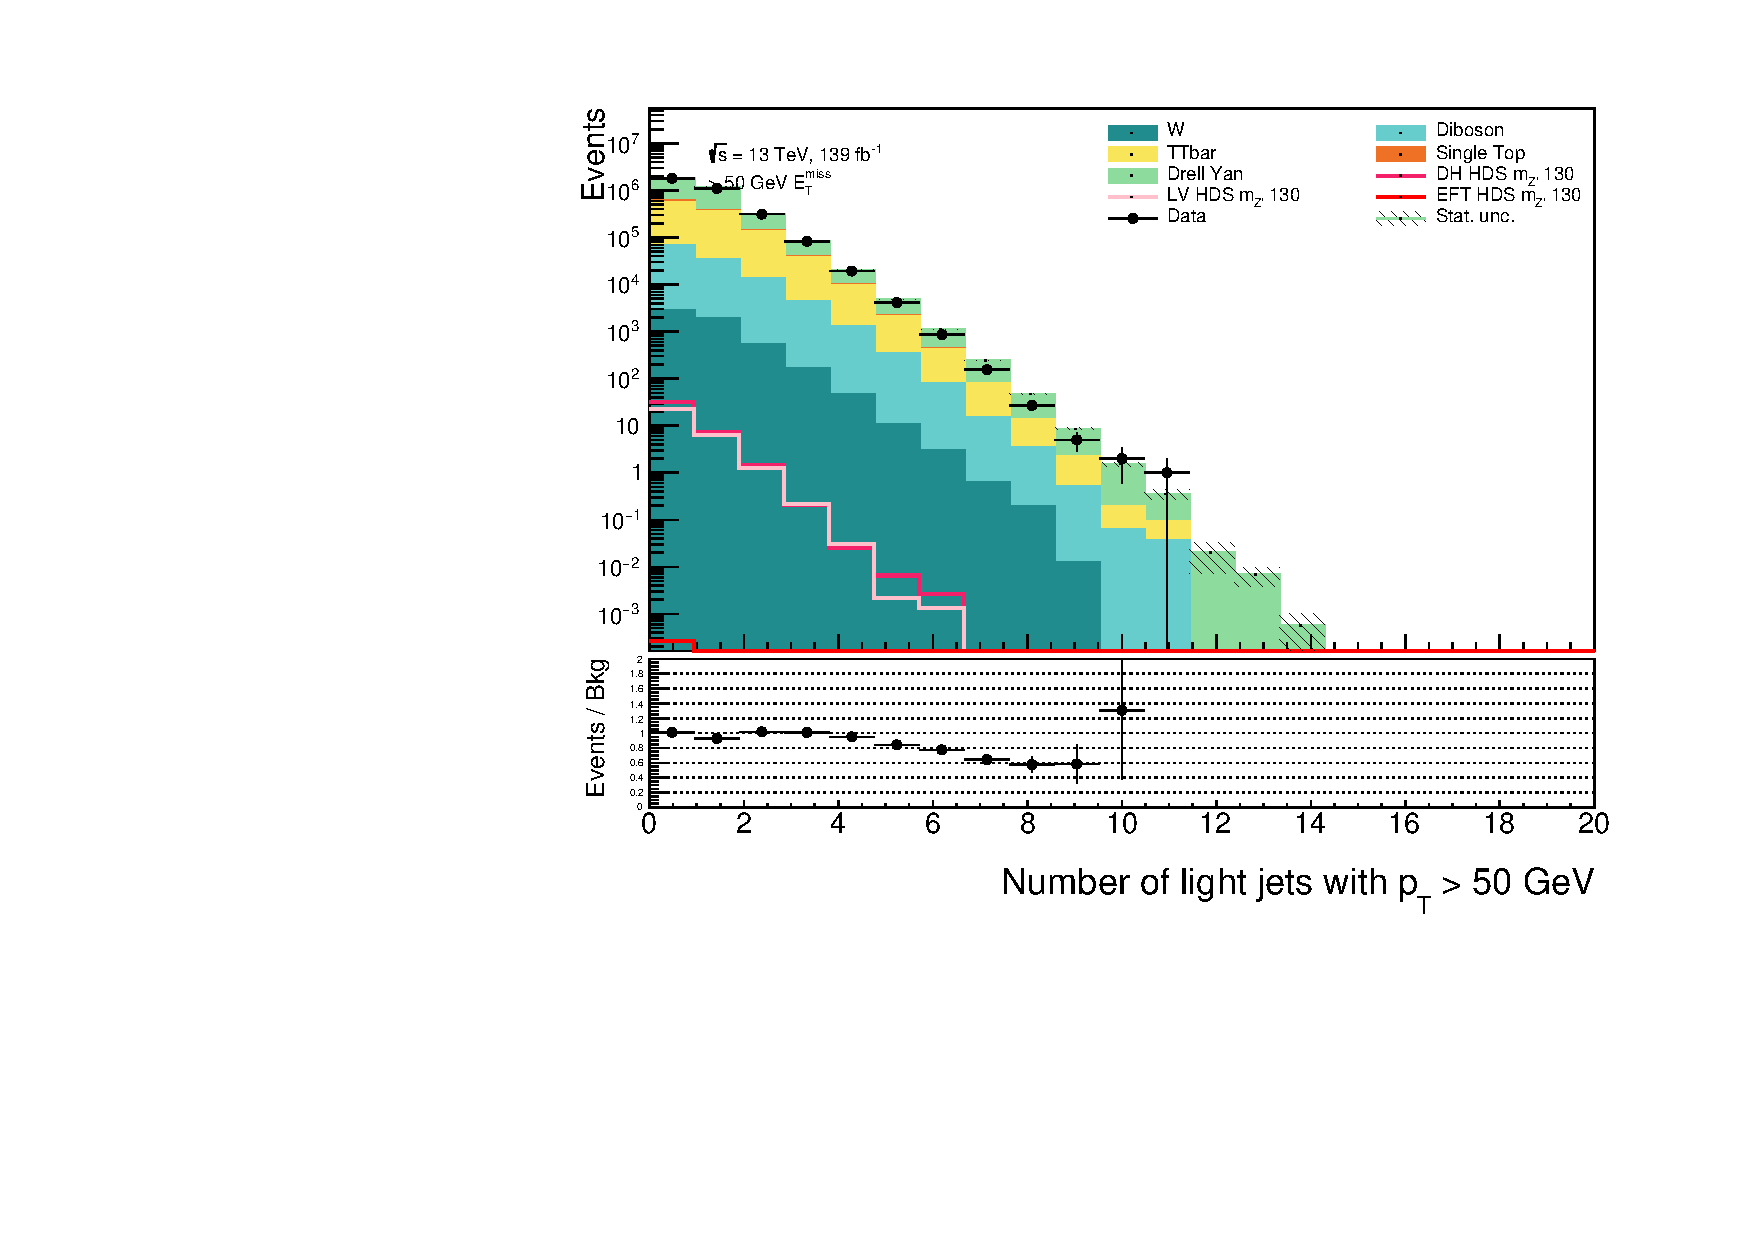
\includegraphics[width=\textwidth]{ljetsPt50.pdf}
%     \end{subfigure}
%     \hfill\begin{subfigure}[b]{0.49\textwidth}
%         \centering
%         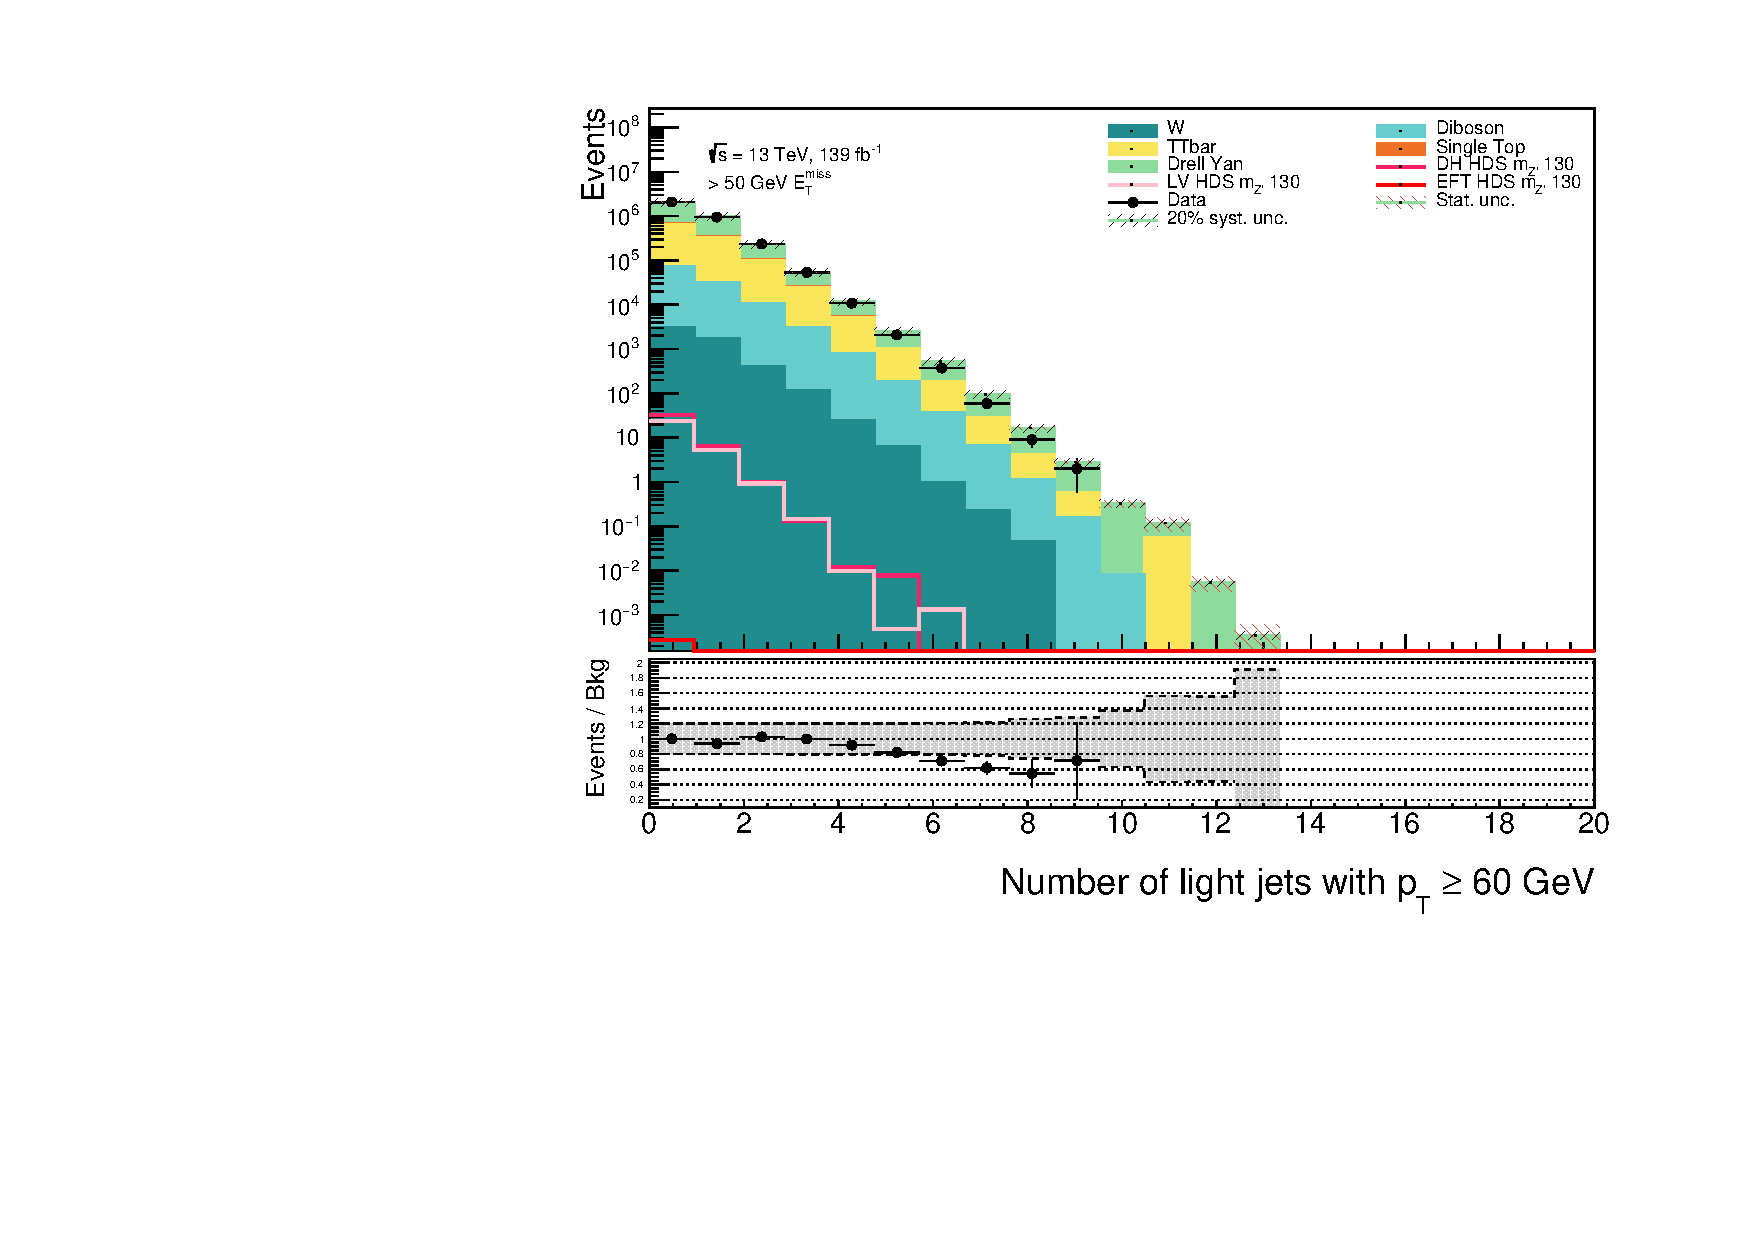
\includegraphics[width=\textwidth]{ljetsPt60.pdf}
%     \end{subfigure}
%     \caption{Data and MC agreement on number of light jets with different $p_T$ cuts on full Run II.}
% \end{figure}

% \graphicspath{{../../Plots/Data_Analysis/JetSelection/50-100_MET-120_mll/}} 
% \begin{figure}[!ht]
%     \centering
%     \begin{subfigure}[b]{0.49\textwidth}
%         \centering
%         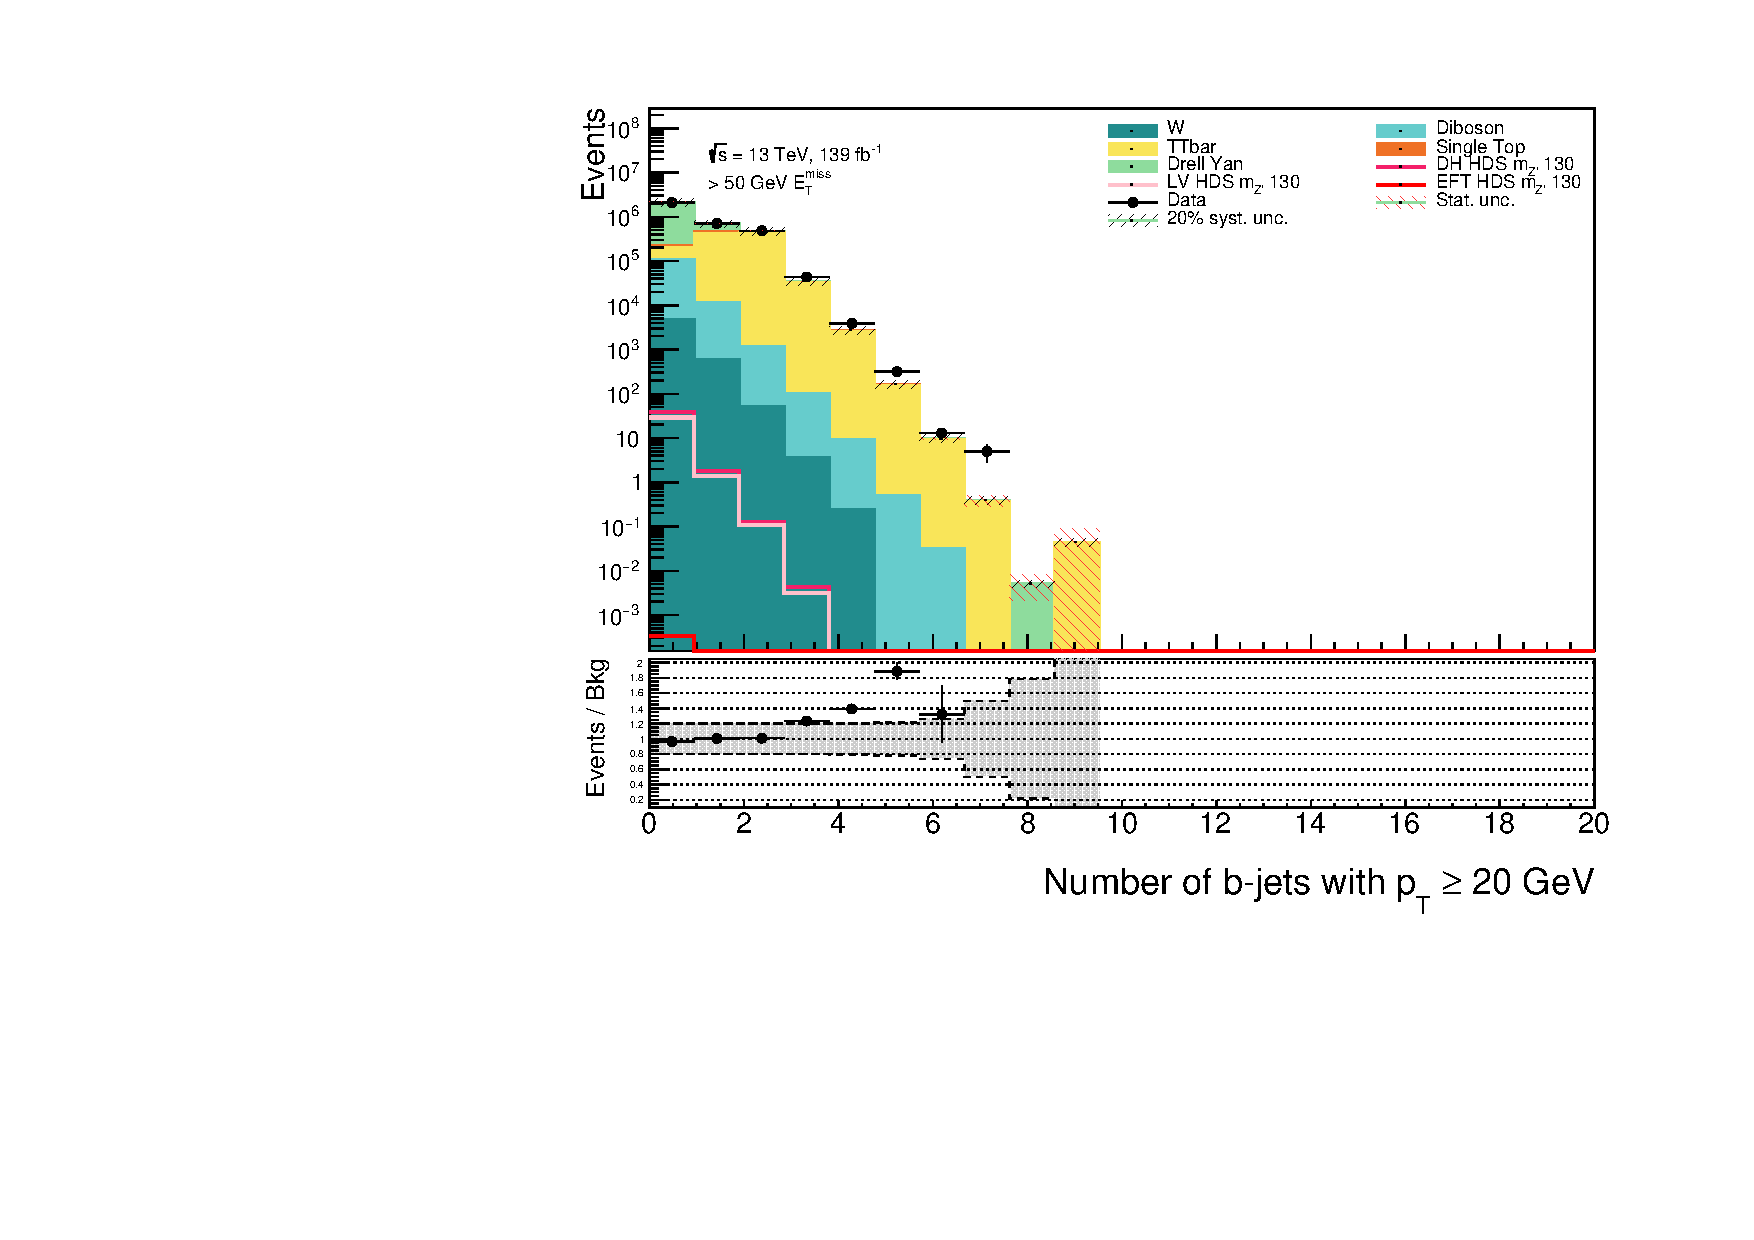
\includegraphics[width=\textwidth]{bjetsPt20.pdf}
%     \end{subfigure}
%     \hfill\begin{subfigure}[b]{0.49\textwidth}
%         \centering
%         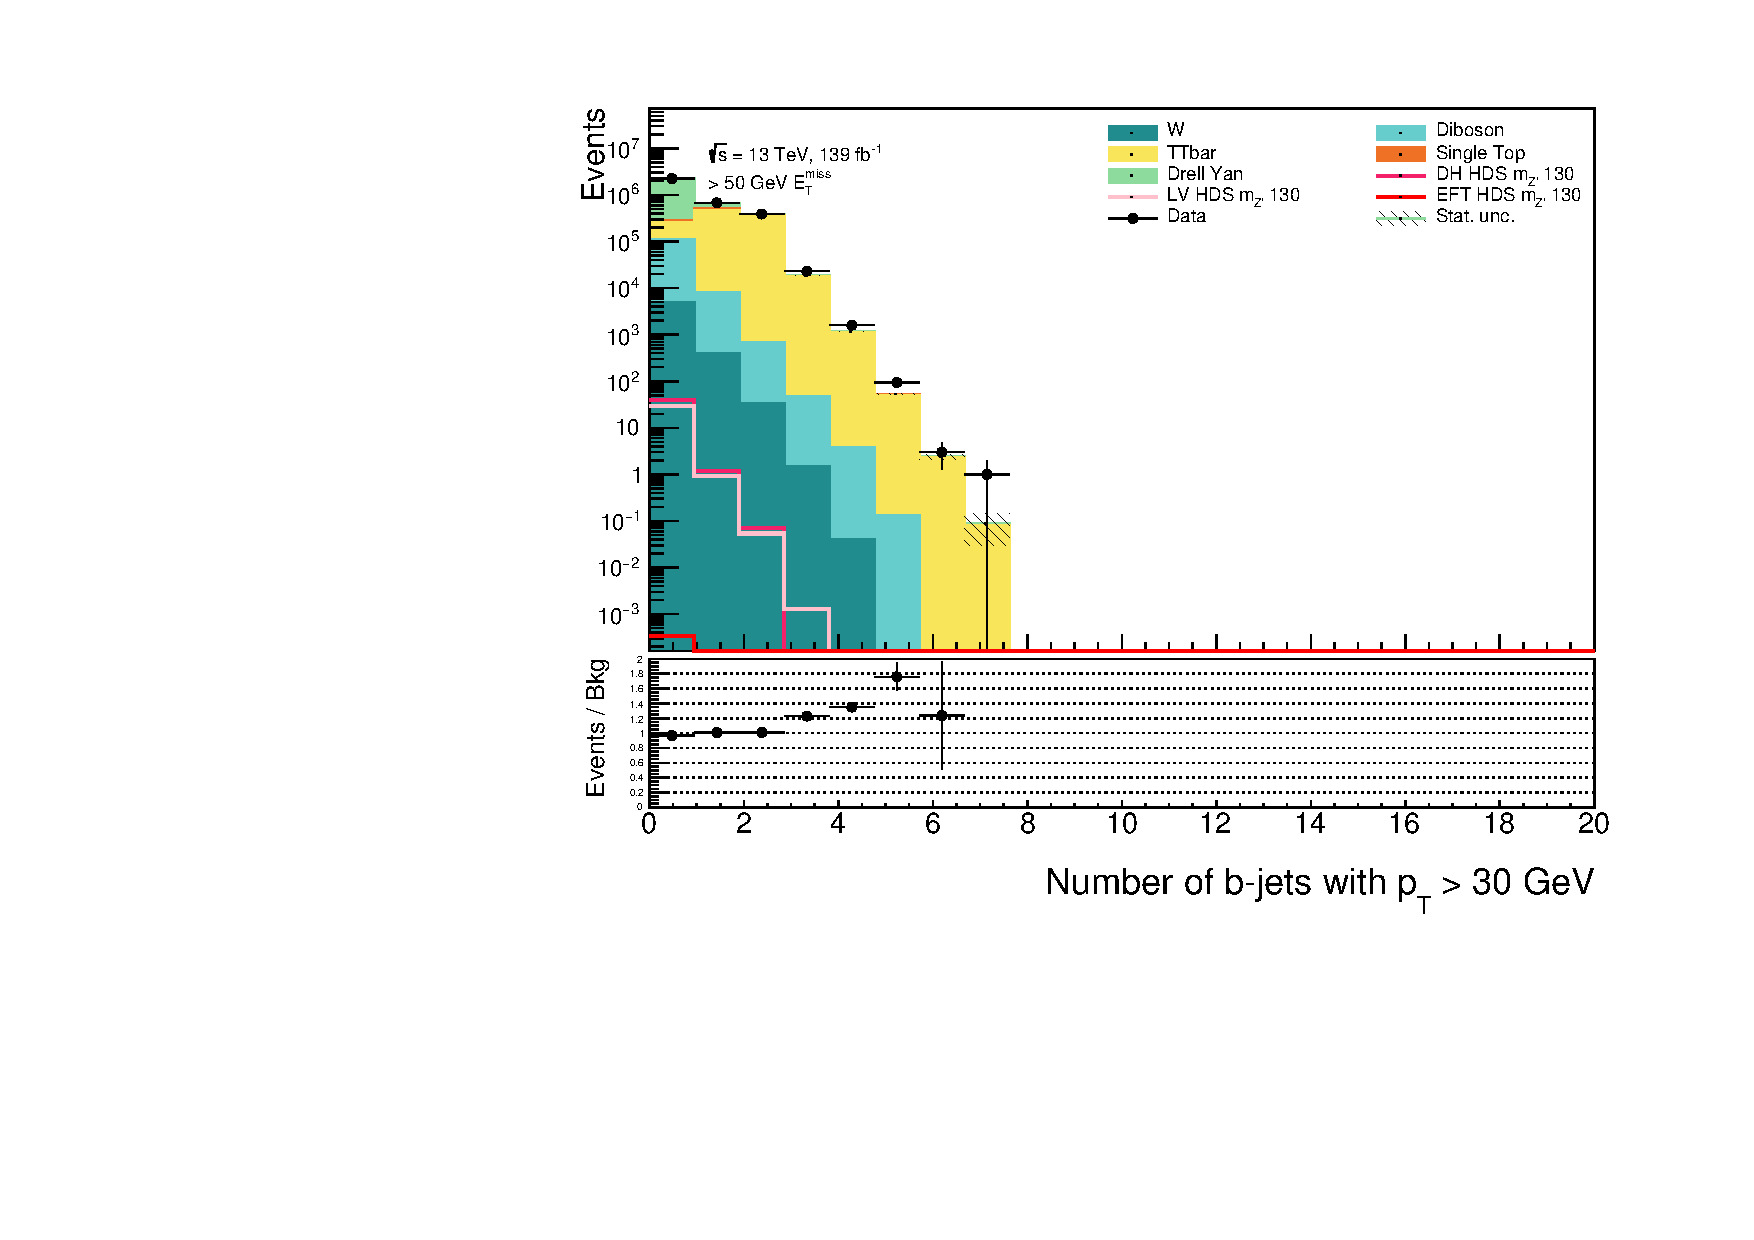
\includegraphics[width=\textwidth]{bjetsPt30.pdf}
%     \end{subfigure}
%     \hfill\begin{subfigure}[b]{0.49\textwidth}
%         \centering
%         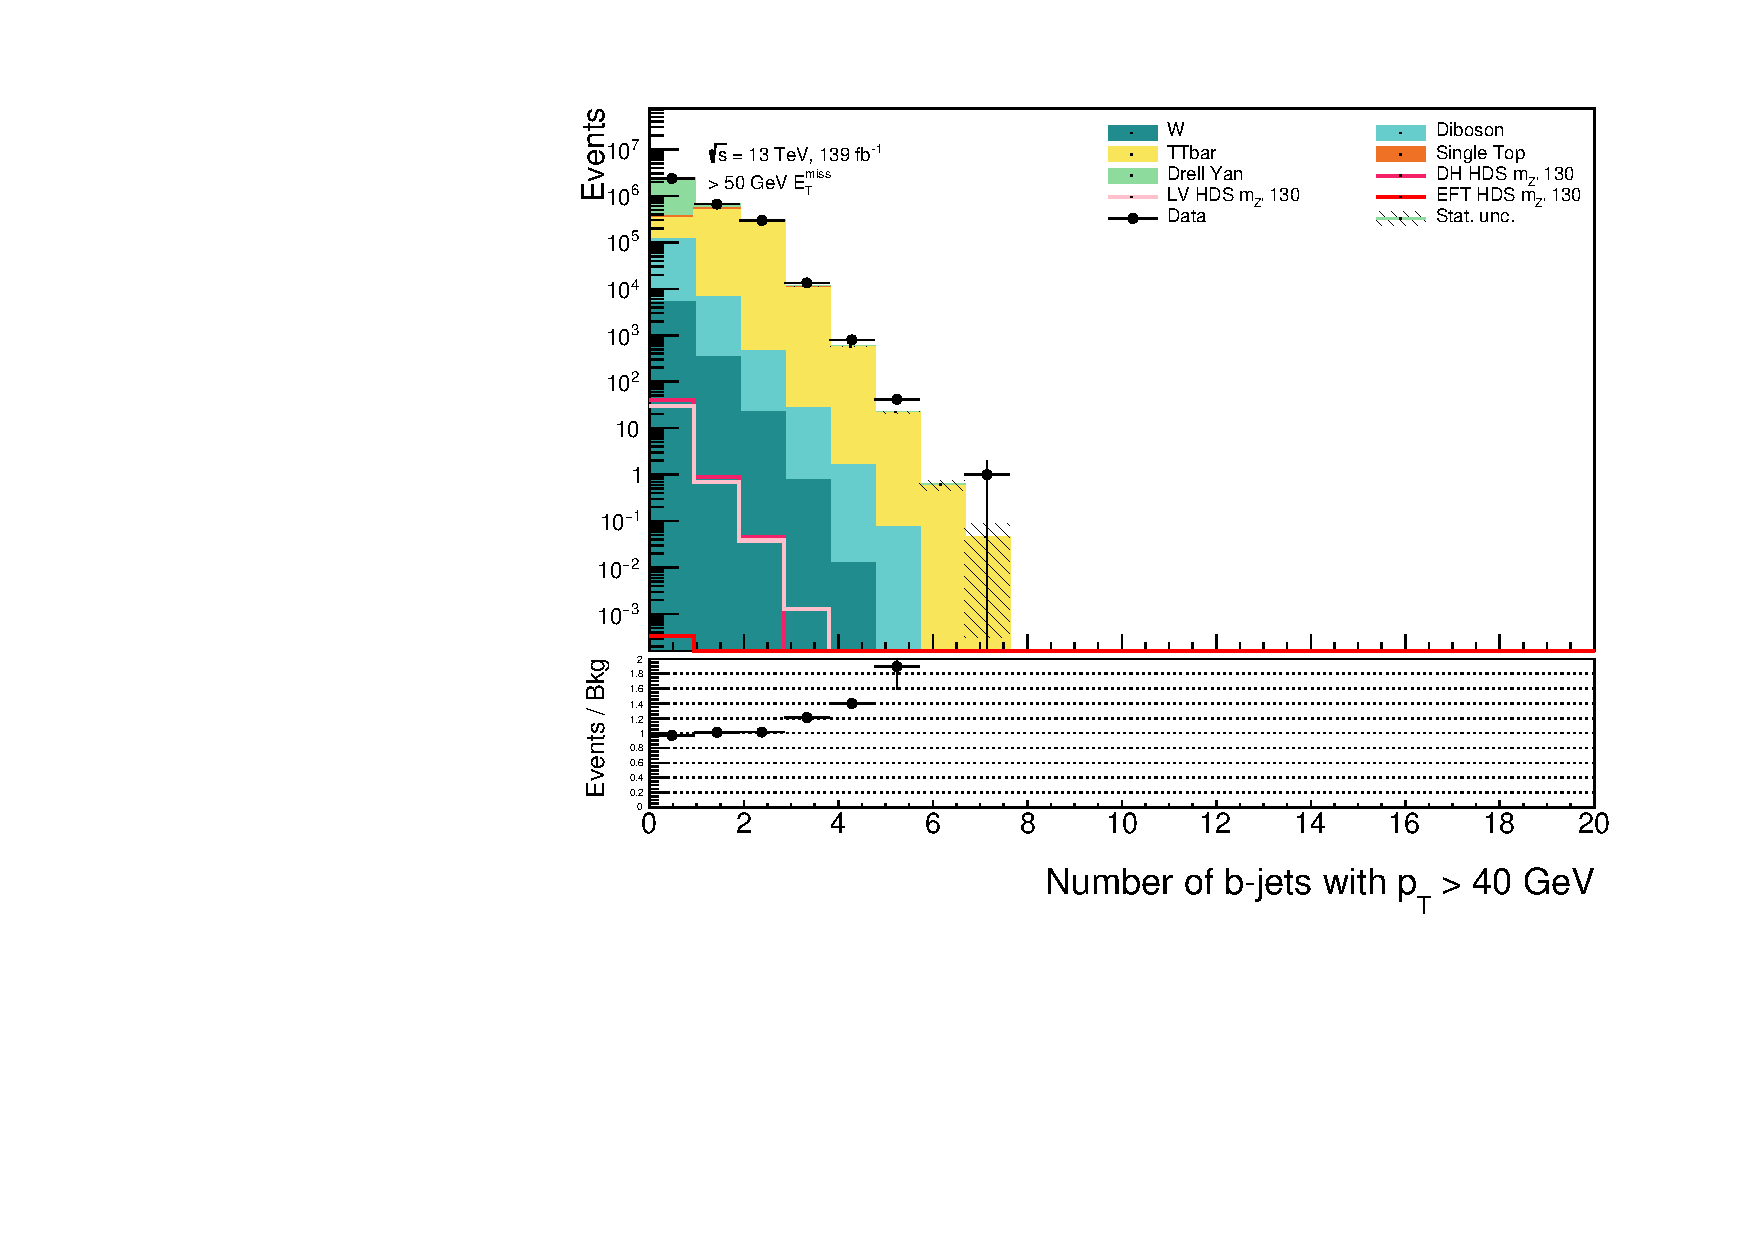
\includegraphics[width=\textwidth]{bjetsPt40.pdf}
%     \end{subfigure}
%     \hfill\begin{subfigure}[b]{0.49\textwidth}
%         \centering
%         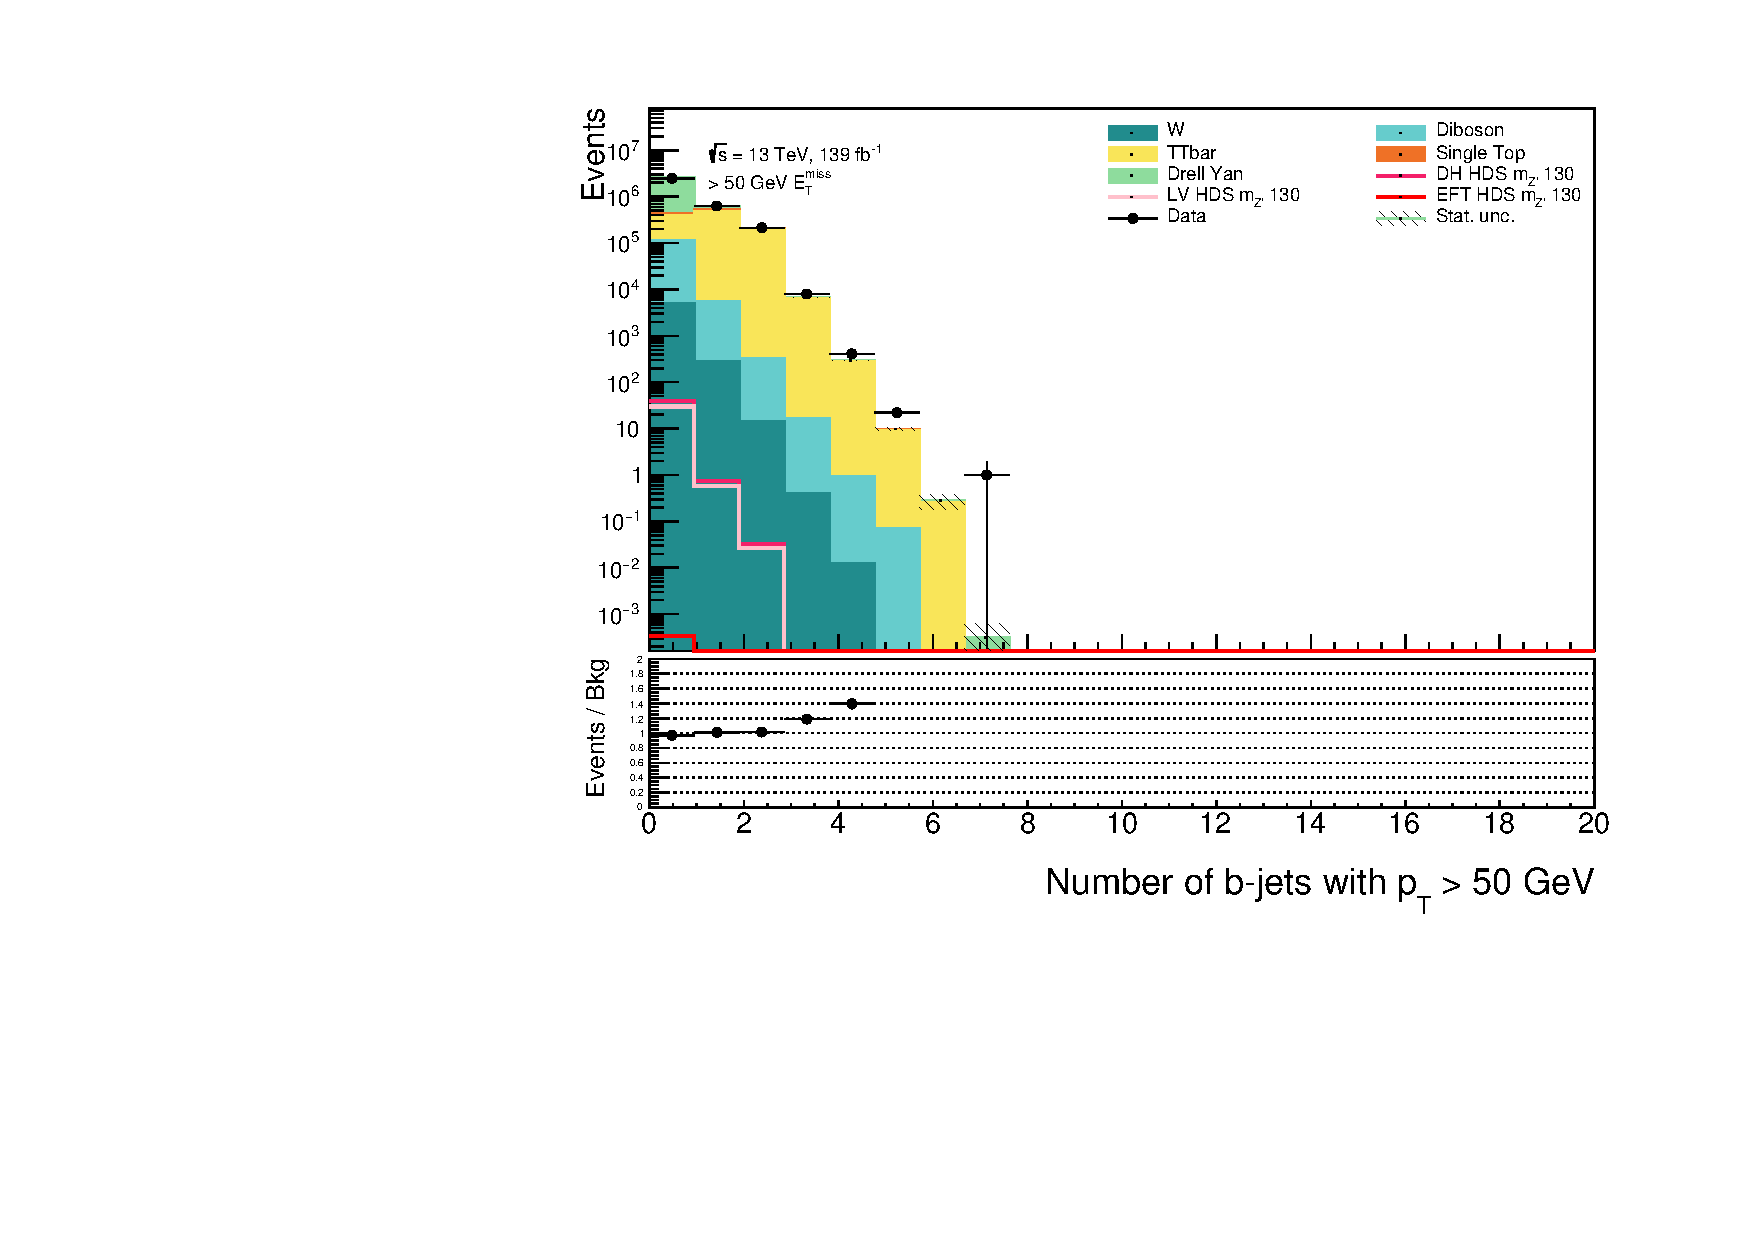
\includegraphics[width=\textwidth]{bjetsPt50.pdf}
%     \end{subfigure}
%     \hfill\begin{subfigure}[b]{0.49\textwidth}
%         \centering
%         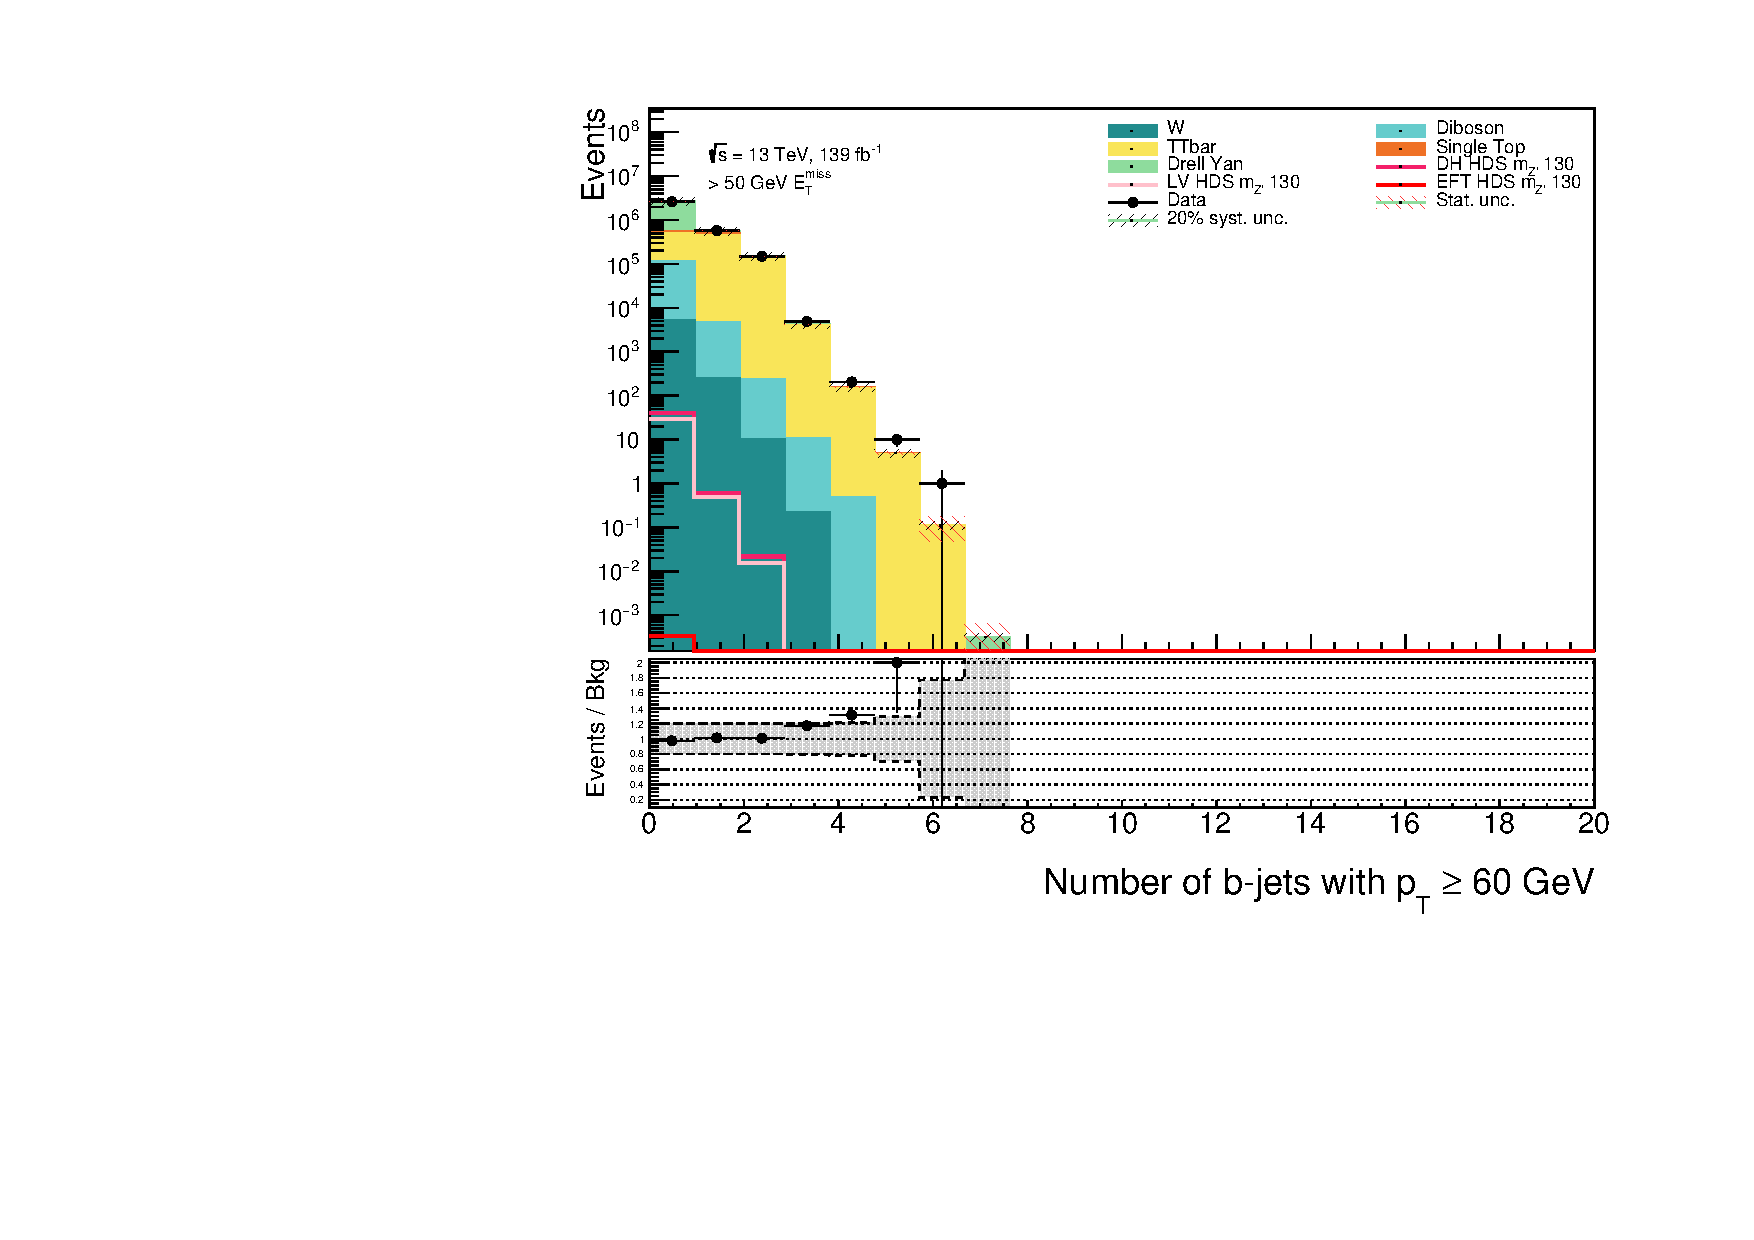
\includegraphics[width=\textwidth]{bjetsPt60.pdf}
%     \end{subfigure}
%     \caption{Data and MC agreement on number of b- jets with different $p_T$ cuts in SR1.}
% \end{figure}

% \begin{figure}[!ht]
%     \centering
%     \begin{subfigure}[b]{0.49\textwidth}
%         \centering
%         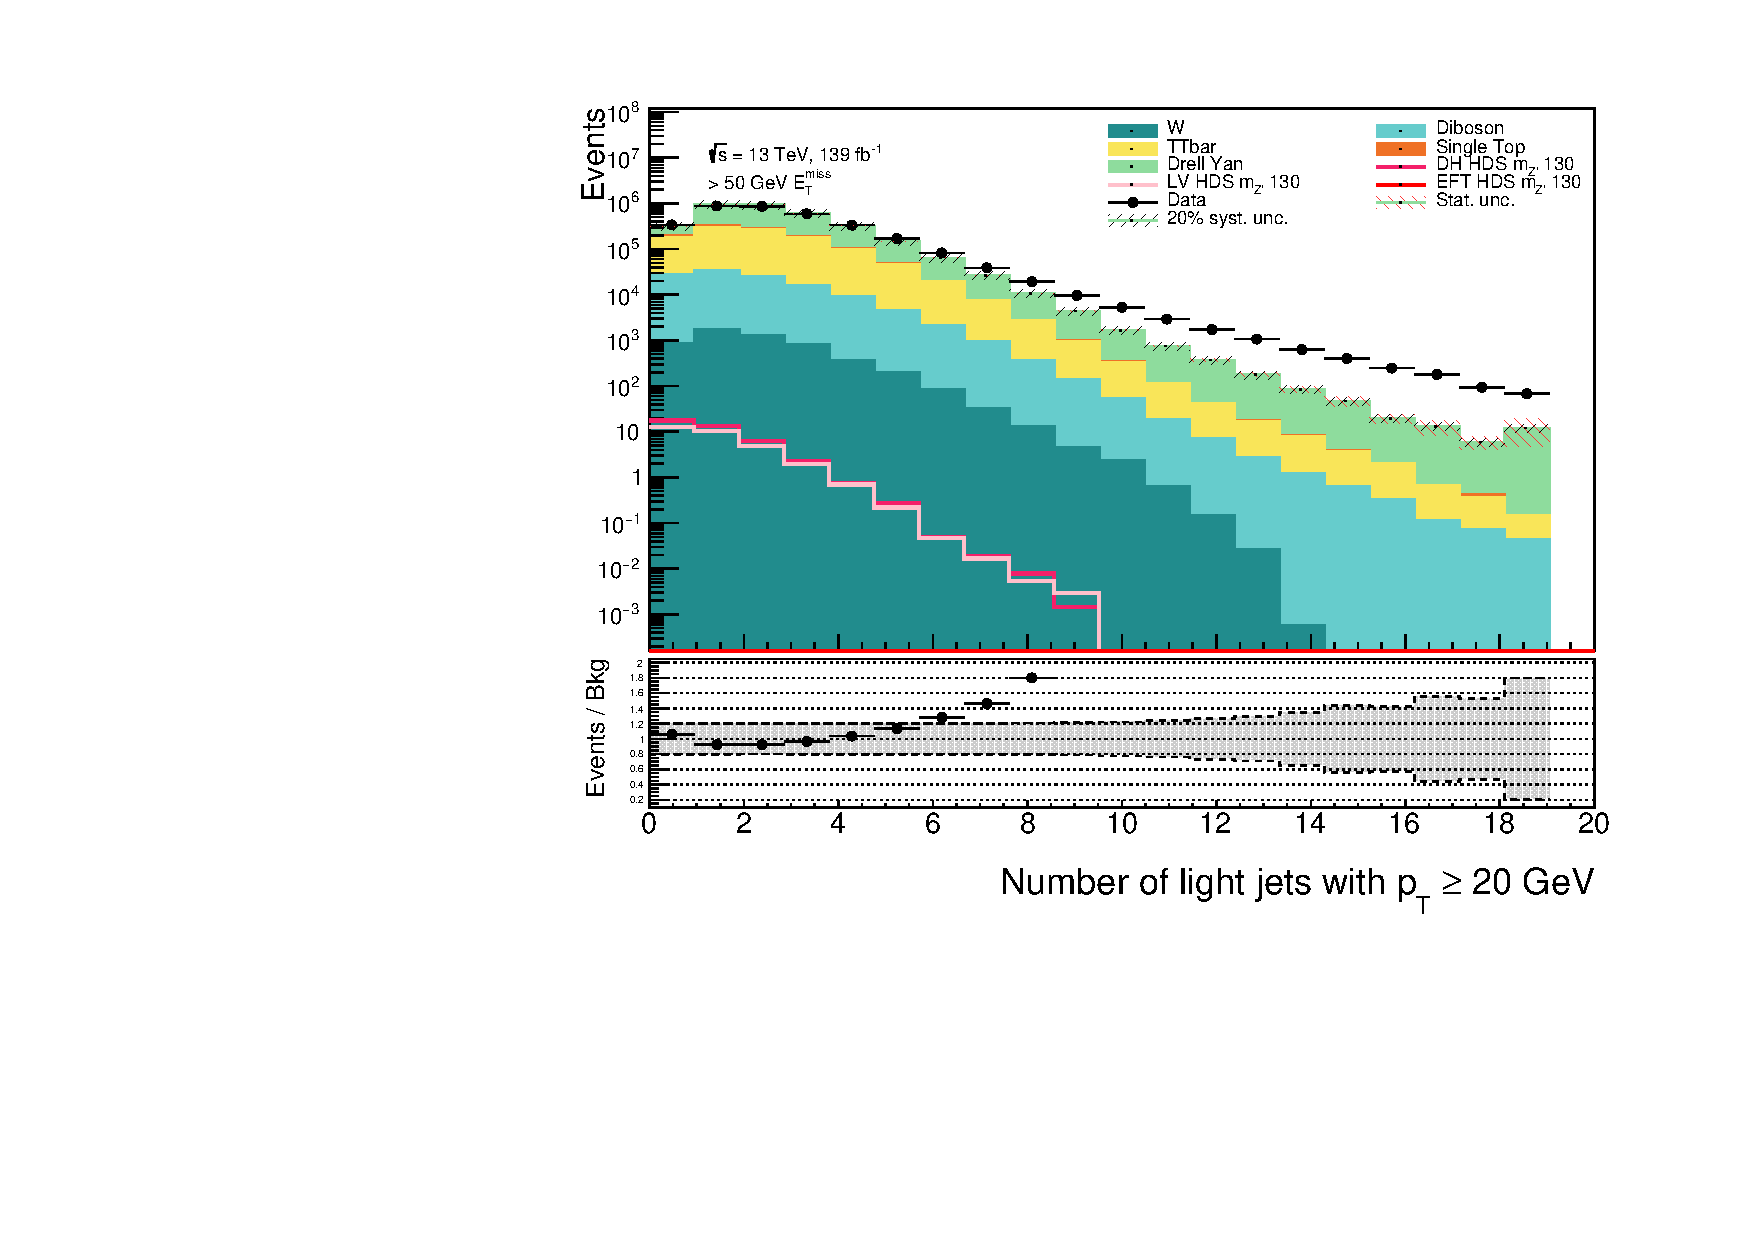
\includegraphics[width=\textwidth]{ljetsPt20.pdf}
%     \end{subfigure}
%     \hfill\begin{subfigure}[b]{0.49\textwidth}
%         \centering
%         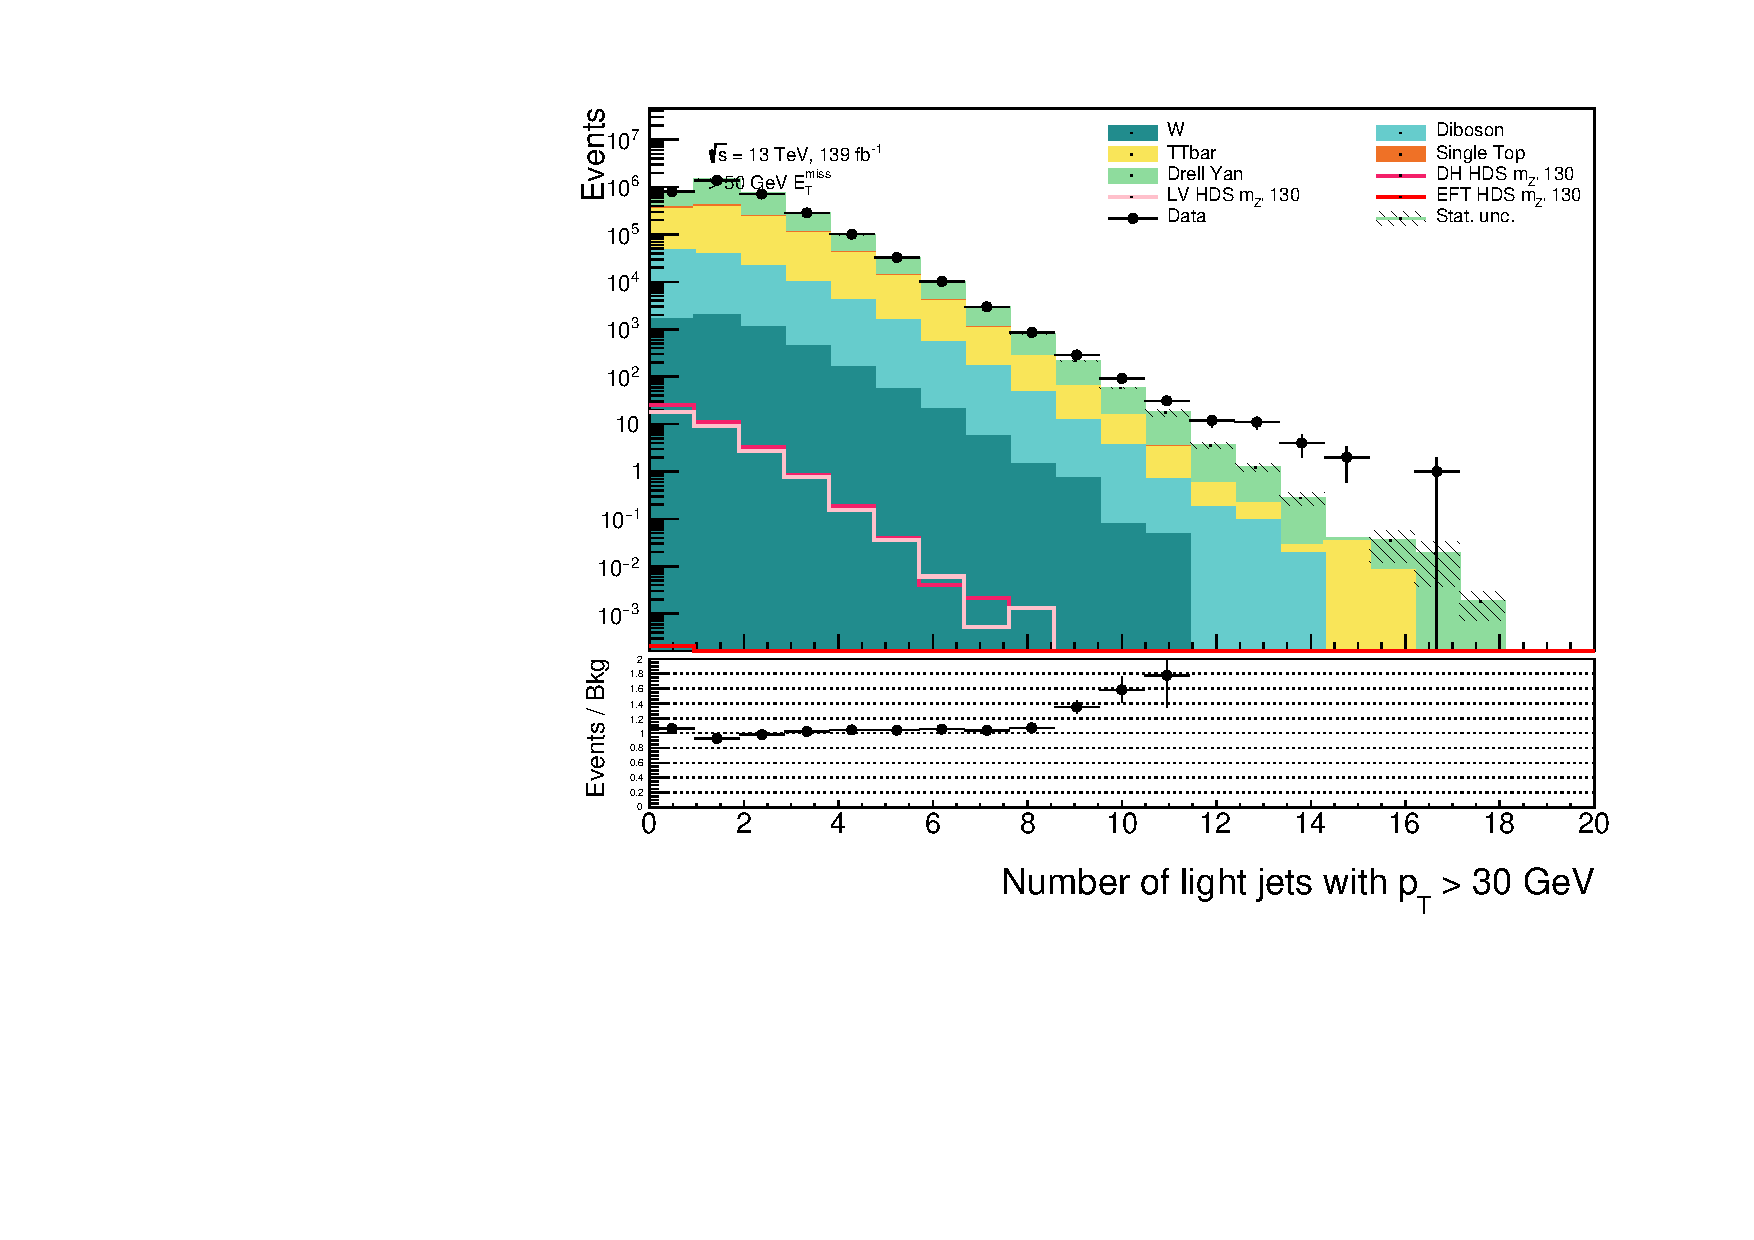
\includegraphics[width=\textwidth]{ljetsPt30.pdf}
%     \end{subfigure}
%     \hfill\begin{subfigure}[b]{0.49\textwidth}
%         \centering
%         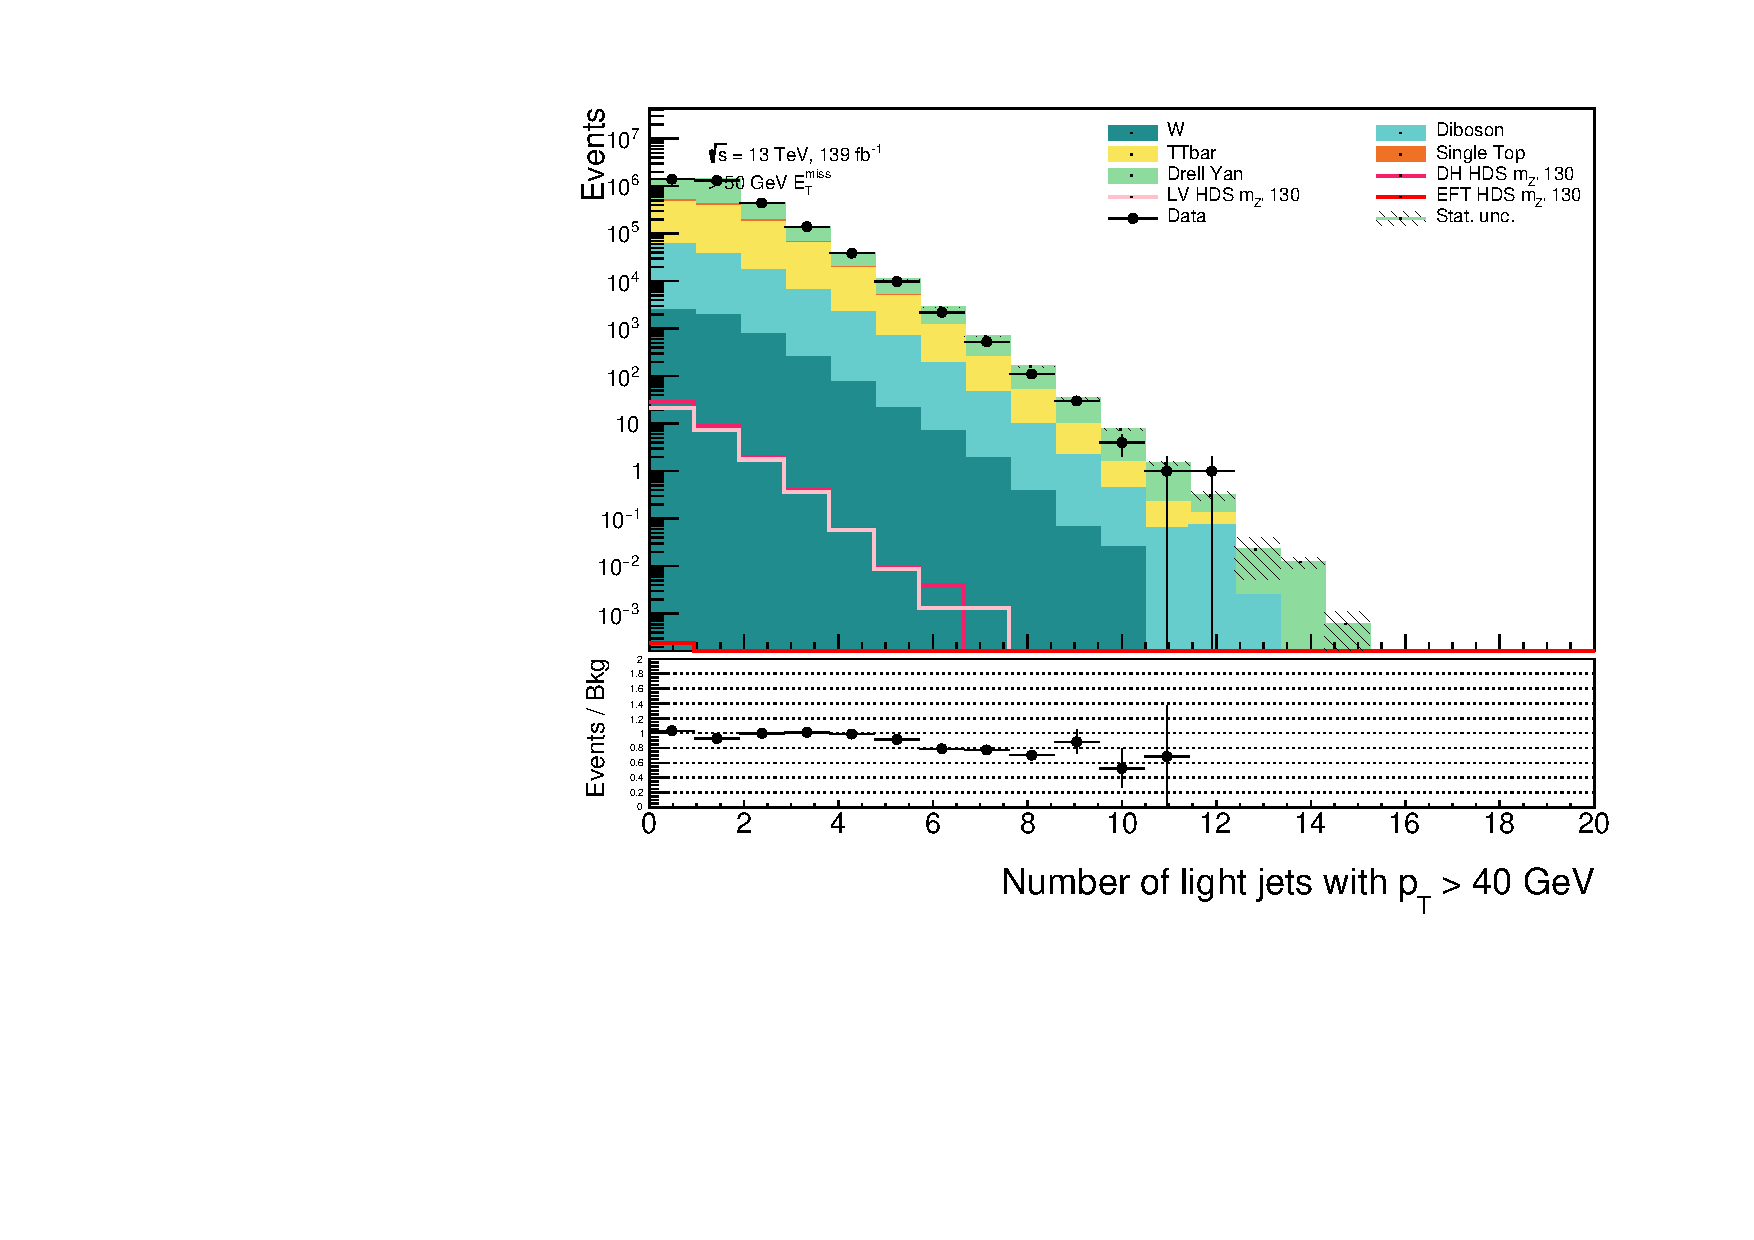
\includegraphics[width=\textwidth]{ljetsPt40.pdf}
%     \end{subfigure}
%     \hfill\begin{subfigure}[b]{0.49\textwidth}
%         \centering
%         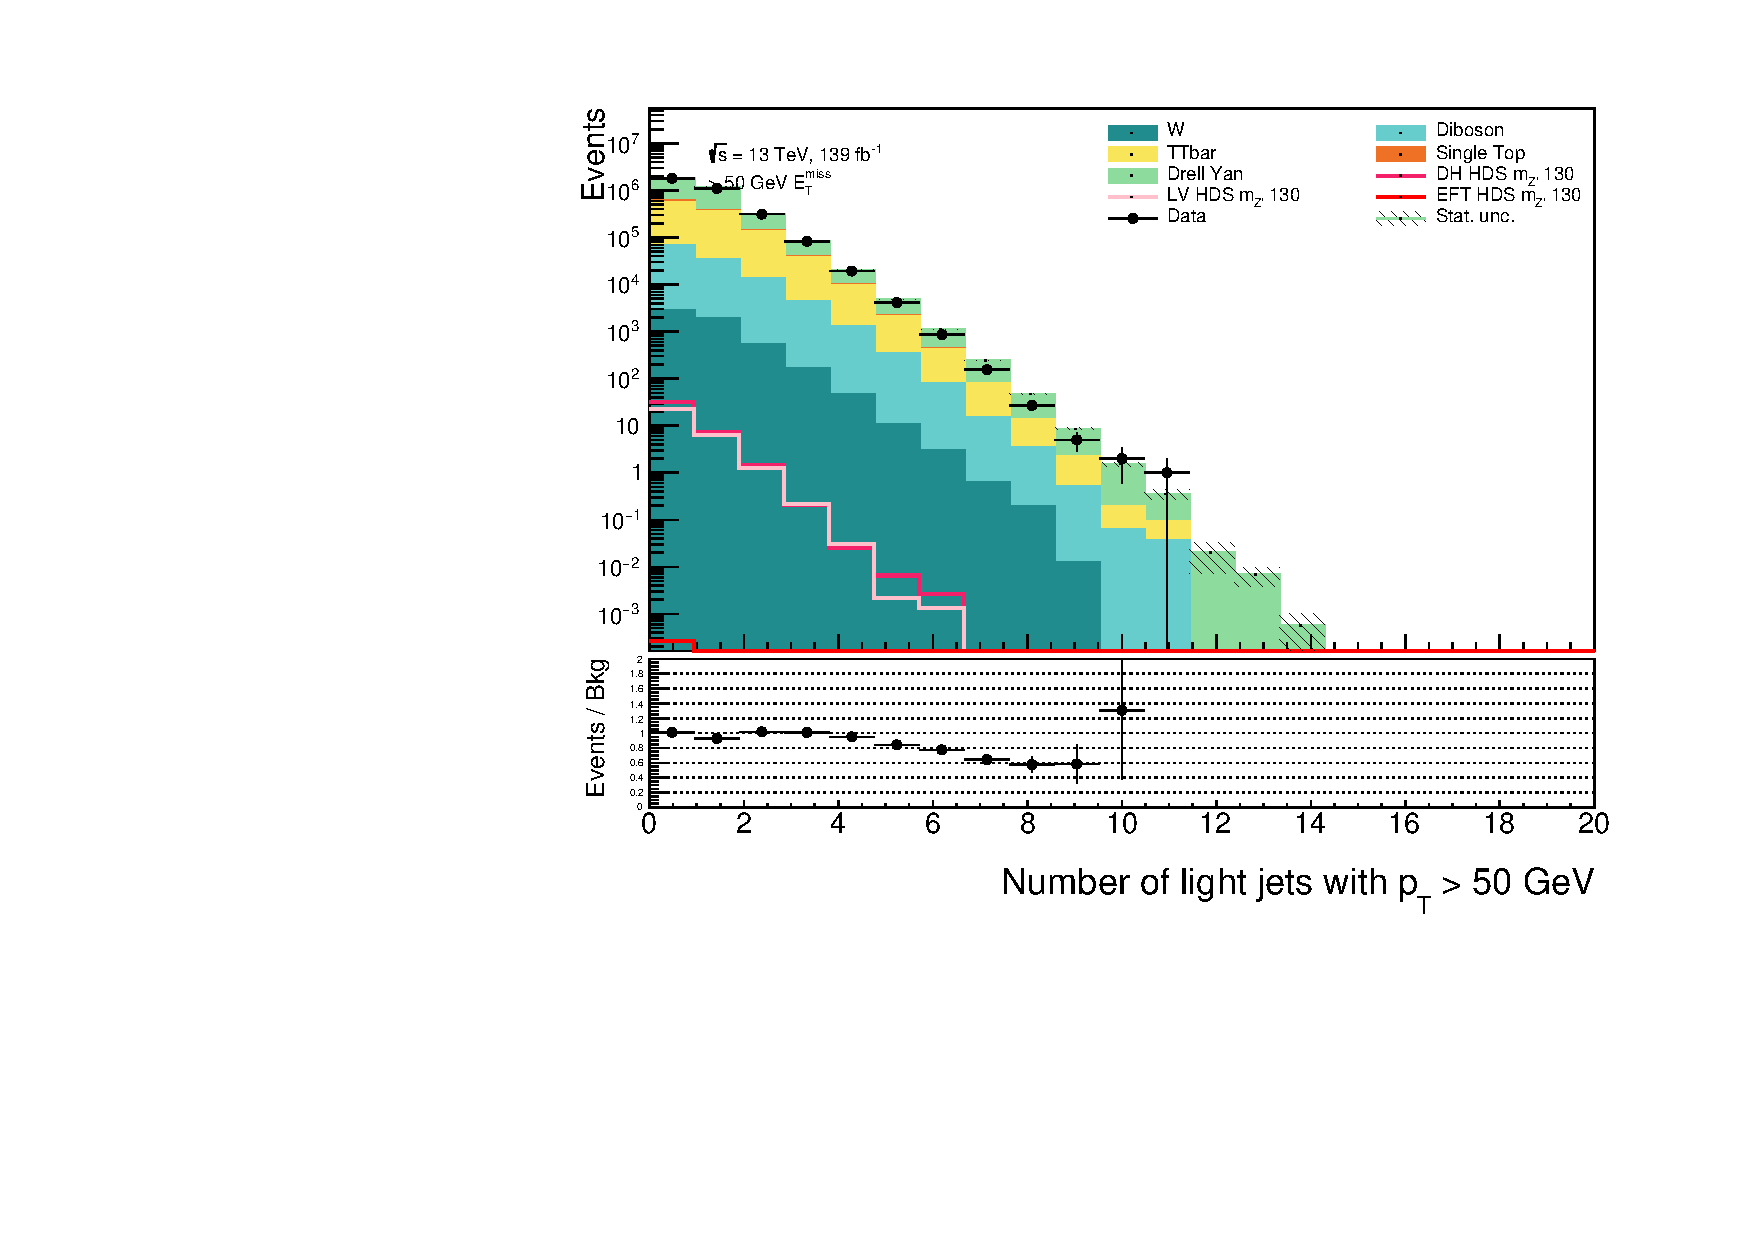
\includegraphics[width=\textwidth]{ljetsPt50.pdf}
%     \end{subfigure}
%     \hfill\begin{subfigure}[b]{0.49\textwidth}
%         \centering
%         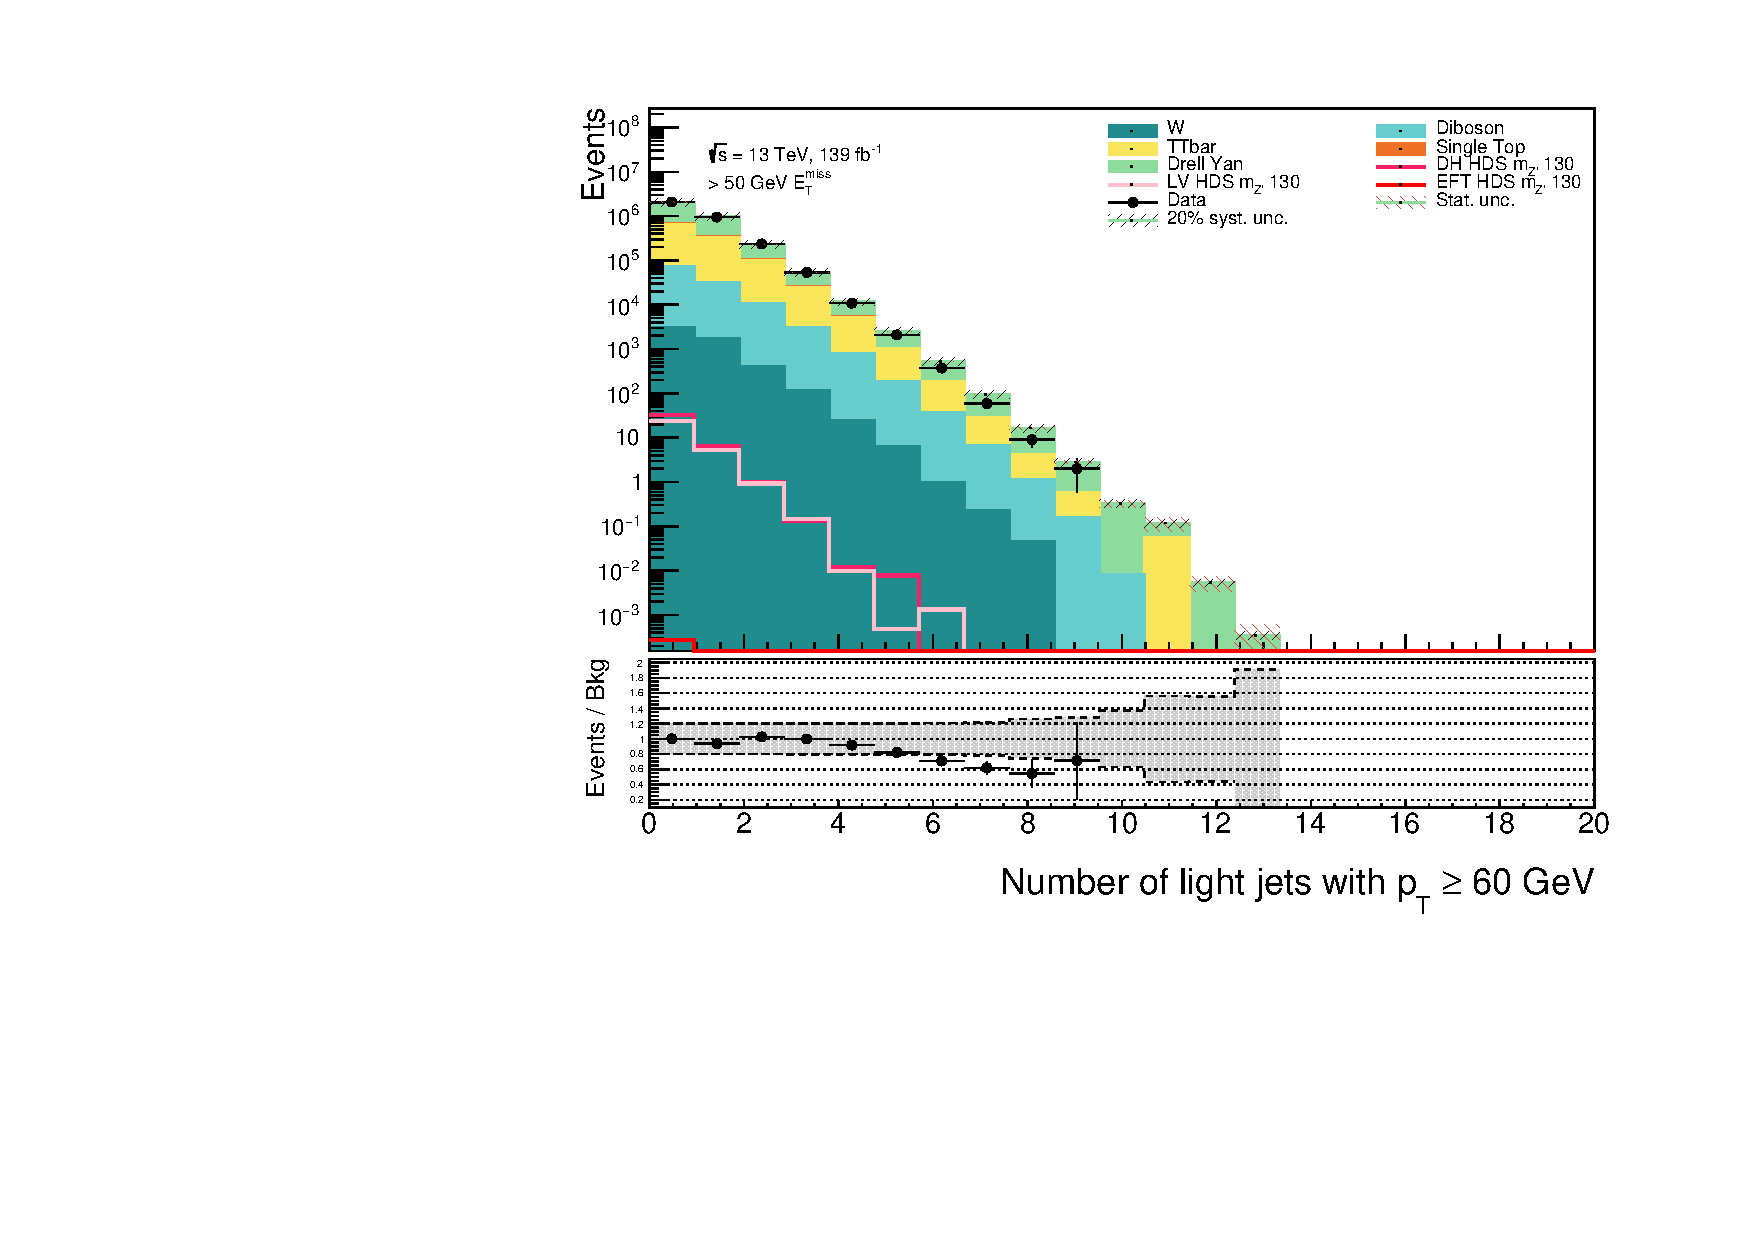
\includegraphics[width=\textwidth]{ljetsPt60.pdf}
%     \end{subfigure}
%     \caption{Data and MC agreement on number of light jets with different $p_T$ cuts in SR1.}
% \end{figure}

% \graphicspath{{../../Plots/Data_Analysis/JetSelection/100-150_MET-120_mll/}} 
% \begin{figure}[!ht]
%     \centering
%     \begin{subfigure}[b]{0.49\textwidth}
%         \centering
%         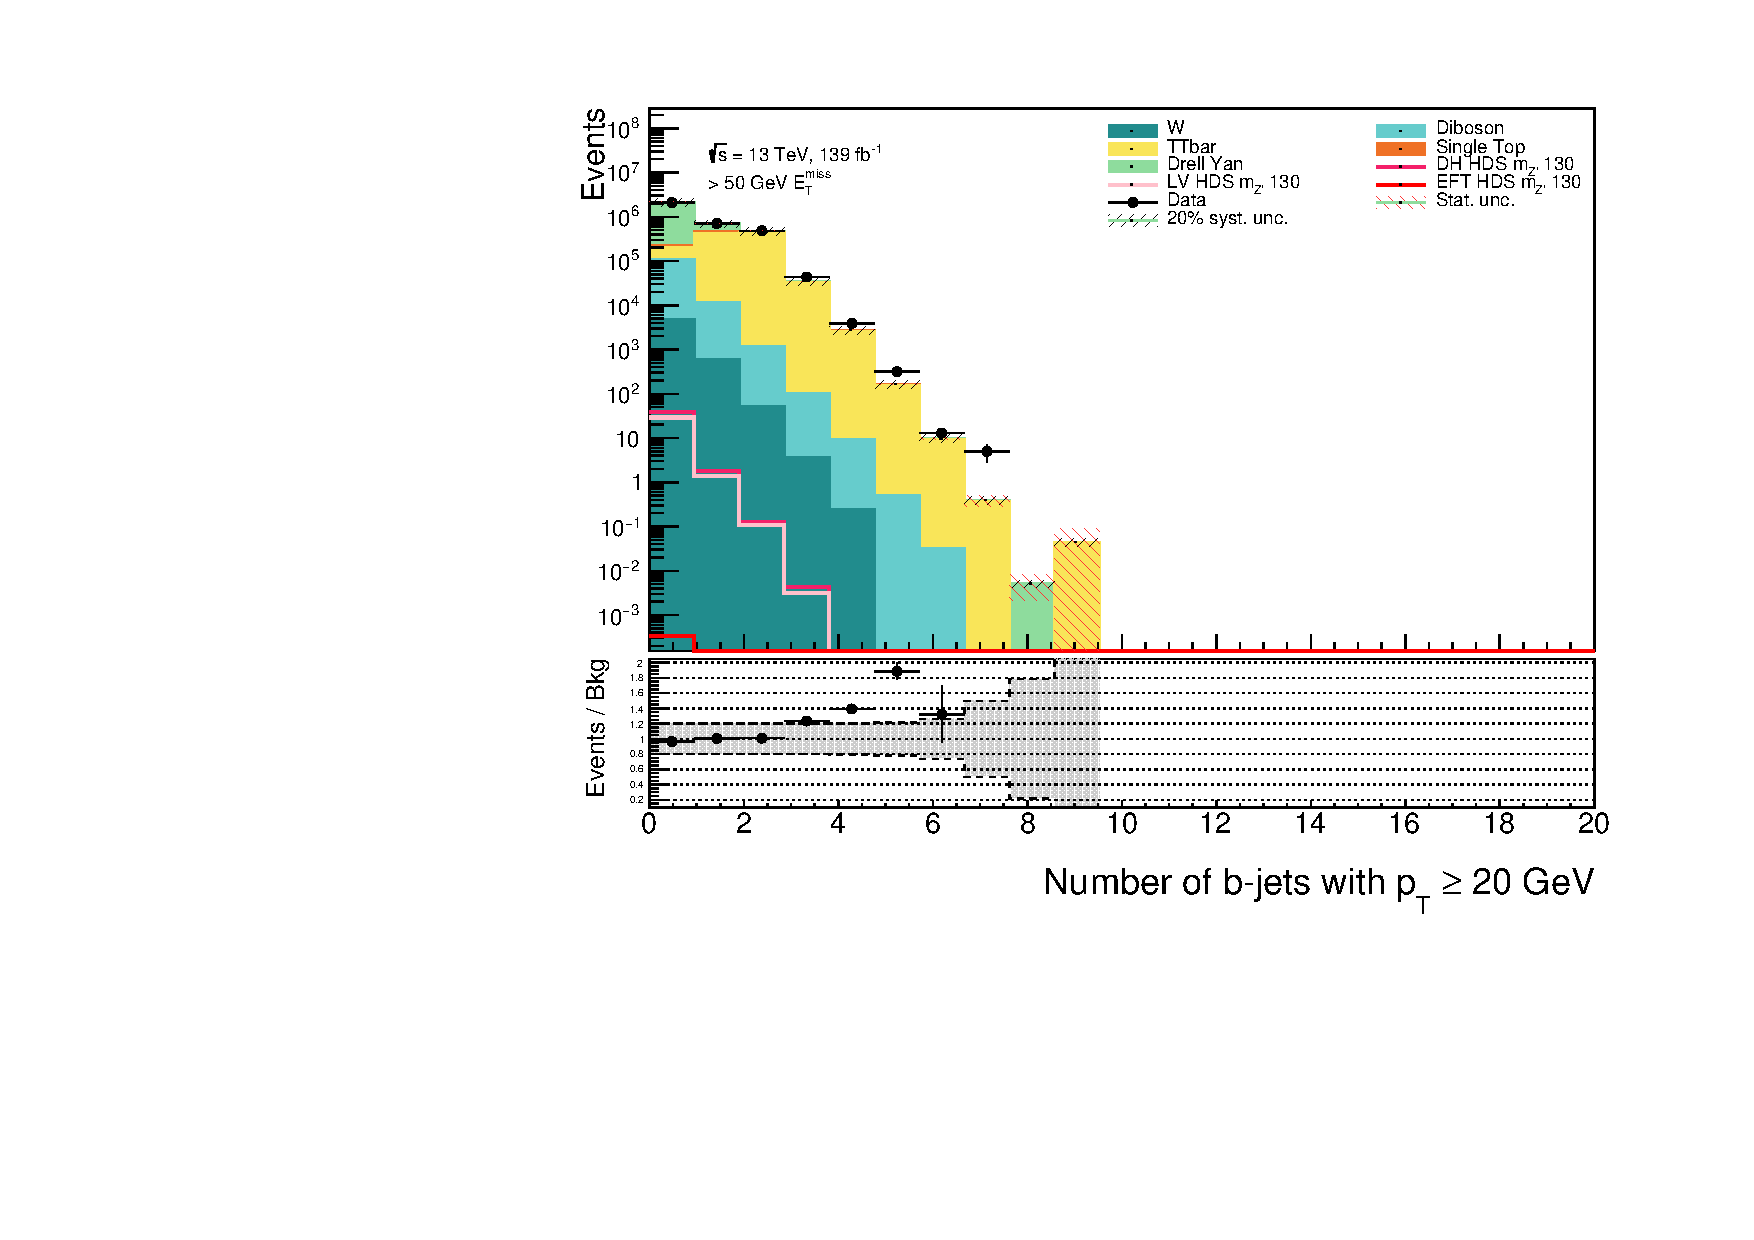
\includegraphics[width=\textwidth]{bjetsPt20.pdf}
%     \end{subfigure}
%     \hfill\begin{subfigure}[b]{0.49\textwidth}
%         \centering
%         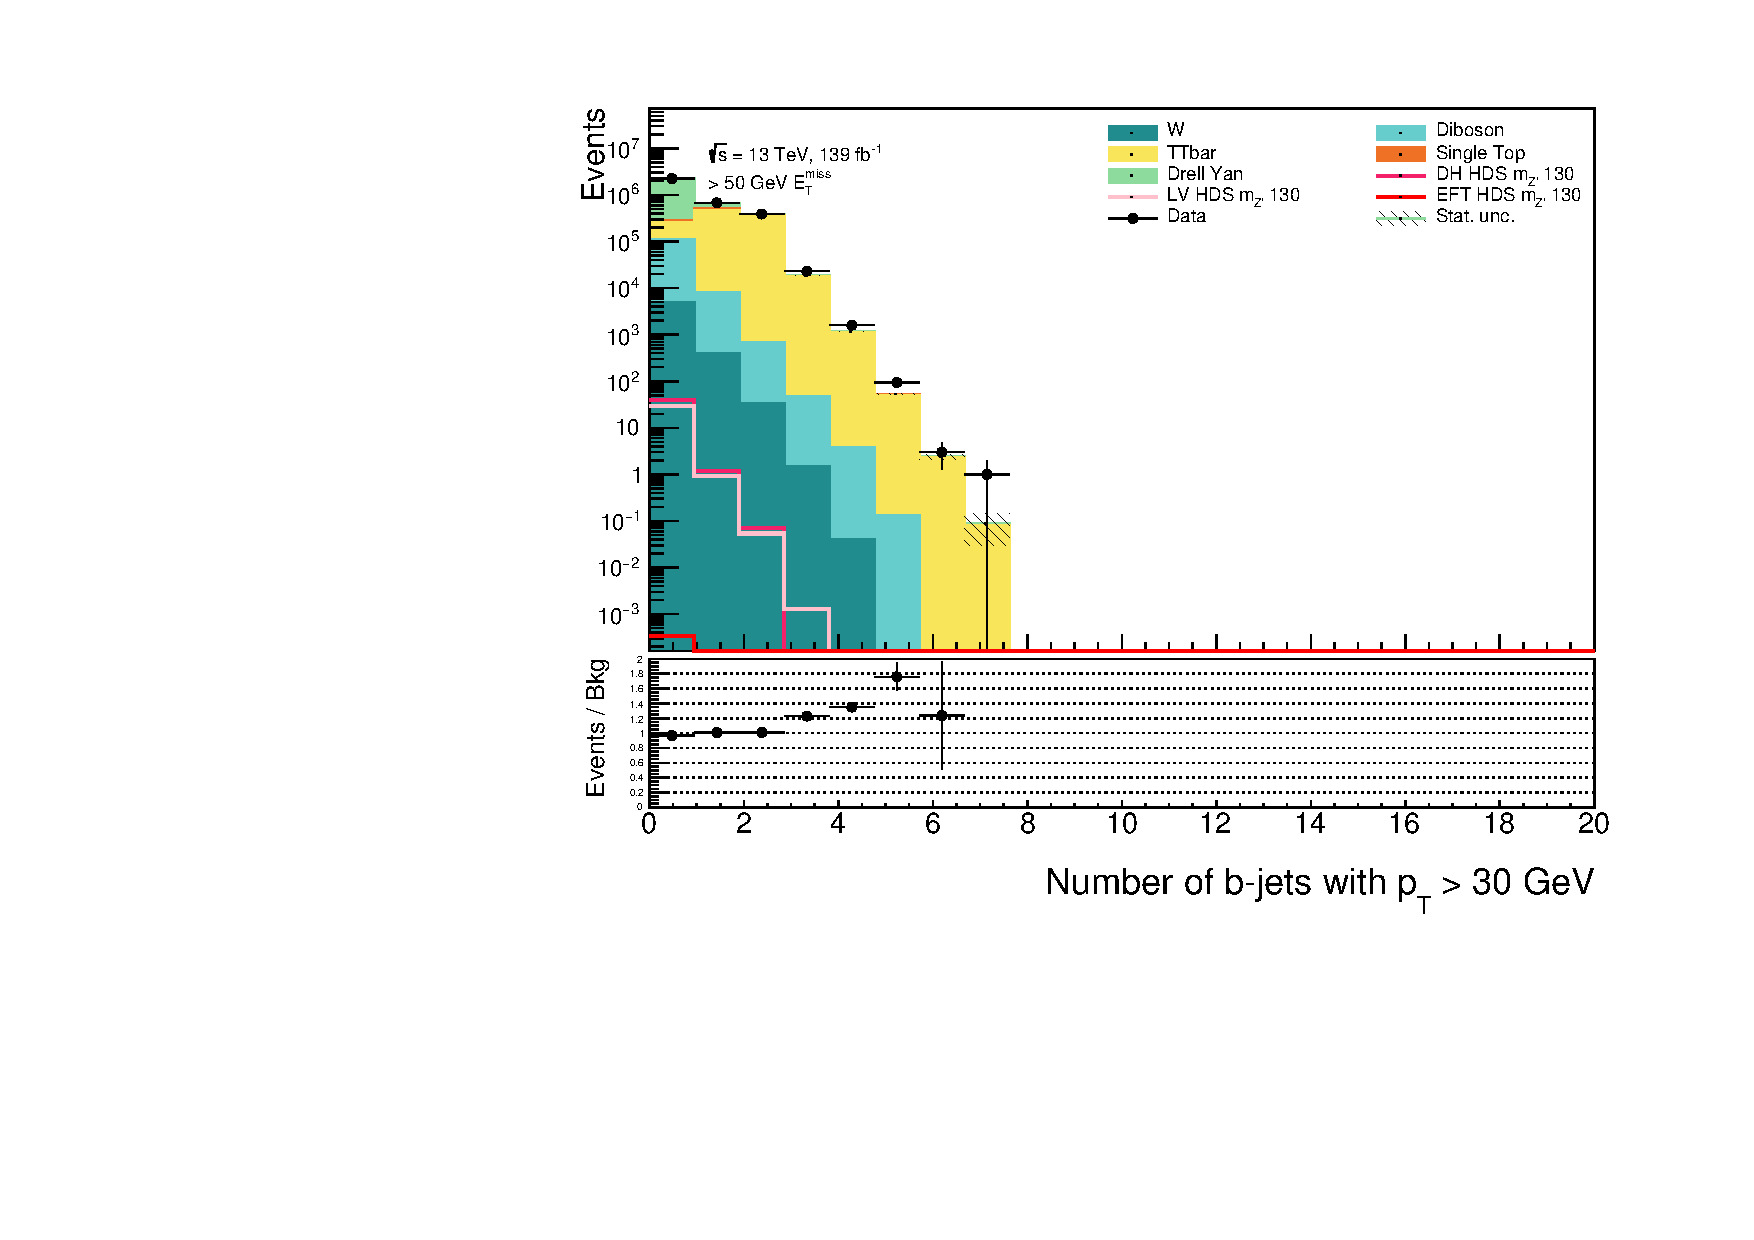
\includegraphics[width=\textwidth]{bjetsPt30.pdf}
%     \end{subfigure}
%     \hfill\begin{subfigure}[b]{0.49\textwidth}
%         \centering
%         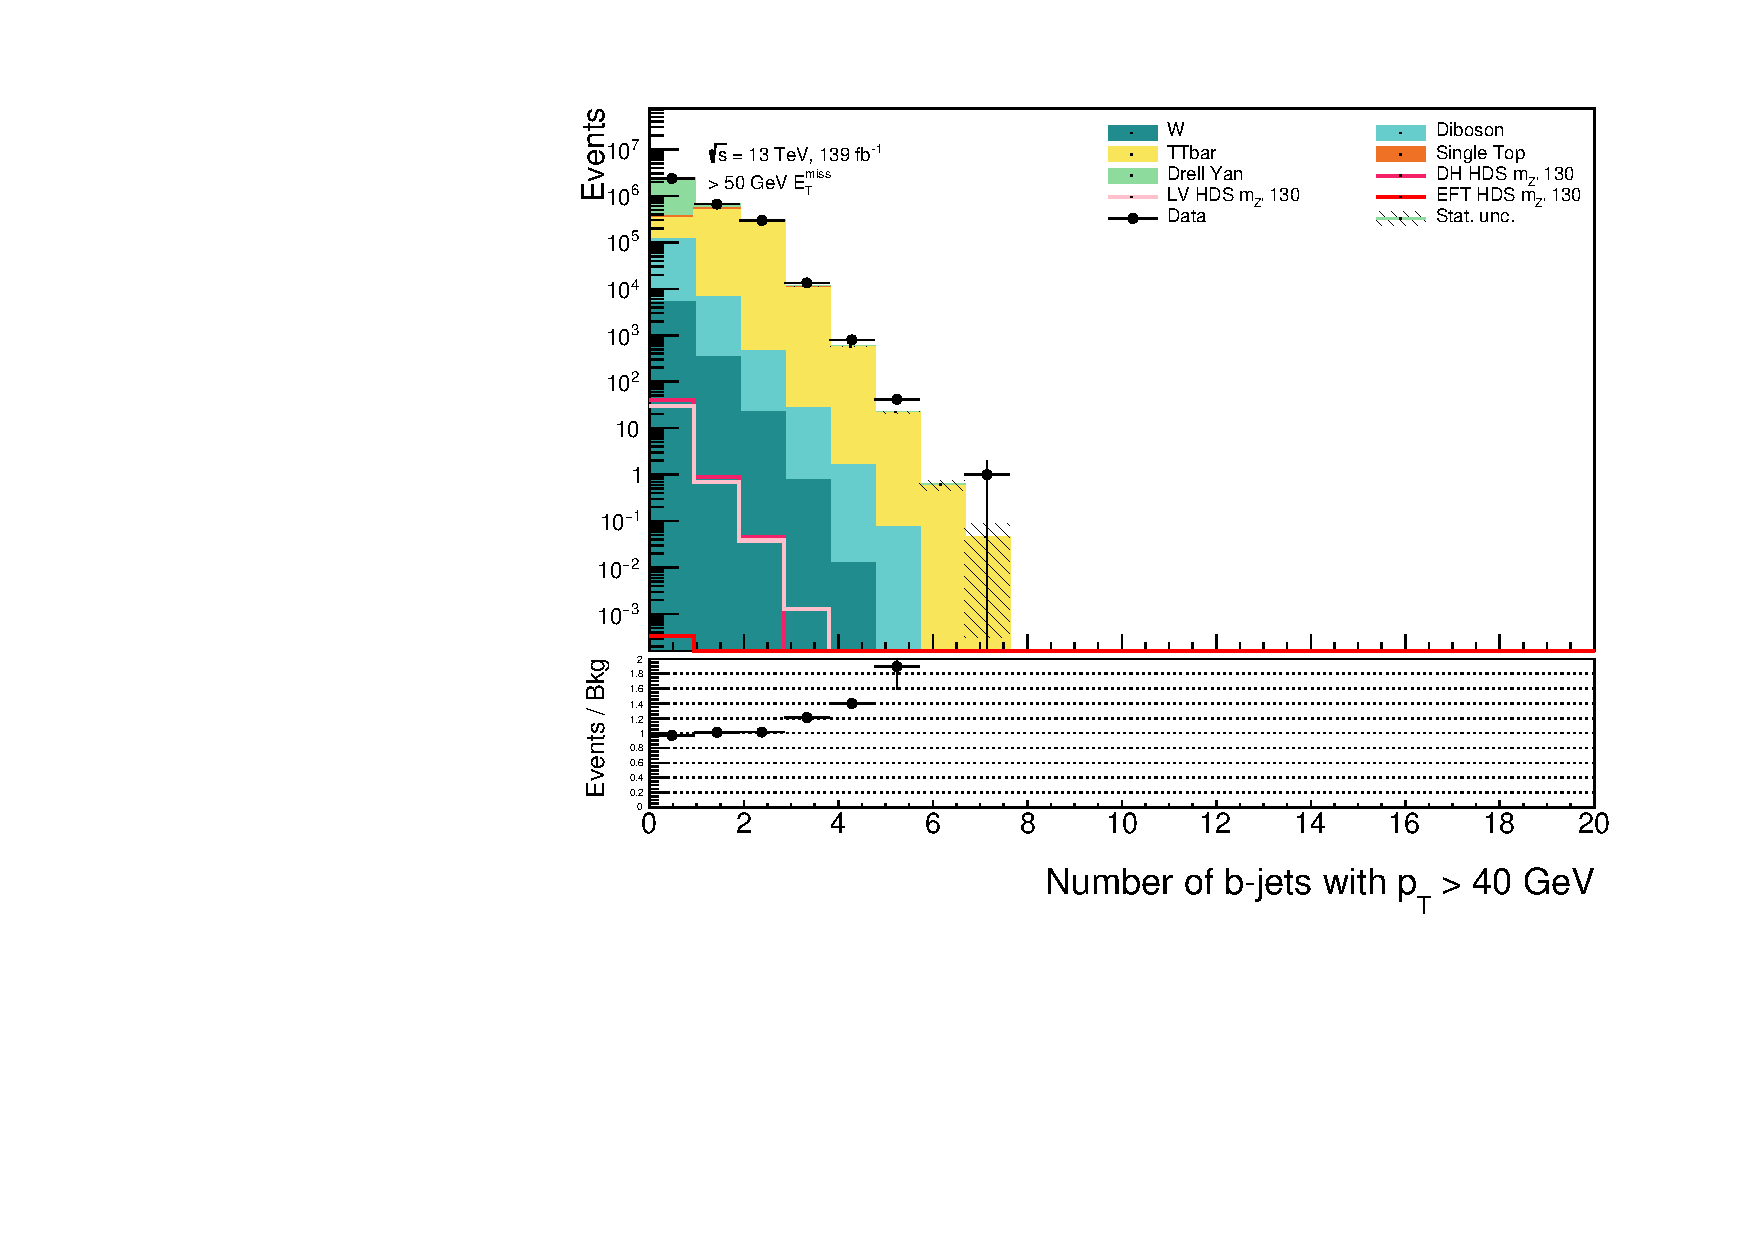
\includegraphics[width=\textwidth]{bjetsPt40.pdf}
%     \end{subfigure}
%     \hfill\begin{subfigure}[b]{0.49\textwidth}
%         \centering
%         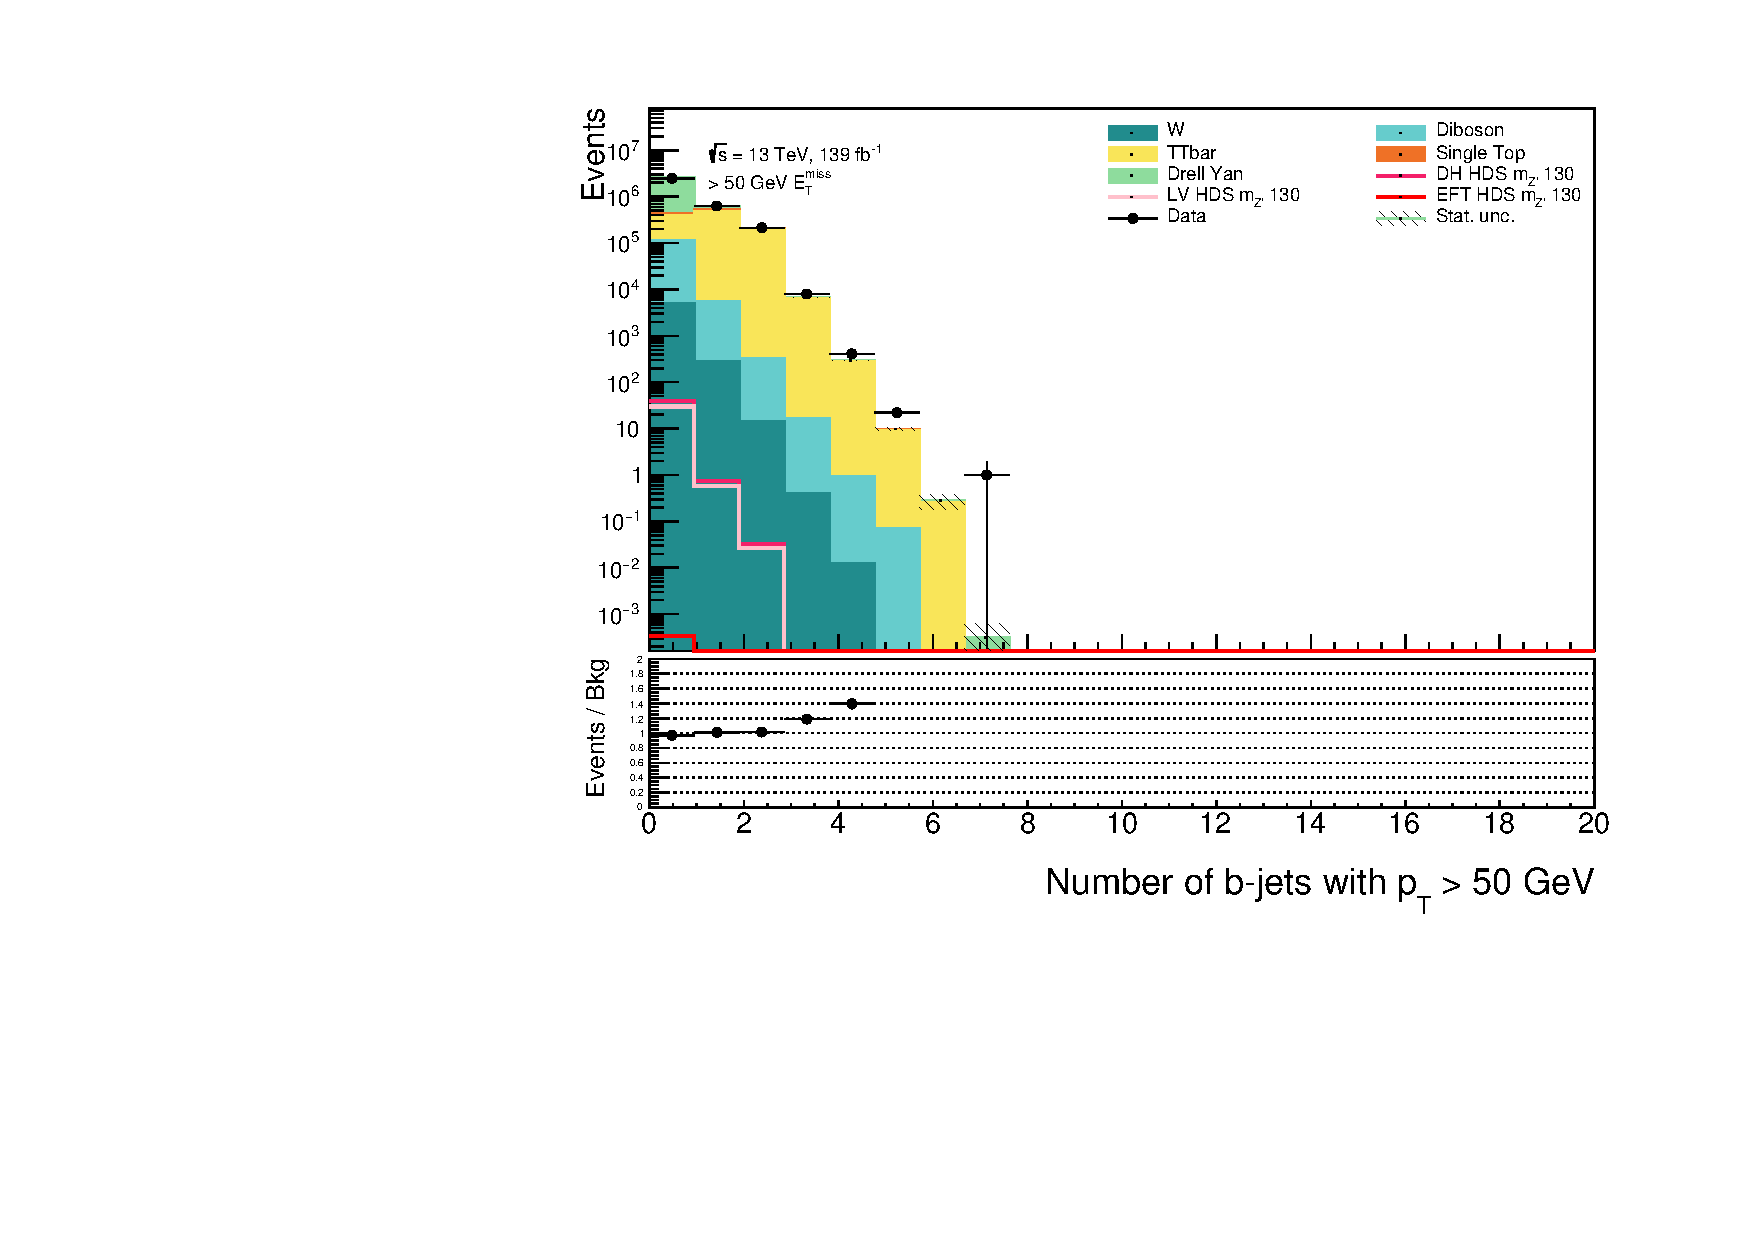
\includegraphics[width=\textwidth]{bjetsPt50.pdf}
%     \end{subfigure}
%     \hfill\begin{subfigure}[b]{0.49\textwidth}
%         \centering
%         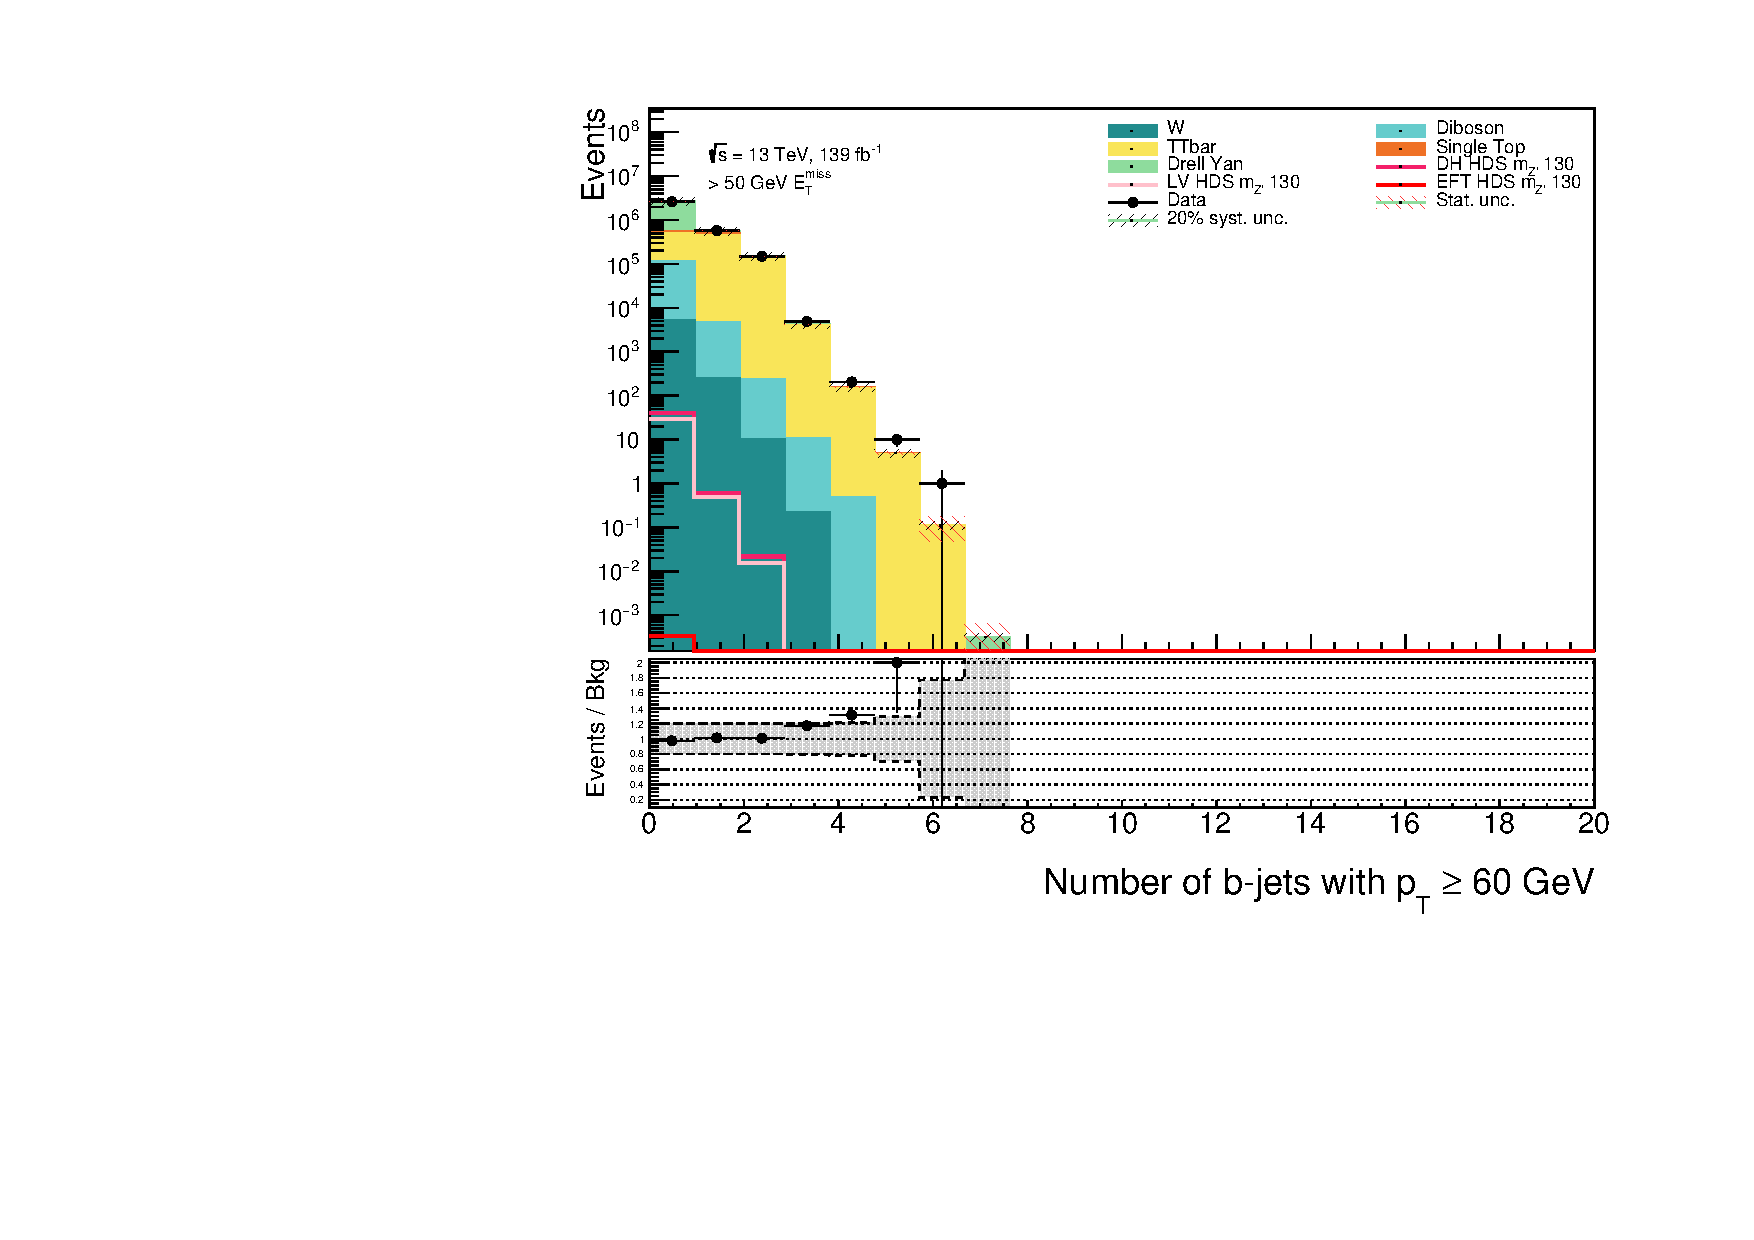
\includegraphics[width=\textwidth]{bjetsPt60.pdf}
%     \end{subfigure}
%     \caption{Data and MC agreement on number of b- jets with different $p_T$ cuts in SR2.}
% \end{figure}

% \begin{figure}[!ht]
%     \centering
%     \begin{subfigure}[b]{0.49\textwidth}
%         \centering
%         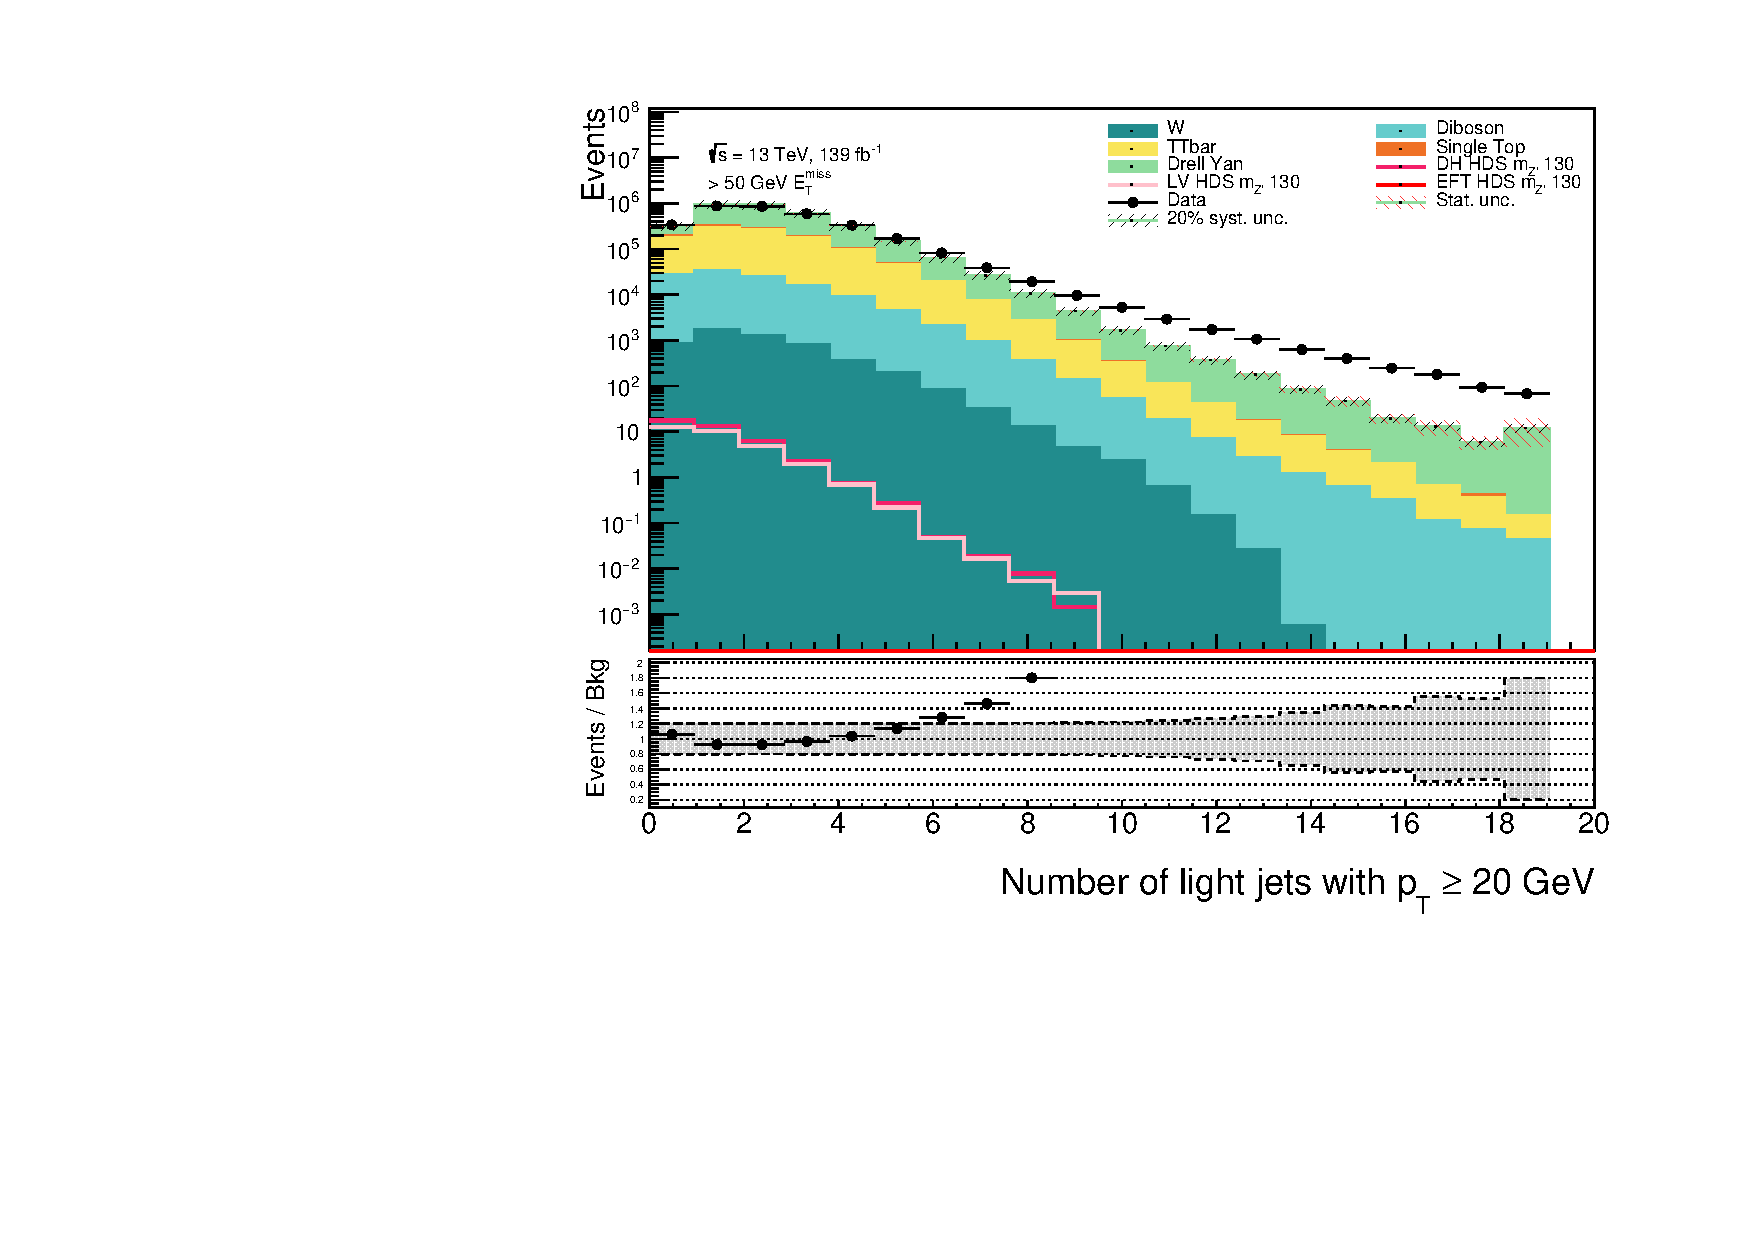
\includegraphics[width=\textwidth]{ljetsPt20.pdf}
%     \end{subfigure}
%     \hfill\begin{subfigure}[b]{0.49\textwidth}
%         \centering
%         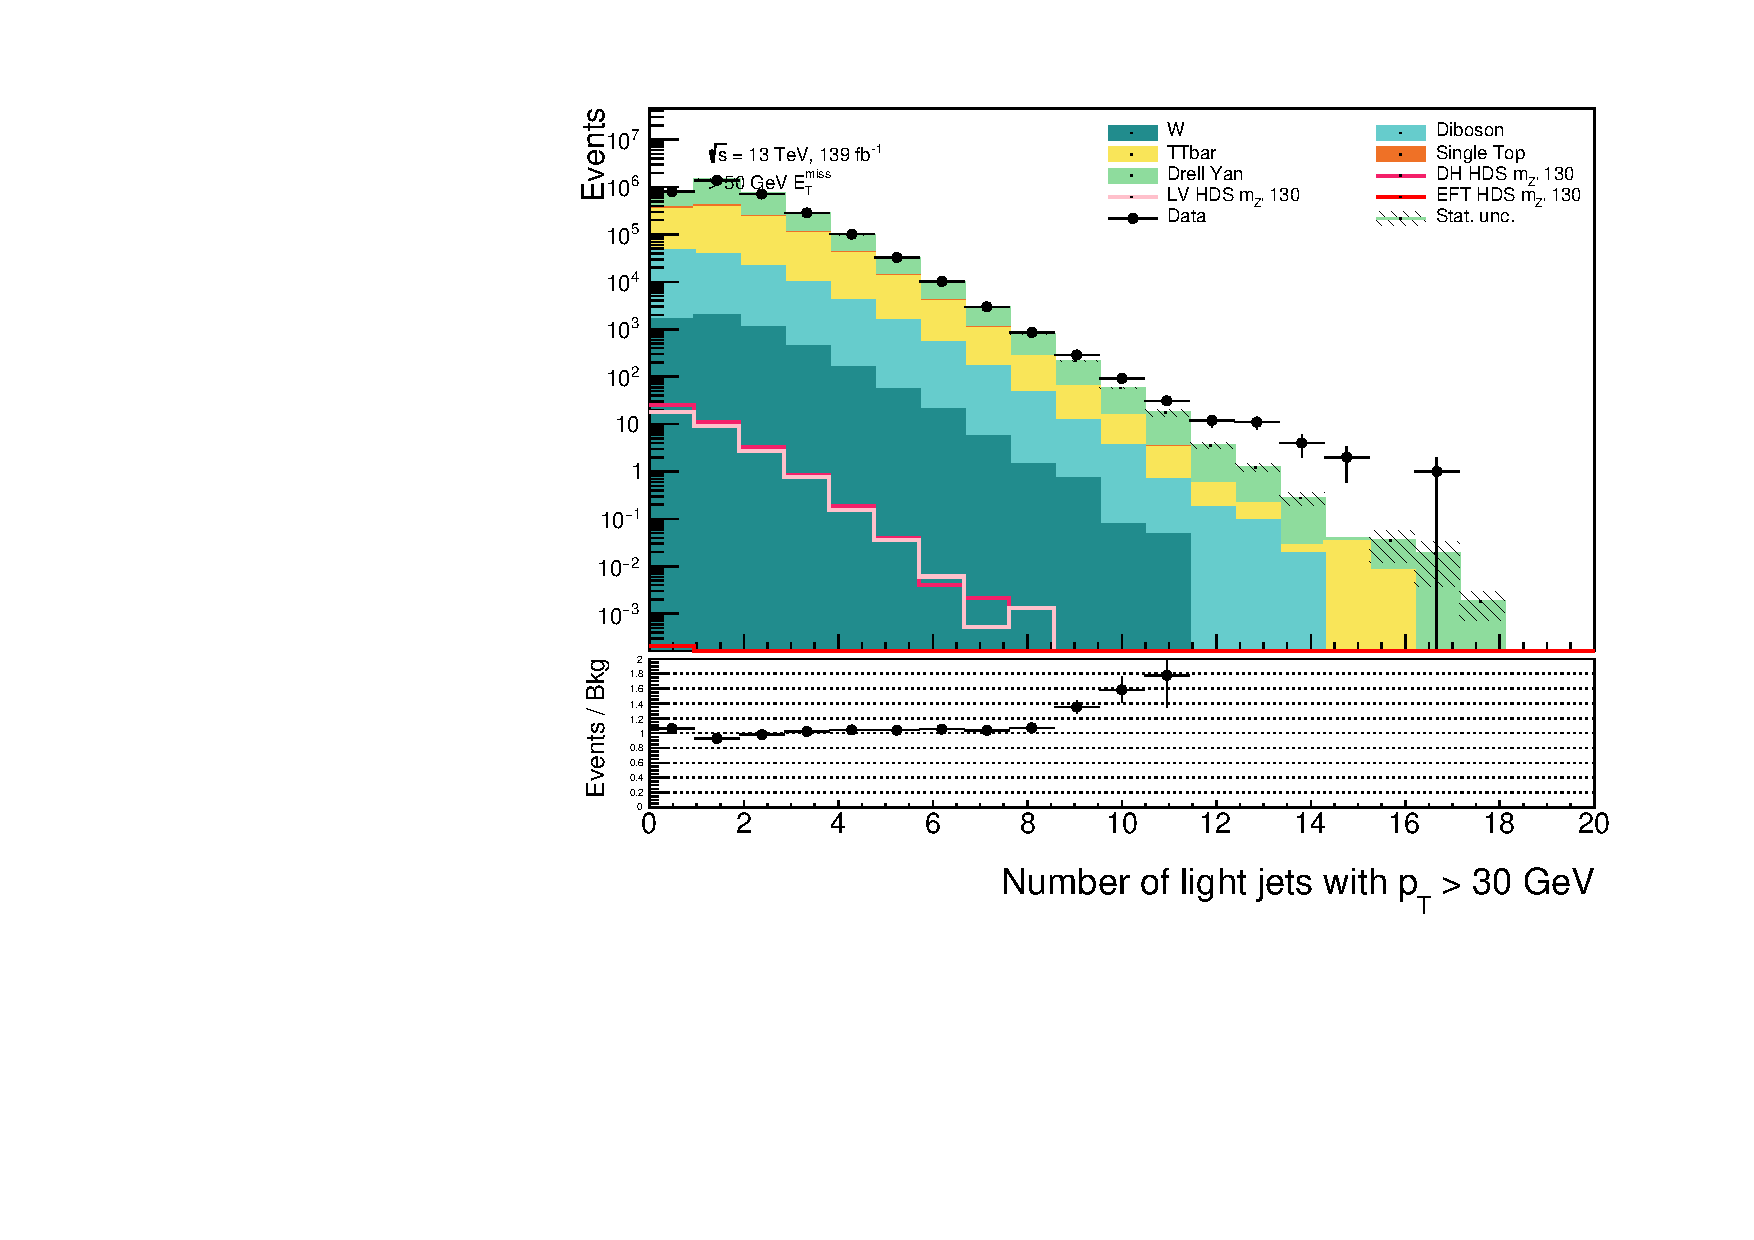
\includegraphics[width=\textwidth]{ljetsPt30.pdf}
%     \end{subfigure}
%     \hfill\begin{subfigure}[b]{0.49\textwidth}
%         \centering
%         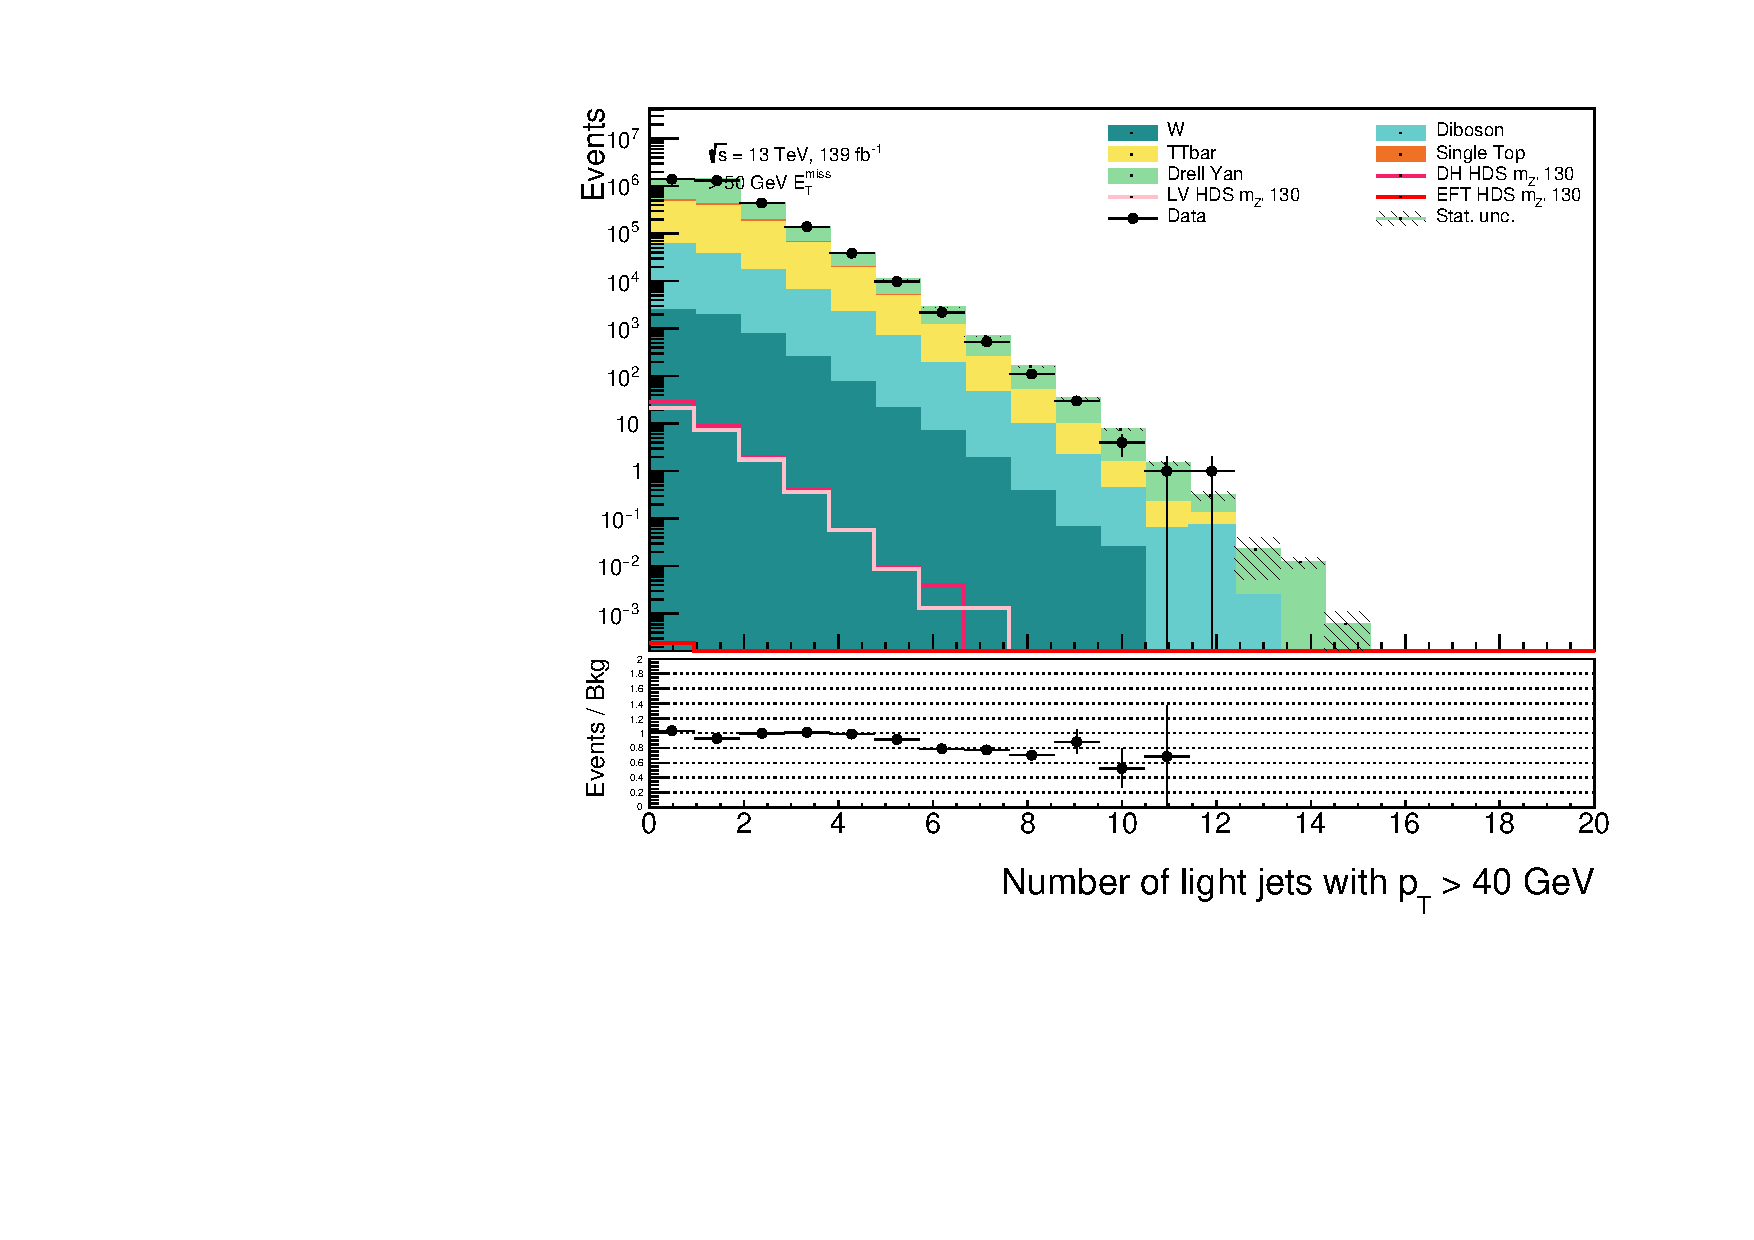
\includegraphics[width=\textwidth]{ljetsPt40.pdf}
%     \end{subfigure}
%     \hfill\begin{subfigure}[b]{0.49\textwidth}
%         \centering
%         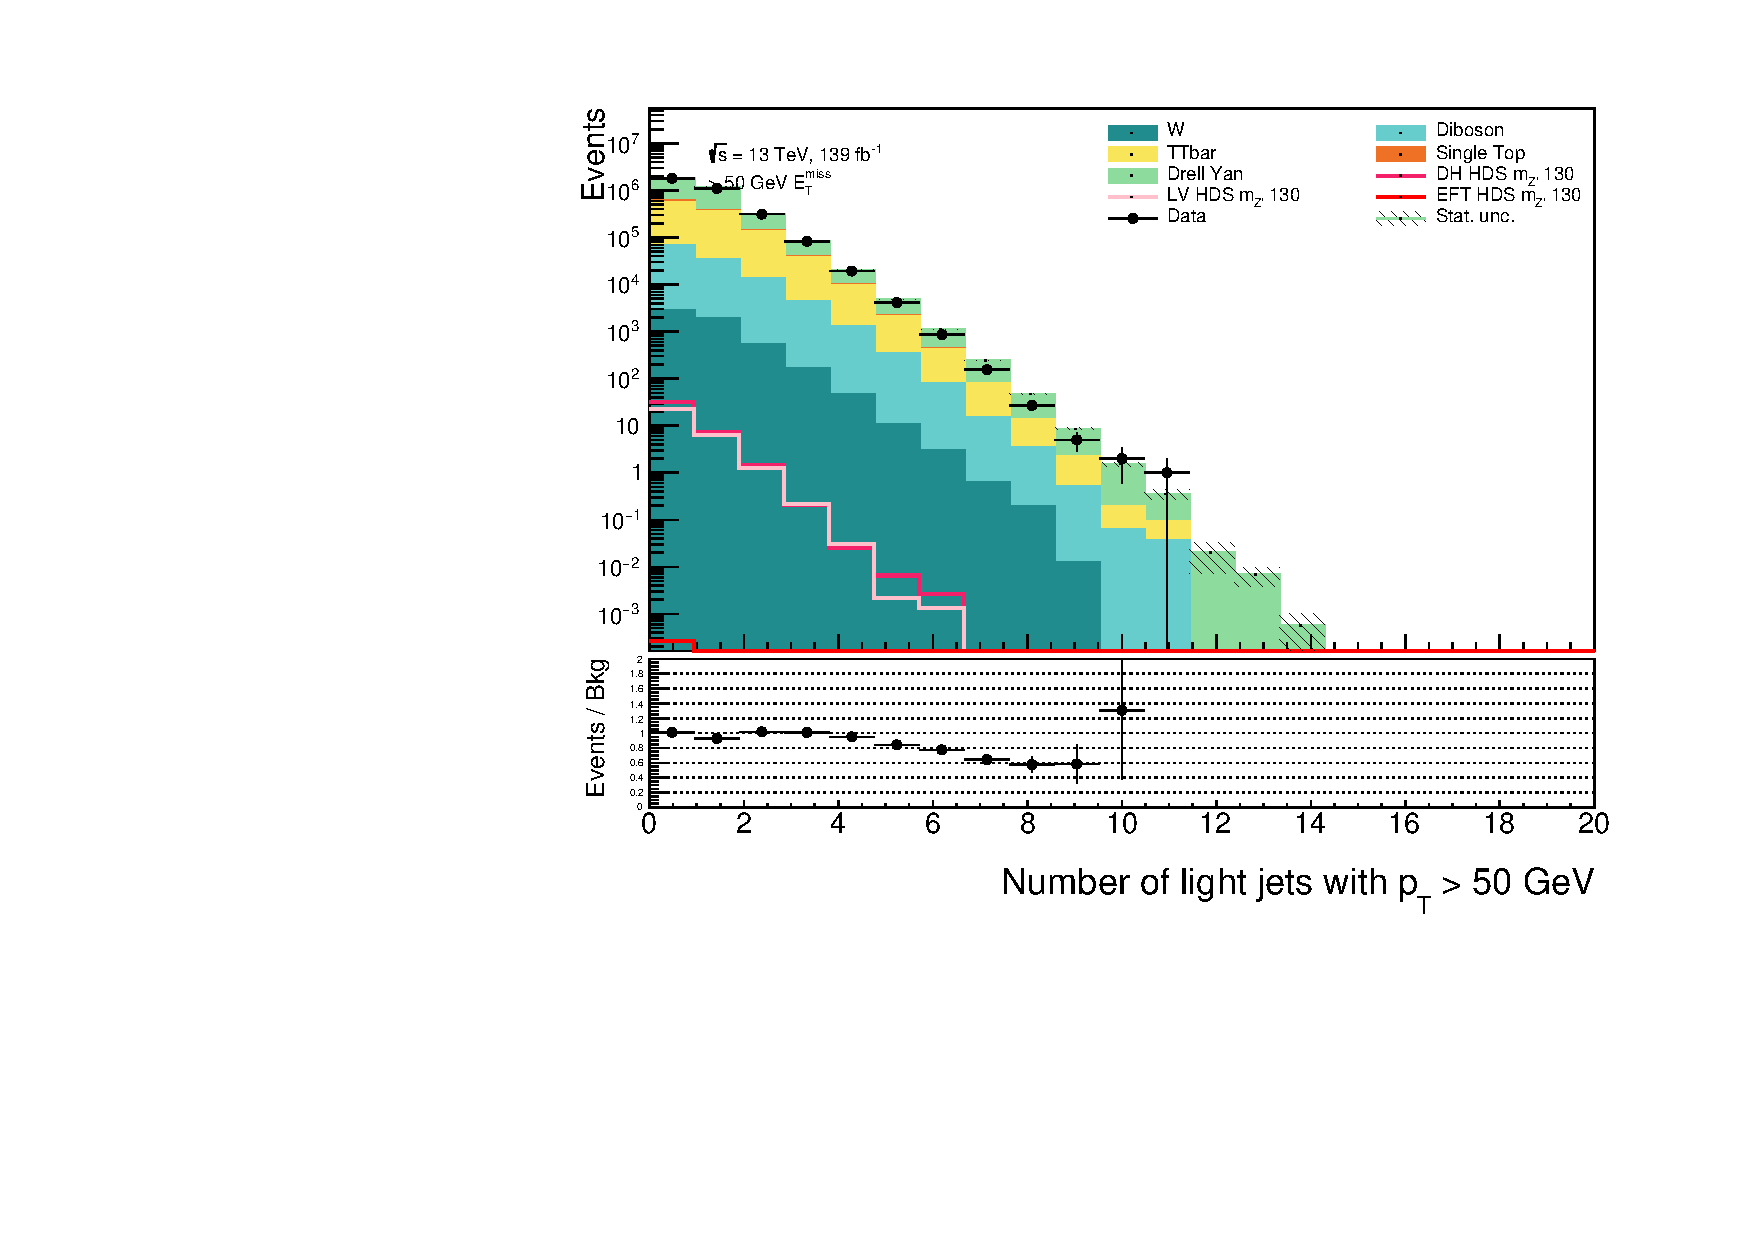
\includegraphics[width=\textwidth]{ljetsPt50.pdf}
%     \end{subfigure}
%     \hfill\begin{subfigure}[b]{0.49\textwidth}
%         \centering
%         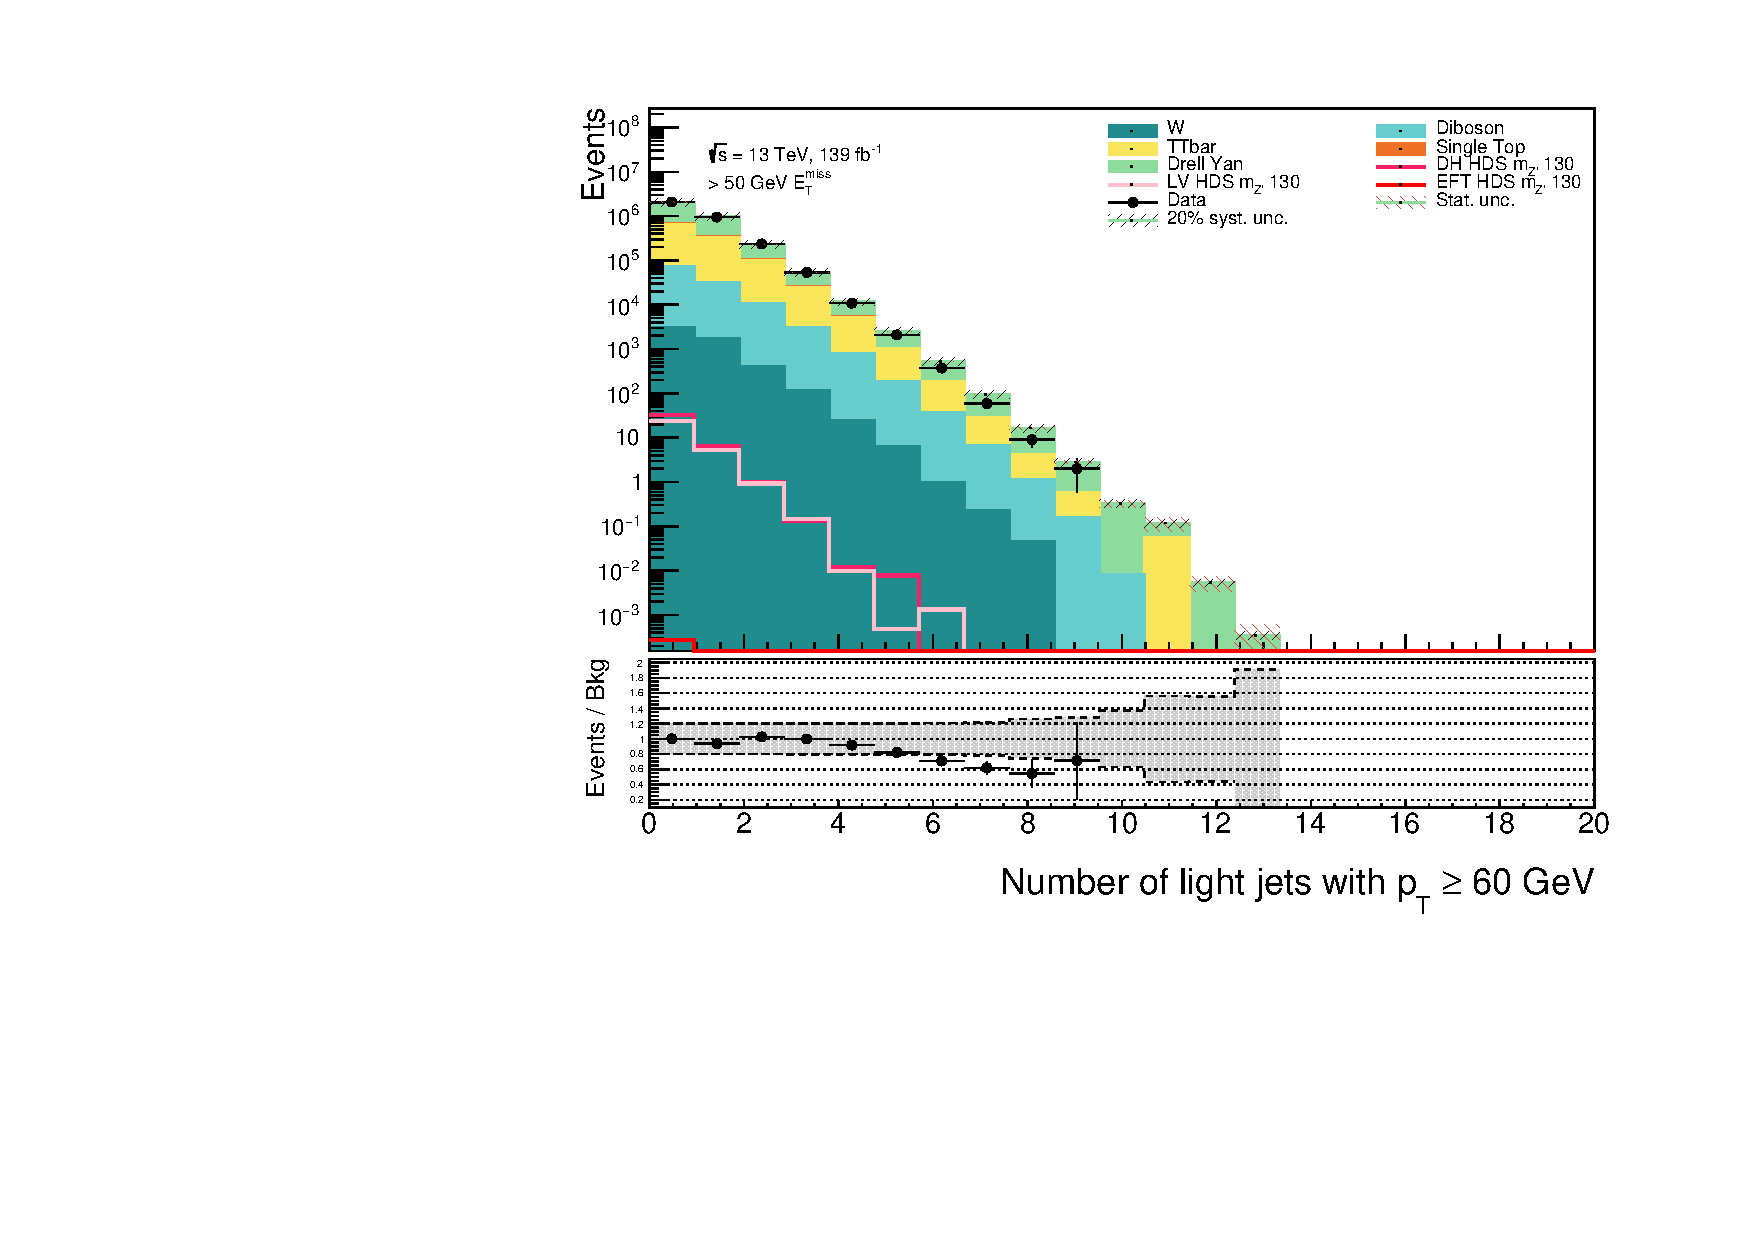
\includegraphics[width=\textwidth]{ljetsPt60.pdf}
%     \end{subfigure}
%     \caption{Data and MC agreement on number of light jets with different $p_T$ cuts in SR2.}
% \end{figure}

% \graphicspath{{../../Plots/Data_Analysis/JetSelection/150_MET-120_mll/}} 
% \begin{figure}[!ht]
%     \centering
%     \begin{subfigure}[b]{0.49\textwidth}
%         \centering
%         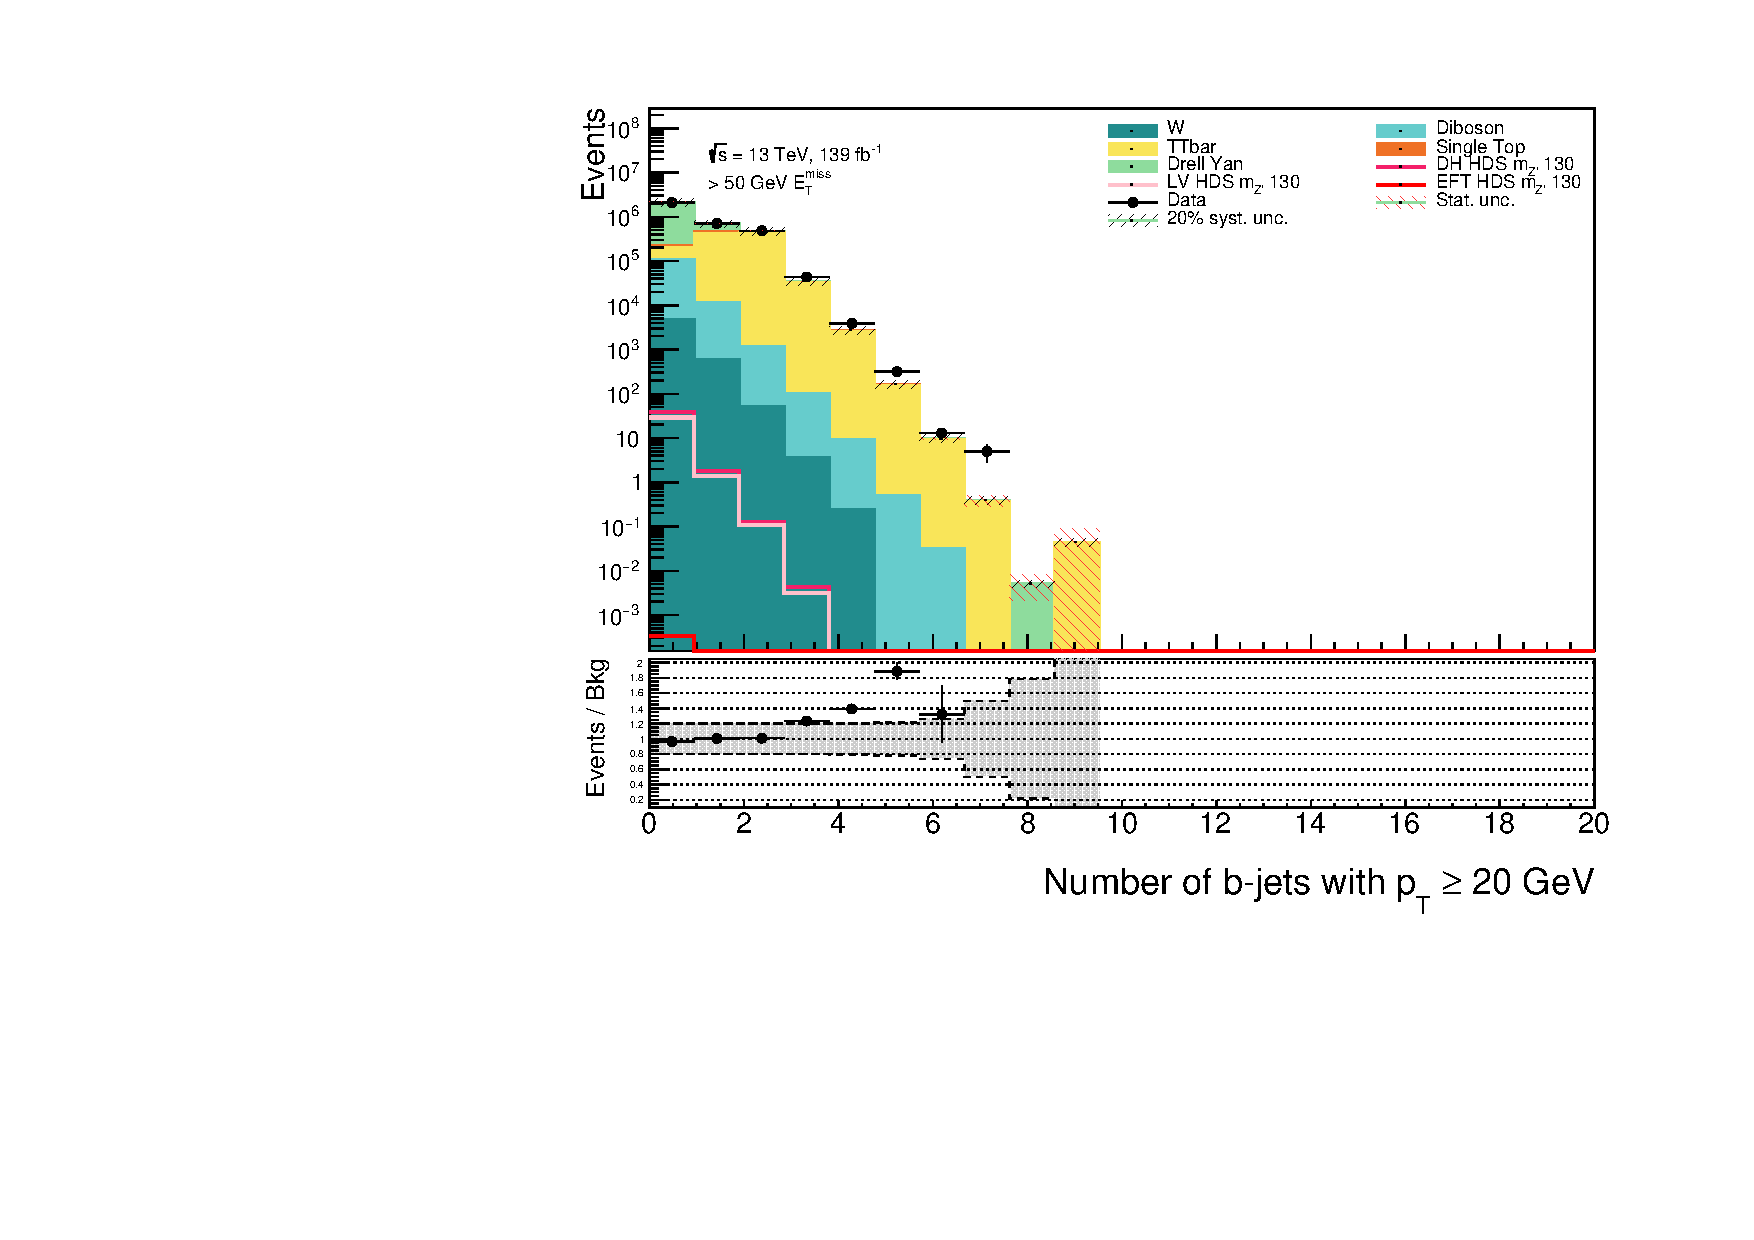
\includegraphics[width=\textwidth]{bjetsPt20.pdf}
%     \end{subfigure}
%     \hfill\begin{subfigure}[b]{0.49\textwidth}
%         \centering
%         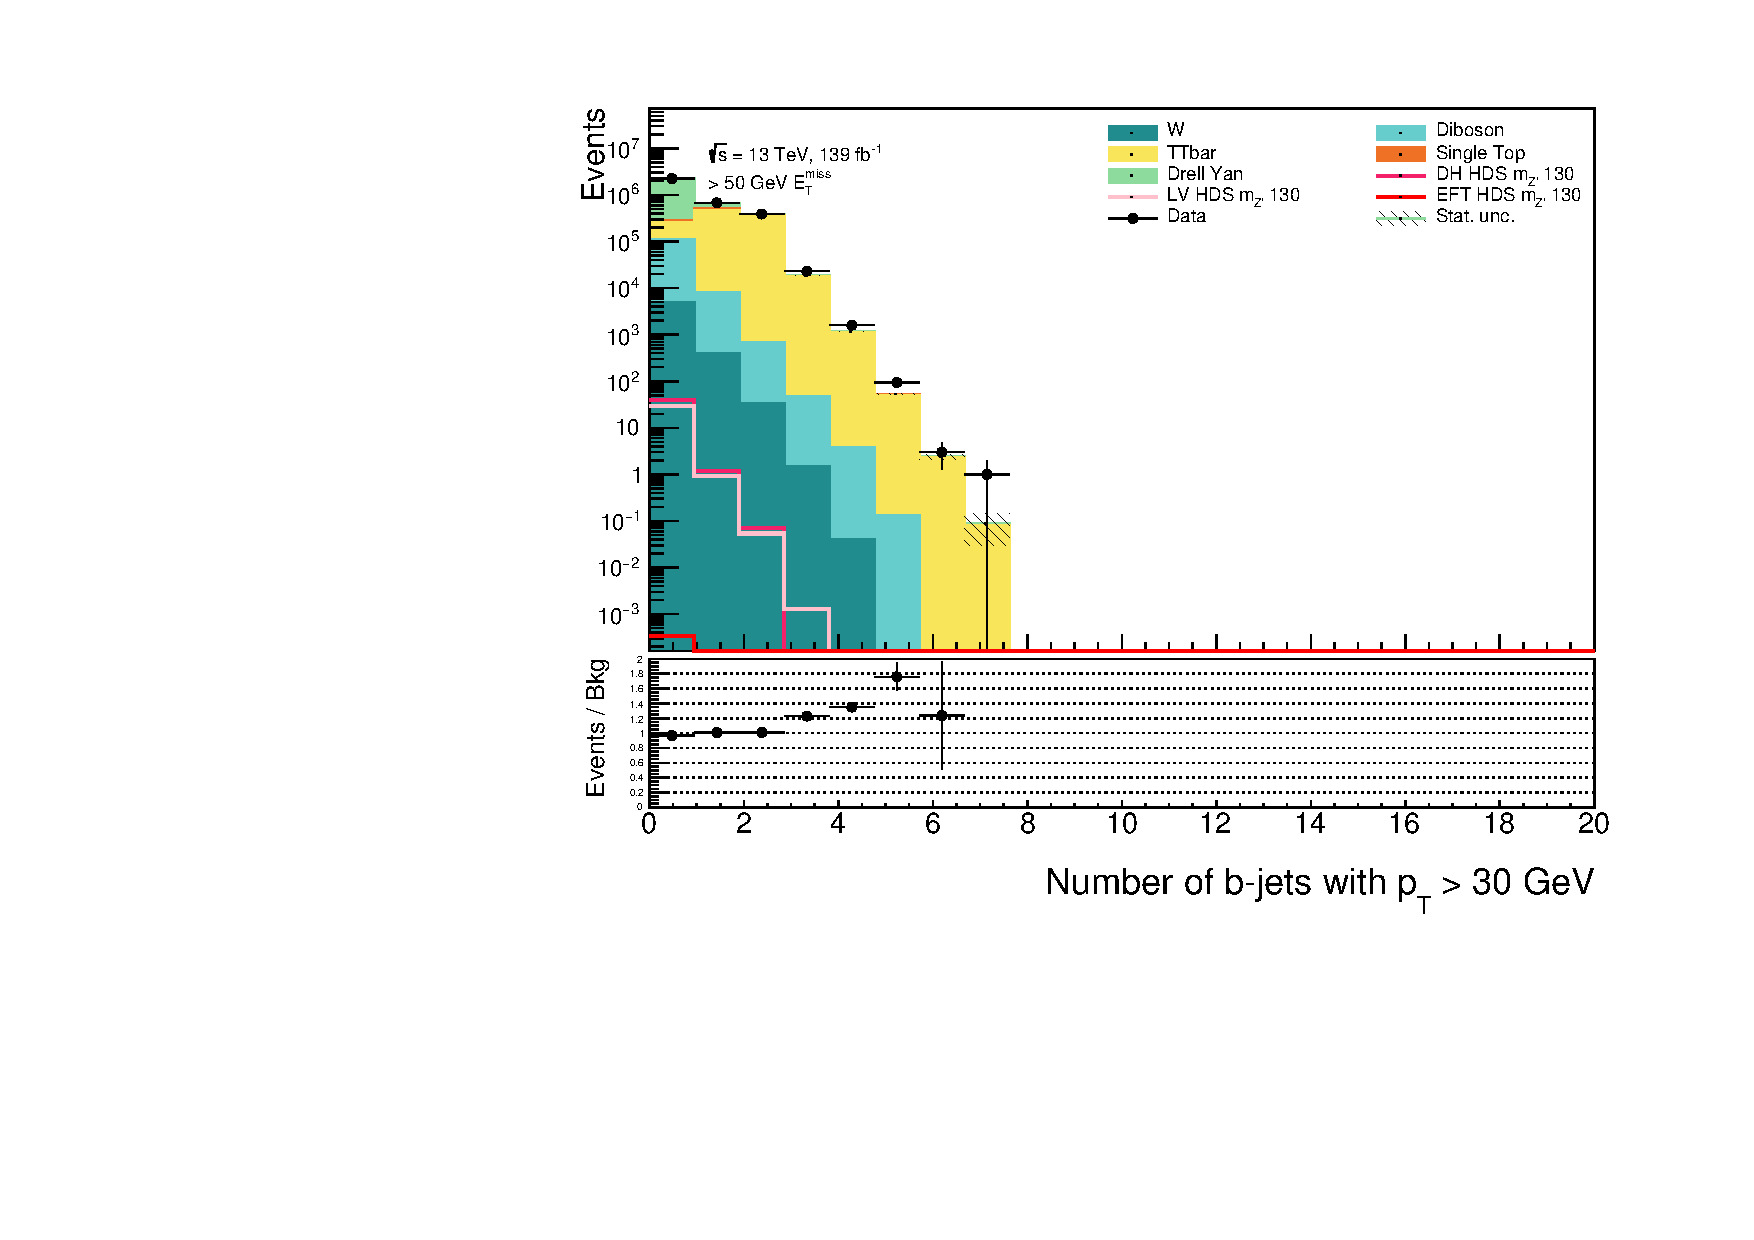
\includegraphics[width=\textwidth]{bjetsPt30.pdf}
%     \end{subfigure}
%     \hfill\begin{subfigure}[b]{0.49\textwidth}
%         \centering
%         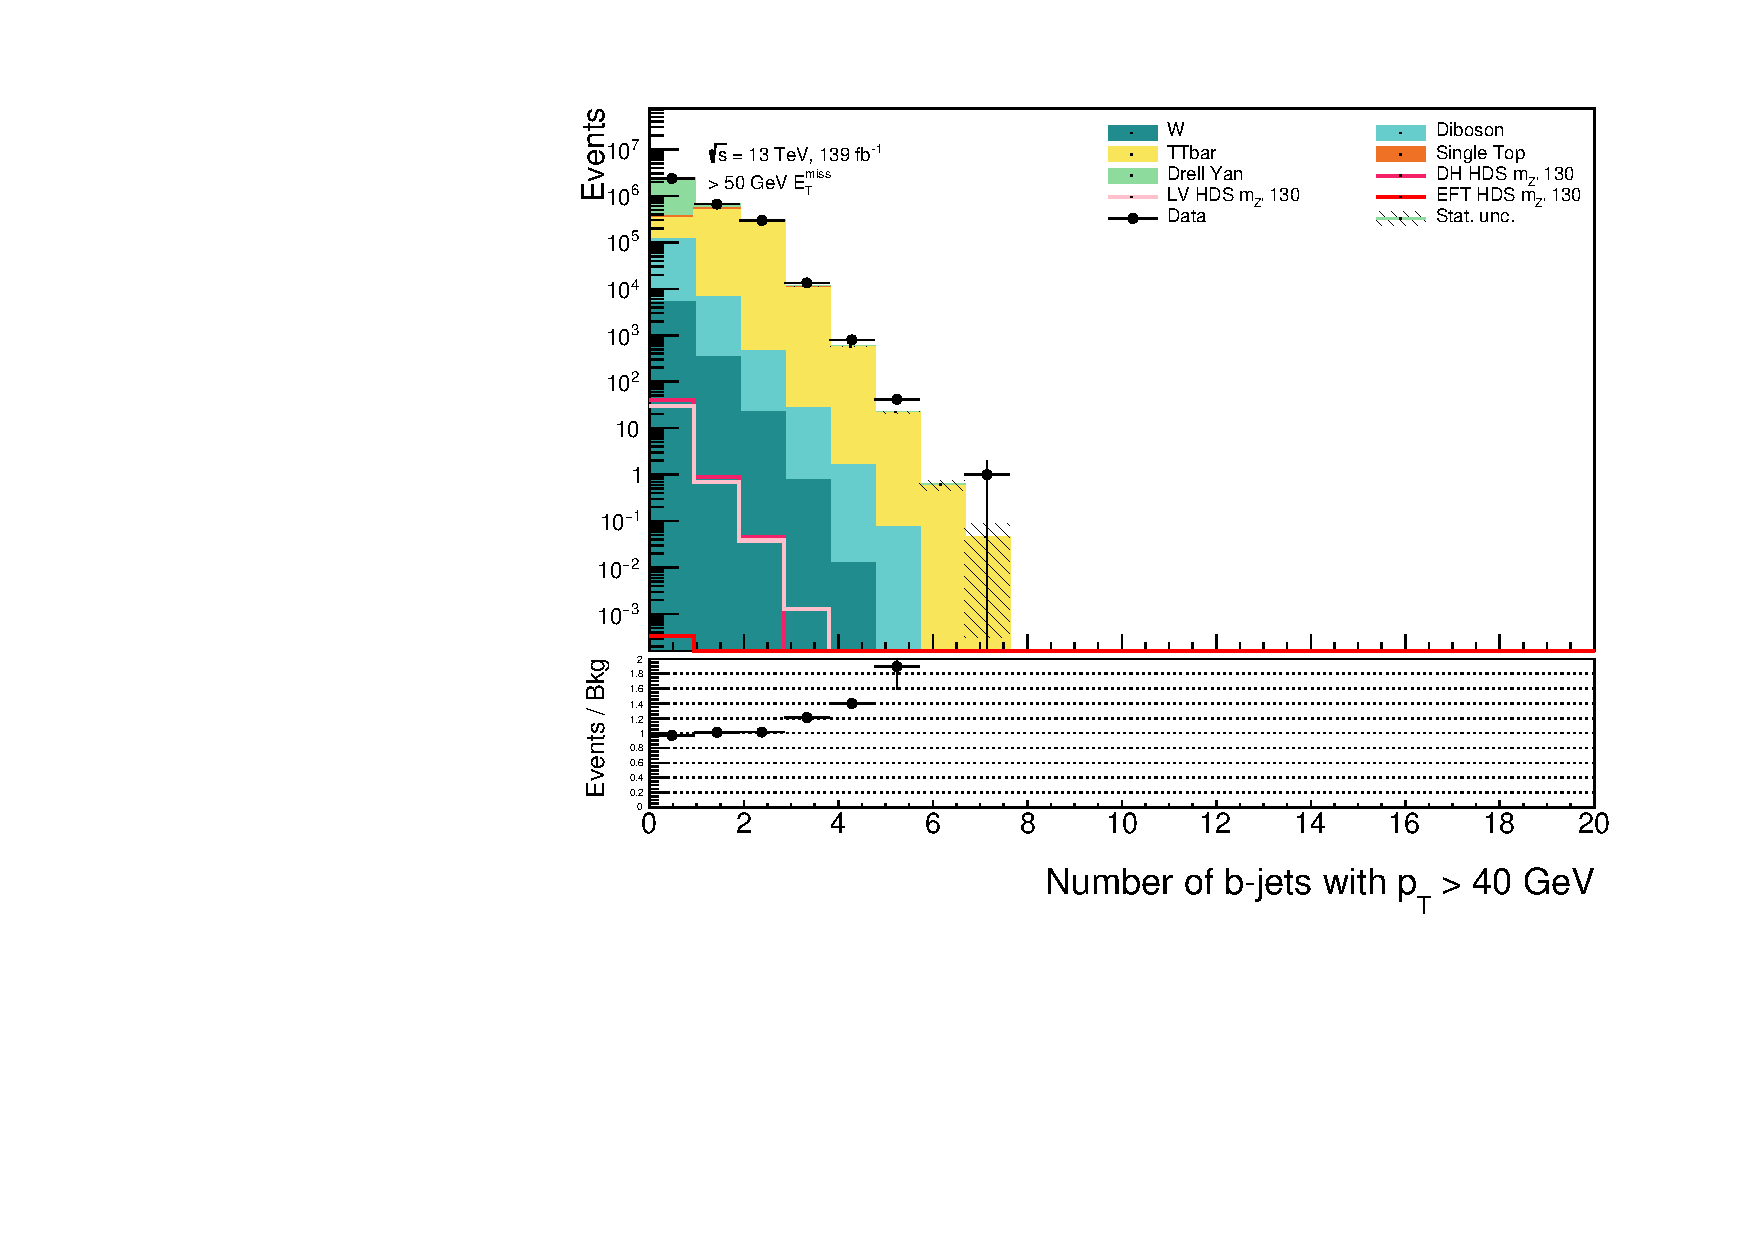
\includegraphics[width=\textwidth]{bjetsPt40.pdf}
%     \end{subfigure}
%     \hfill\begin{subfigure}[b]{0.49\textwidth}
%         \centering
%         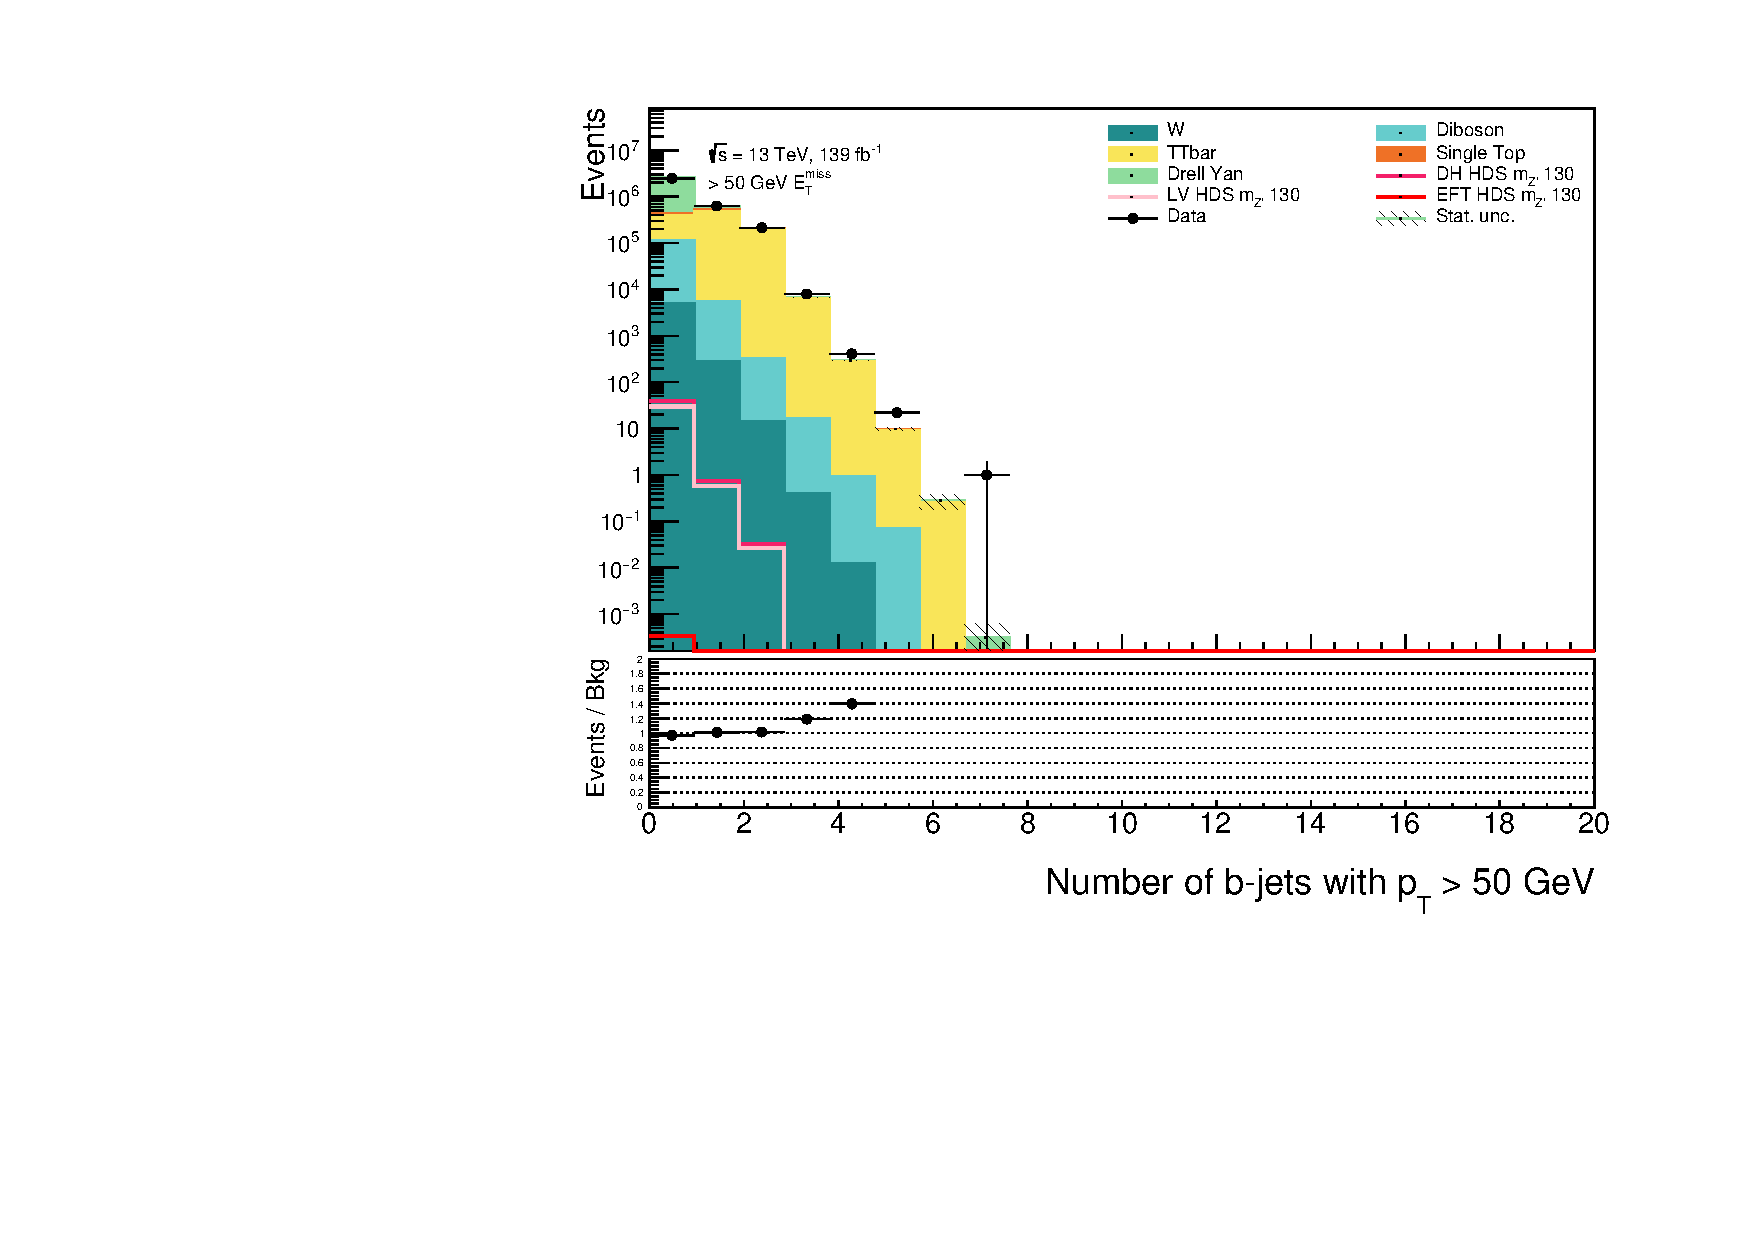
\includegraphics[width=\textwidth]{bjetsPt50.pdf}
%     \end{subfigure}
%     \hfill\begin{subfigure}[b]{0.49\textwidth}
%         \centering
%         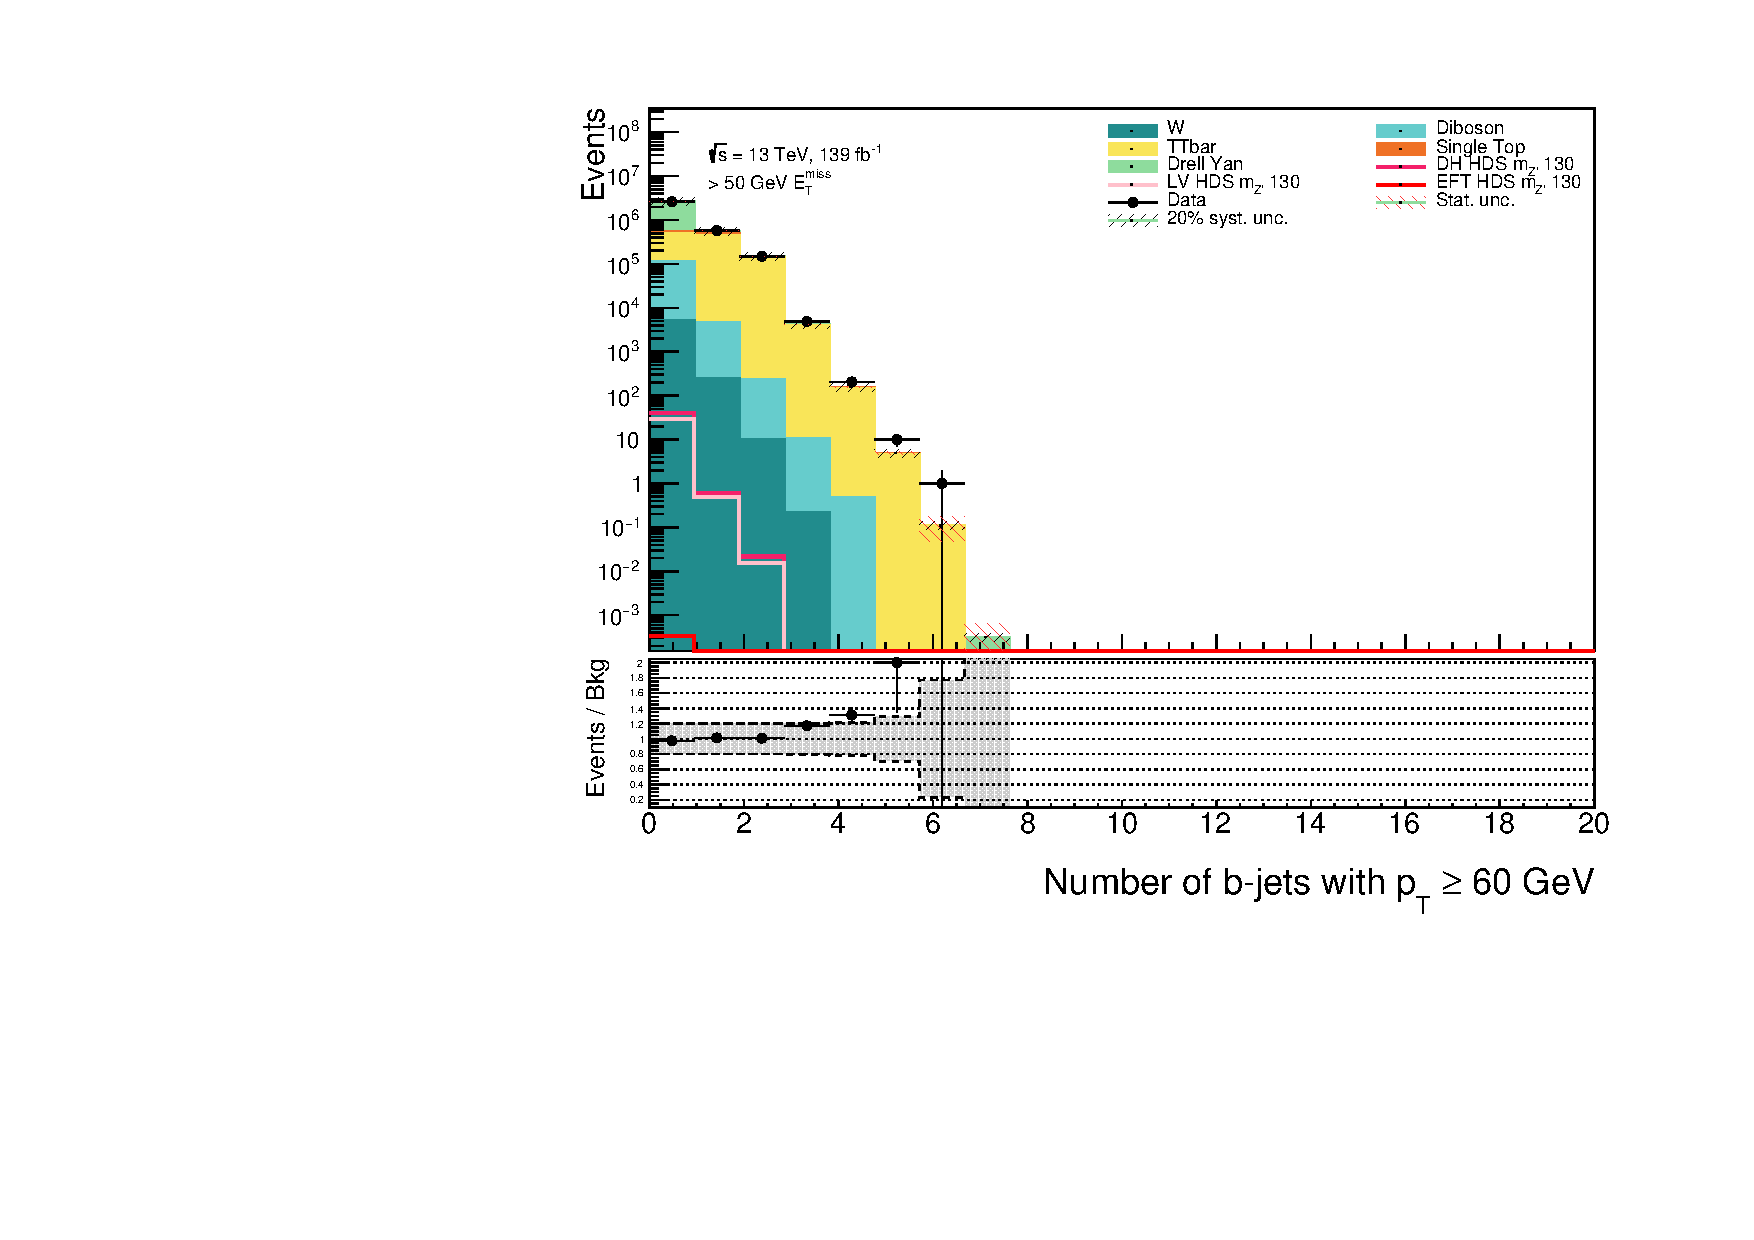
\includegraphics[width=\textwidth]{bjetsPt60.pdf}
%     \end{subfigure}
%     \caption{Data and MC agreement on number of b- jets with different $p_T$ cuts in SR3.}
% \end{figure}

% \begin{figure}[!ht]
%     \centering
%     \begin{subfigure}[b]{0.49\textwidth}
%         \centering
%         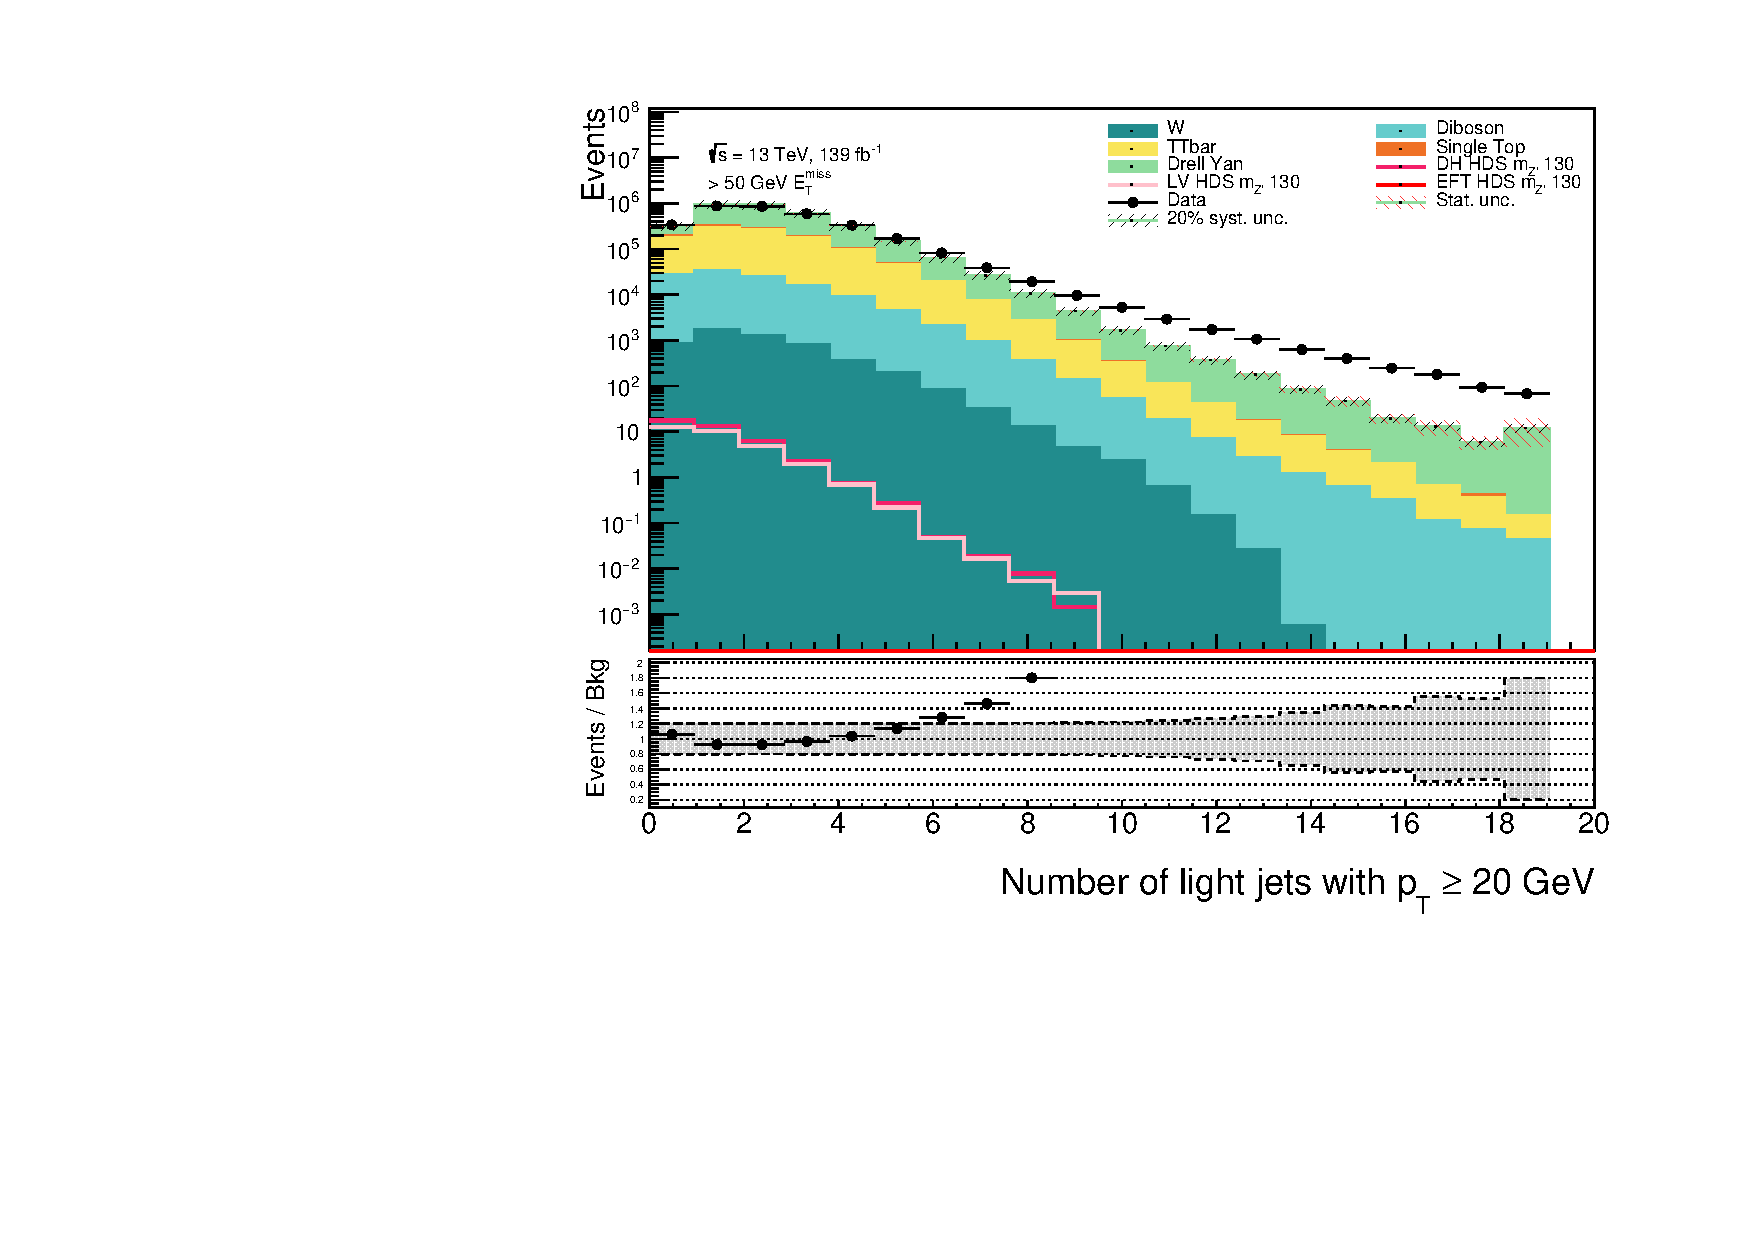
\includegraphics[width=\textwidth]{ljetsPt20.pdf}
%     \end{subfigure}
%     \hfill\begin{subfigure}[b]{0.49\textwidth}
%         \centering
%         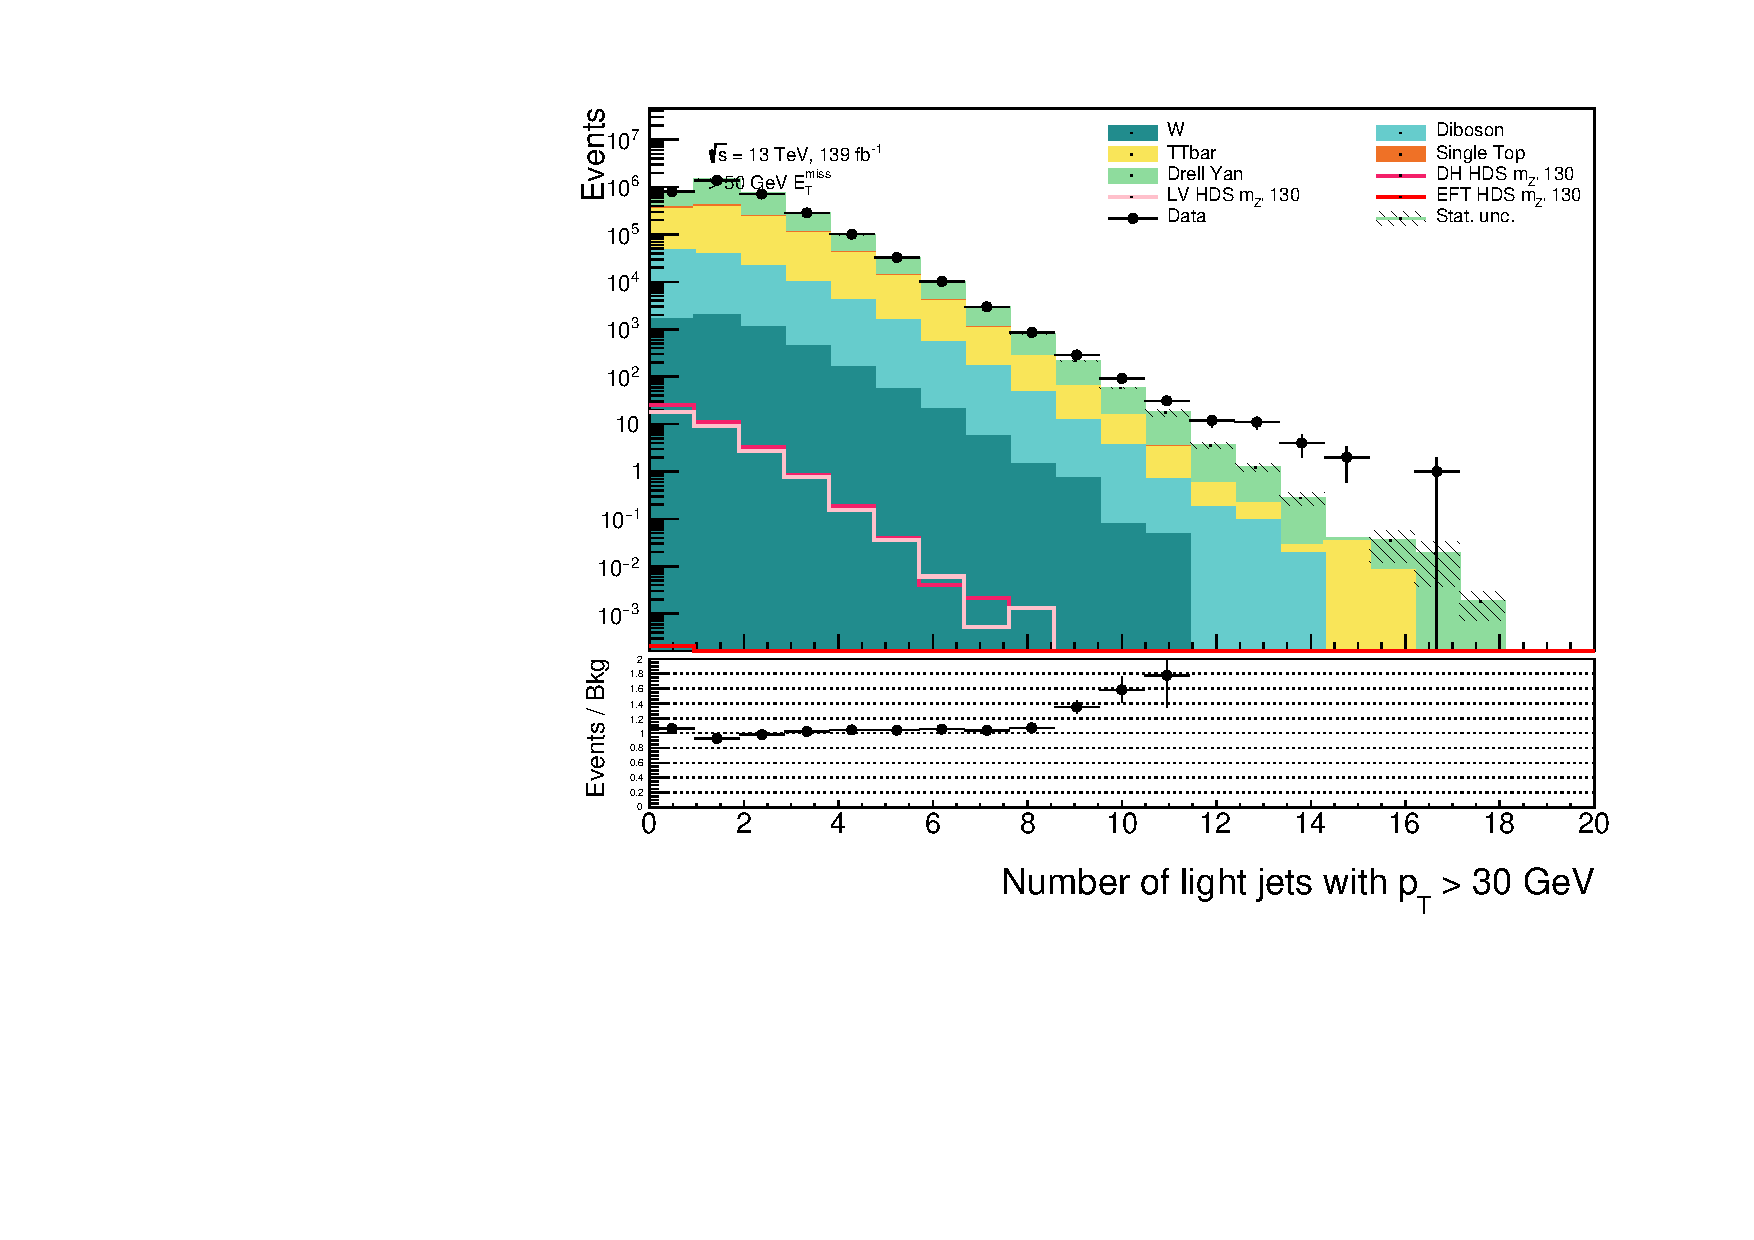
\includegraphics[width=\textwidth]{ljetsPt30.pdf}
%     \end{subfigure}
%     \hfill\begin{subfigure}[b]{0.49\textwidth}
%         \centering
%         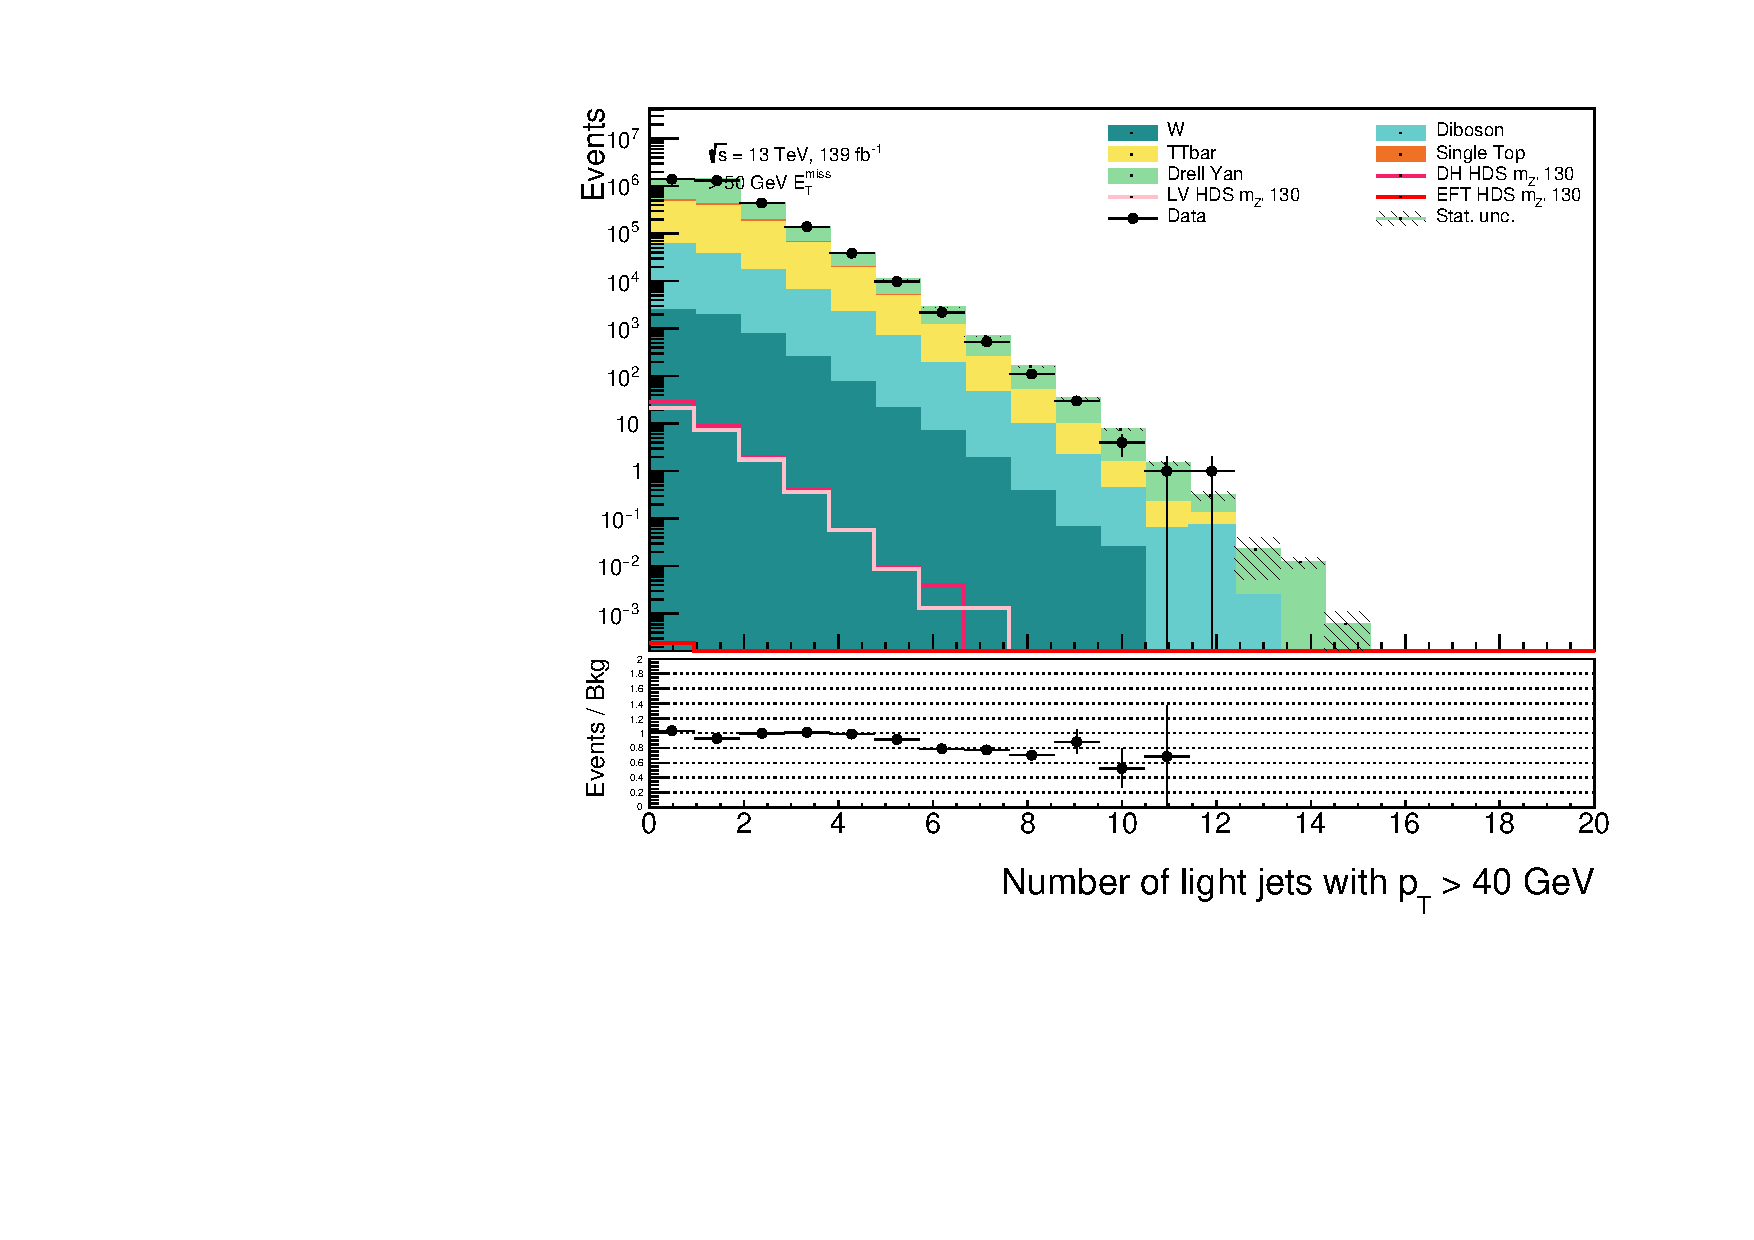
\includegraphics[width=\textwidth]{ljetsPt40.pdf}
%     \end{subfigure}
%     \hfill\begin{subfigure}[b]{0.49\textwidth}
%         \centering
%         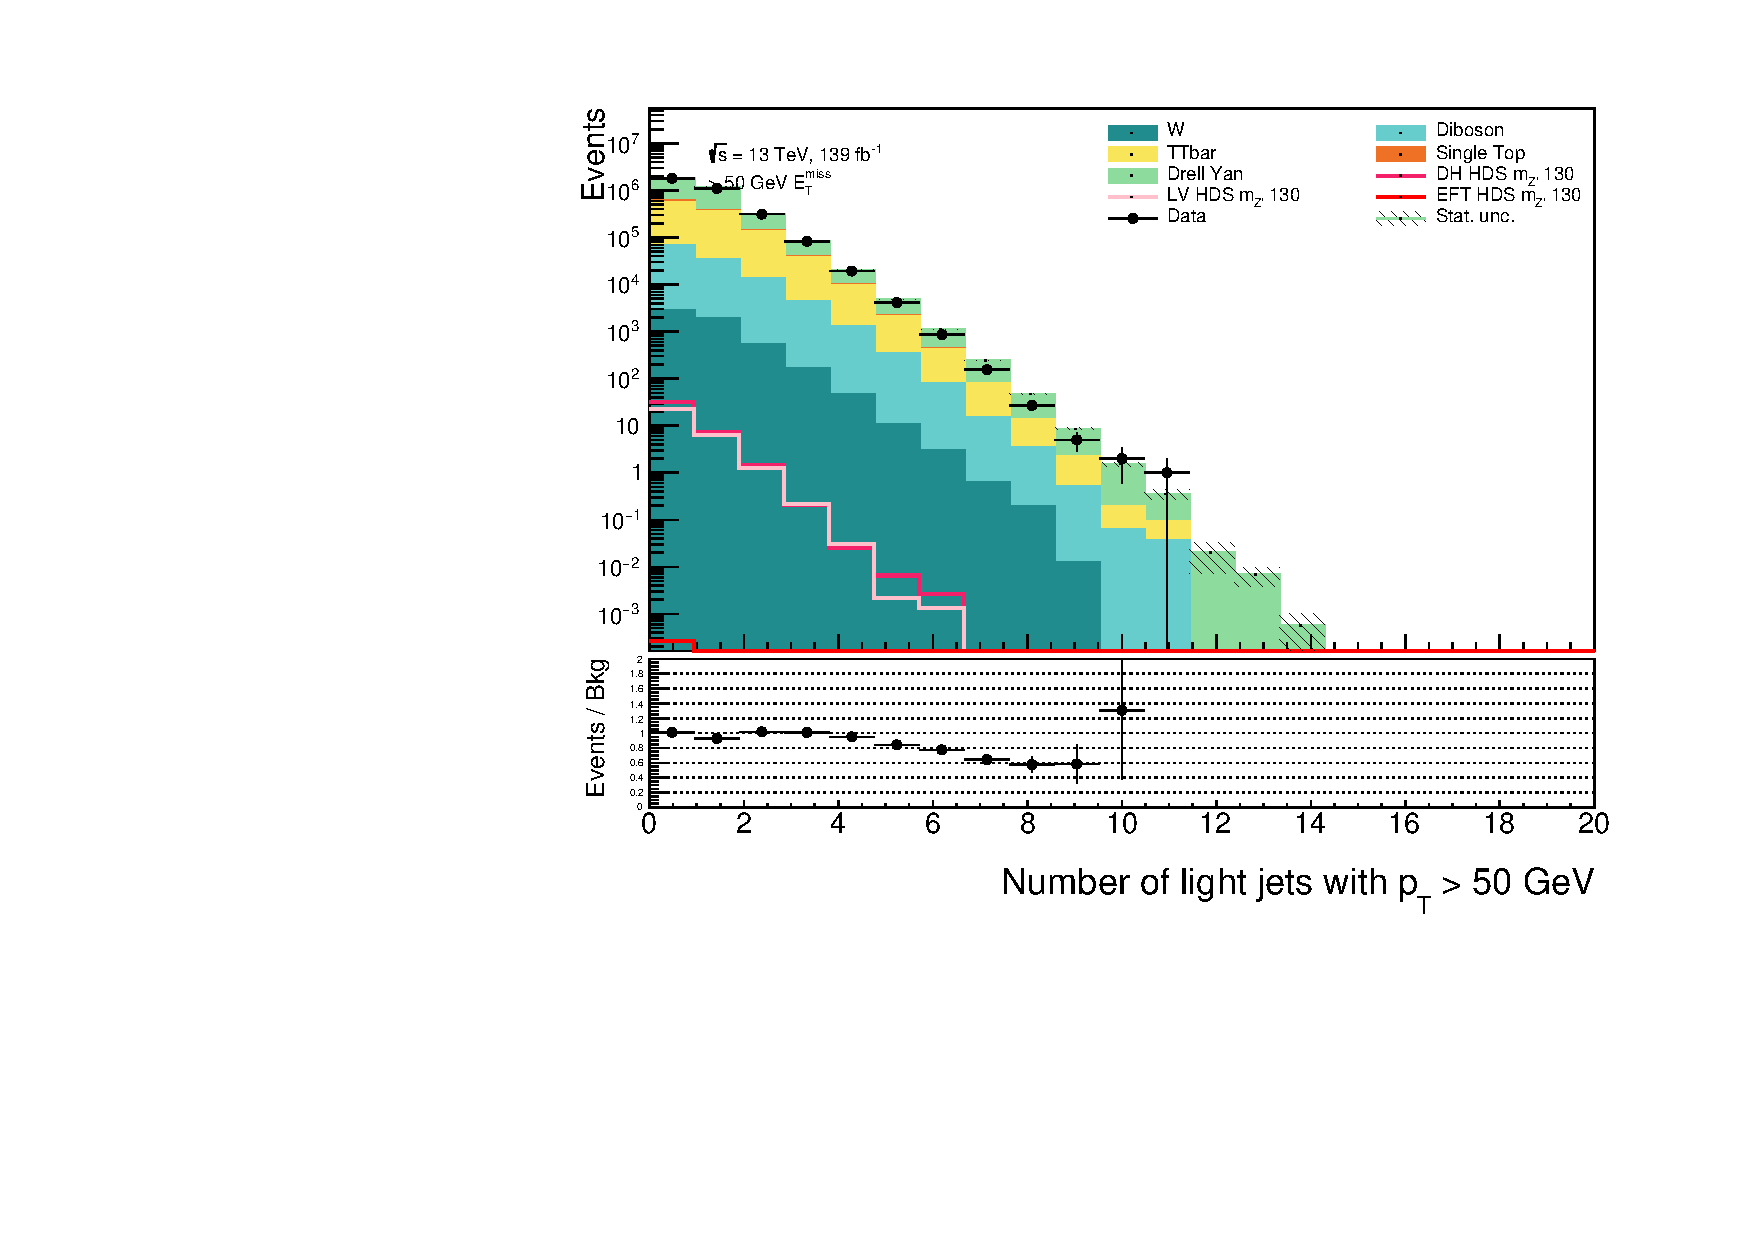
\includegraphics[width=\textwidth]{ljetsPt50.pdf}
%     \end{subfigure}
%     \hfill\begin{subfigure}[b]{0.49\textwidth}
%         \centering
%         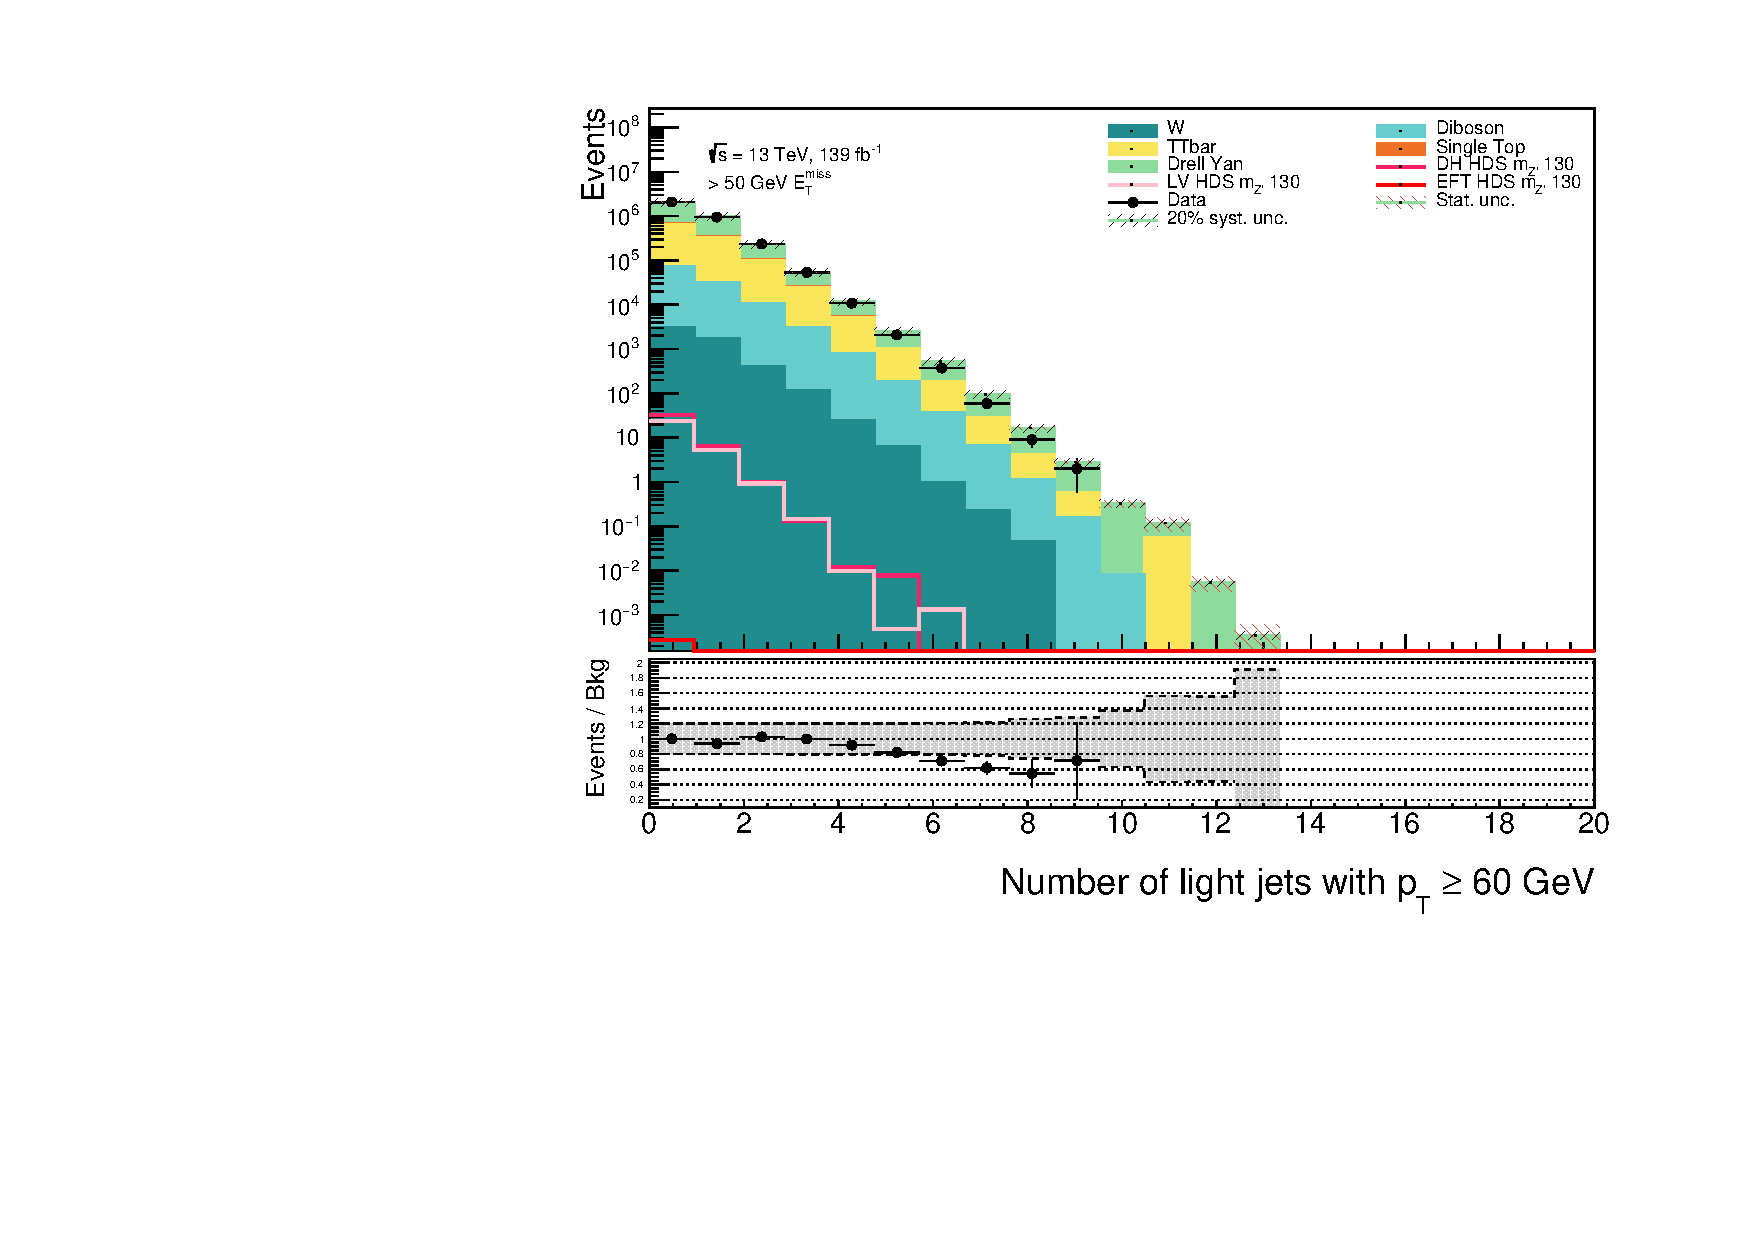
\includegraphics[width=\textwidth]{ljetsPt60.pdf}
%     \end{subfigure}
%     \caption{Data and MC agreement on number of light jets with different $p_T$ cuts in SR3.}
% \end{figure}

\clearpage


\end{document}